\RequirePackage{fix-cm}
\documentclass[oneside, a4paper]{book}
\usepackage[a4paper,width=150mm,top=25mm,bottom=25mm,bindingoffset=6mm]{geometry}


% Required for inserting images
\usepackage{eso-pic,graphicx}

% misc
\usepackage{caption}
\DeclareCaptionType{equ}[][]
%\captionsetup[equ]{labelformat=empty}

\usepackage{subcaption}
\usepackage{multicol}
\usepackage{float}
\usepackage{adjustbox} % oversized table

% Default font to sans serif
\renewcommand{\familydefault}{\sfdefault}
\RequirePackage[T1]{fontenc} 
\RequirePackage[tt=false, type1=true]{libertine} 
\RequirePackage[varqu]{zi4} 
% \RequirePackage[libertine]{newtxmath}

% chapters and headers
\usepackage[Conny]{fncychap}

\usepackage{fancyhdr}
\pagestyle{fancy}
\renewcommand{\headrulewidth}{0.1pt}
\renewcommand{\chaptermark}[1]{\markboth{\MakeUppercase{\textsf{#1}}}{}}
\renewcommand{\sectionmark}[1]{ \markright{\MakeUppercase{\textsf{\thesection\ #1}}}{} }

% algorithms
\usepackage{algorithm}
\usepackage{algpseudocode}

% FAT FONTS
\usepackage{bm} % bold fonts in math mode
\newcommand\fat[1]{{\boldmath{\textbf{#1}}}}
\newcommand\emphasis[1]{{\scshape\bfseries#1}}

% mathematical fonts and graphics
\usepackage{mathtools}
\usepackage{xfrac} % sfrac for diagonal slashes in fractions
\usepackage{amsfonts} % math fonts
\usepackage{dsfont} % math fonts
\usepackage{bbm} % mathbb fonts
\usepackage{mathrsfs} % fancy swirly font
\usepackage{gensymb} % degree sign

% draw graphs
\usepackage[inline]{asymptote}
\usepackage{qtree}
\usepackage{tikz}

% nicer fractions
\usepackage{xfrac}

% units
\usepackage{siunitx}

% plots
\usepackage{pgfplots}
\usepackage{pgfplotstable}
\usepgfplotslibrary{external}
\usepgfplotslibrary{patchplots}
\usepgfplotslibrary{groupplots}
\pgfplotsset{compat=1.18} 
\tikzexternalize[prefix=tikz,optimize=false]


% define the Spectral_r color scheme
\usepackage{xcolor}
\definecolor{Spectral0}{RGB}{158, 1, 66}
\definecolor{Spectral1}{RGB}{213, 62, 79}
\definecolor{Spectral2}{RGB}{244, 109, 67}
\definecolor{Spectral3}{RGB}{253, 174, 97}
\definecolor{Spectral4}{RGB}{254,224,139}

\definecolor{Spectral5}{RGB}{255,255,191}
\definecolor{Spectral6}{RGB}{230,245,152}
\definecolor{Spectral7}{RGB}{171,221,164}
\definecolor{Spectral8}{RGB}{102,204,204}
\definecolor{Spectral9}{RGB}{50,136,189}
\definecolor{Spectral10}{RGB}{94,79,162}
\pgfplotsset{
  colormap={Spectral_r}{
    rgb255(0cm)=(94,79,162)         % 0.0
    rgb255(1cm)=(50,136,189)        % 0.1
    rgb255(2cm)=(102,204,204)       % 0.2
    rgb255(3cm)=(171,221,164)       % 0.3
    rgb255(4cm)=(230,245,152)       % 0.4
    rgb255(5cm)=(255,255,191)       % 0.5
    rgb255(6cm)=(254,224,139)       % 0.6
    rgb255(7cm)=(253,174,97)        % 0.7
    rgb255(8cm)=(244,109,67)        % 0.8
    rgb255(9cm)=(213,62,79)         % 0.9
    rgb255(10cm)=(158,1,66)         % 1.0
    }
}


% get width of given text
\usepackage{calc}

% define a horizontal spacer
\newcommand\horizontalspacer[0]{\vspace{5pt}\noindent\textcolor{lightgray}{\rule{\textwidth}{1mm}}
\vspace{5pt}}

% clickable links
\usepackage{hyperref}
\hypersetup{
    colorlinks,
    citecolor=black,
    filecolor=black,
    linkcolor=black,
    urlcolor=black
}
% citations
\usepackage[
  backend=biber,
  sorting=none,
  style=phys,
]{biblatex}
\addbibresource{refs.bib}

% fancy boxes
\usepackage{fancybox}

% labels to enum items
\usepackage{enumitem}

% make empty lines skip
% \usepackage{parskip}

% ~~~~~~~~~ TYPESETTING AND OTHER MACROS ~~~~~~~~~~~~~~~~~~~~~

\newenvironment{absolutelynopagebreak}
  {\par\nobreak\vfil\penalty0\vfilneg
   \vtop\bgroup}
  {\par\xdef\tpd{\the\prevdepth}\egroup
   \prevdepth=\tpd}

% ~~~~~~~~~ AFANCY CHAPTER HEADINGS ~~~~~~~~~~~~~~~~~~~~~~~~~~~
\makeatletter
\def\thickhrulefill{\leavevmode \leaders \hrule height 1ex \hfill \kern \z@}
\def\@makechapterhead#1{%
  %\vspace*{50\p@}%
  \vspace*{10\p@}%
  {\parindent \z@ \centering \reset@font
        \thickhrulefill\quad
        \scshape \@chapapp{} \thechapter
        \quad \thickhrulefill
        \par\nobreak
        \vspace*{10\p@}%
        \interlinepenalty\@M
        \hrule
        \vspace*{10\p@}%
        \Huge {\textbf{#1}} \par\nobreak
        \par
        \vspace*{10\p@}%
        \hrule
    \vskip 40\p@
    % \vskip 100\p@
  }}
\def\@makeschapterhead#1{%
  %\vspace*{50\p@}%
  \vspace*{10\p@}%
  {\parindent \z@ \centering \reset@font
        \thickhrulefill
        \par\nobreak
        \vspace*{10\p@}%
        \interlinepenalty\@M
        \hrule
        \vspace*{10\p@}%
        \Huge \bfseries #1\par\nobreak
        \par
        \vspace*{10\p@}%
        \hrule
    \vskip 40\p@
    % \vskip 100\p@
  }}

  
\usepackage[pdftex,outline]{contour}

% ~~~~~~~~~ ALGORITHM MACROS ~~~~~~~~~~~~~~~~~~~~~~~~~~~~~~~~~
\newcommand{\var}[1]{\text{\texttt{#1}}}
\newcommand{\func}[1]{\text{\textsl{#1}}}

\makeatletter
\newcounter{phase}[algorithm]
\newlength{\phaserulewidth}
\newcommand{\setphaserulewidth}{\setlength{\phaserulewidth}}
\newcommand{\Phase}[1]{%
  \vspace{-1.25ex}
  % Top phase rule
  \Statex\leavevmode\llap{\rule{\dimexpr\labelwidth+\labelsep}{\phaserulewidth}}\rule{\linewidth}{\phaserulewidth}
  \Statex\strut\refstepcounter{phase}\textit{Step ~\thephase~--~#1}% Phase text
  % Bottom phase rule
  % \vspace{-1.25ex}\Statex\leavevmode\llap{\rule{\dimexpr\labelwidth+\labelsep}{\phaserulewidth}}\rule{\linewidth}{\phaserulewidth}
  }

\makeatother
\makeatother

\setphaserulewidth{.1pt}

% ~~~~~~~~~ MATH MACROS ~~~~~~~~~~~~~~~~~~~~~~~~~~~~~~~~~~~~~~

% abs value macro
% \DeclarePairedDelimiter\abs{\lvert}{\rvert}
\newcommand\abs[1]{\left|#1\right|}

\newcommand\dist[1]{\left|\left|#1\right|\right|}
\newcommand\arr[1]{\left\langle#1\right\rangle}

% define the laplace operator 
\newcommand*\Laplace{\mathop{}\!\mathbin\nabla^2}
\newcommand\vek[1]{\vec{\bm{#1}}}
\newcommand\mat[1]{{\mathds{#1}}}
\newcommand\br[1]{\left(#1\right)}

\DeclareMathOperator{\sgn}{sgn}
\DeclareMathOperator{\erf}{erf}

\DeclareMathOperator*{\argmax}{\arg\!\max}
\DeclareMathOperator*{\argmin}{\arg\!\min}

% ~~~~~~~~~ START ~~~~~~~~~~~~~~~~~~~~~~~~~~~~~~~~~~~~~~~~~~~

\captionsetup[figure]{font=footnotesize,labelfont=footnotesize,justification=centering}
\begin{document}
\begin{titlepage}
  \pagestyle{empty}

  % \AddToShipoutPictureBG*{
\includegraphics[width=\paperwidth,height=\paperheight]{images/title/titlesim.jpg}}

  \begin{center}
    \Huge\textbf{Equation of State Solvers for Smoothed Particle Hydrodynamics}\\
    \vspace{0.5cm}
    \Large{Julian Karrer}\\
    \vfill
    \begin{figure*}[h!]
      \centering
      \resizebox{10cm}{!}{$\frac{D\vek{v}}{Dt} = -\frac{1}{\rho} \nabla p + \nu \Laplace \vek{v} +\vek{b}^{ext}$}
      \caption*{The Navier-Stokes momentum equation for incompressible flow. This tile page itself is used as a simulation domain in which this equation is solved, highlighting the solver's ability to handle complex boundary conditions and resolve details while maintaining low levels of compression (here: $\rho^{max}_{err}<0.1\%$ for $N>250k$ particles).}
      % \caption{Colour coded velocity field of a simulation with 250000 particles, where the solver handles
      %   complex boundary conditions, turbulent flow at low viscosity and a pronounced free surface with less than
      %   0.1\% compression. \cite{ray-optics-book}}
      \label{fig:title-image}
    \end{figure*}
    \vfill
    \Large
    % \contour{black}{\textcolor{white}{Lab Course}}\\
    % \contour{black}{\textcolor{white}{Master of Science in Computer Science}}\\

    \vspace{5.2cm}
    % \vspace{0.5cm}
    % \large
    % Faculty of Engineering\\
    % Department of Computer Science\\
    % Supervised by Prof. Dr.-Ing. Matthias Teschner\\
    % \vspace{0.5cm}
    % % \includegraphics*[width=5cm]{images/title/ufr-?logo.png}
  \end{center}
\end{titlepage}
% \captionsetup[figure]{font=normalsize,labelfont=normalsize}

\tableofcontents
\newpage



\chapter{Introduction}

\chapter{Governing Equations of Fluid Flow}\label{chp:governing-equations}
In an attempt to create a numerical solver for fluid dynamics problems, the governing equations of the underlying physical process must first be understood and formulated. Only then can an appropriate discretization be applied to numerically solve for desired properties of a system. In this chapter, the abstractions of continuum mechanics are used as a framework to describe incompressible flow. Physical principles such as conservation of mass and momentum are used to derive the continuity and momentum equations which encode them, then augmented by constitutive relations which describe properties of Newtonian fluids to finally yield the Navier-Stokes equations as governing equations.
\autocite*{anderson}\autocite*{tutorial}

The particular form of these equations will favour a Lagrangian view of the system, in which the frame of reference in which quantities are described is advected along with the flow of the fluid itself, which will seamlessly integrate with the discretization scheme later used to derive workable numerical algorithms.



\section{Lagrangian and Eulerian Continuum Mechanics}
The purpose of our mathematical modelling of fluids is to simulate fluid dynamics at macroscopic scales with numerical methods. We know that fluids consist of innumerable molecules, and smaller particles yet, interacting in complex ways, which give rise to emergent properties that we observe on a macroscopic scale. Instead of resolving all scales and simulating from quantum mechanical principles up, we content with modelling the emergent properties themselves, focusing on the question of how fluids behave on our desired scales instead of what gives rise to such effects. Our macroscopic scale is so many orders of magnitude larger than the quantized world of particles, that we can reasonably assume quantities describing the fluid to be continuous and tackle them with the tools of calculus. This gives rise to the field of \emphasis{Continuum Mechanics}.\\
In the following derivations, two major points of view can be taken, which produce different but equivalent forms of equations: the Eulerian or conservation forms, and the Lagrangian or nonconservation forms of the equations\autocite*{anderson}.

Using the assumption from continuum mechanics that quantities of our fluid are continuously distributed in space and asserting that they be differentiable, we can define derivatives on them. The two major forms of equations arise from a different interpretation of the so-called substantial derivative\autocite*{anderson} or material derivative\autocite*{tutorial} $\frac{D}{Dt}$. This operator describes the instantaneous time rate of change of a quantity of a continuum element as it moves through space \autocite*{anderson}. This movement through space however can be observed from different frames of reference:
\begin{itemize}
    \item a frame that is advected along with the flow of the fluid, in which the continuum element observed appears unmoving
    \item a frame that is unmoving in space and located at a fixed point, observing the flow of the fluid as continuum elements move through it
\end{itemize}

For both frames of reference, it can be derived that the material derivative in vector notation is \autocite*{anderson}:

\begin{align}
    \frac{D}{Dt} = \underbrace{\frac{\partial }{\partial t}}_{\text{local derivative}} + \underbrace{(\vek{v}\cdot \nabla)}_{\text{convective derivative}}
\end{align}
where $\vek{v}$ is the velocity of the element and $\nabla$ denotes the differential operator $\left(\frac{\partial}{\partial x_0}, \frac{\partial}{\partial x_1}, \dots,  \frac{\partial}{\partial x_n}\right)^T$ in $n$ dimensions \autocite*{anderson}. If an Eulerian view is chosen, there is an additional term for the convective derivate, which describes a rate of change of a quantity at a fixed point due to movement of the fluid. If a Lagrangian view is taken, the reference frame is advected with the velocity $\vek{v}$, precisely such that the convective derivative is zero and the material derivative simply becomes the total time derivative of a quantity. The difference between the two views is illustrated in \autoref{fig:lagrange-euler-1d}. In a way, the Lagrangian frame of reference is chosen precisely such that only local derivatives suffice to describe material derivatives by using a coordinate transformation defined by the velocity field.

How this simpler, Lagrangian form can be used largely depends on the later choice of discretization: discretizing space and tracking the fluid that moves through it favours an Eulerian framework, while discretizing the continuum into particles and sampling quantities only at advected particle positions makes the Lagrangian view convenient.\\
As is common for SPH discretizations, we will elect the Lagrangian view since it not only harmonizes well with particle-based discretizations but holds additional desirable properties such as making conservation of mass trivial to implement and enabling solving the Navier-Stokes equations for primitive quantities instead of flux quantities that may cause drift instead of oscillations due to numerical inaccuracy. We state all following equations in the Lagrangian, nonconservation form.

\begin{figure}
    \begin{center}
        \begin{subfigure}[t]{0.5\textwidth}
            \centering
            \begin{asy}
                import graph;
                defaultpen(fontsize(8pt));
                size(7cm,0);
                real xmin = -3;
                real xmax = 3;
                real ymin = 0;
                real ymax = 3;

                real b(real x) {return x < -0.7?0:(x>0.7?0:ymax);}
                real f(real x) {
                        real t = 0.3;
                        real sum = 0;
                        int n = 100;
                        real dx = 2.0 / n;
                        for (int i = 0; i <= n; ++i) {
                                real xi = -1 + i * dx;
                                sum += exp(-((x - xi) * (x - xi)) / (4 * t)) * b(xi);
                            }
                        return sum / (sqrt(4 * 3.141592653589793 * t)) * dx;
                    }

                draw((0, b(0)) .. (0, f(0)), black, arrow=Arrows(TeXHead));
                label("local",(0,(b(0)-f(0))/2.+ f(0)), E);

                draw(graph(new real(real x) { return b(x); },xmin,xmax, n=1000), heavyblue);
                draw(graph(new real(real x) { return f(x); },xmin,xmax, n=1000), lightblue+dashed);
                label("$A(\vek{x},t)$",(-0.69, b(-0.69)),NW, heavyblue);
                label("$A(\vek{x},t+\Delta t)$",(2.0, f(2.0)),NE, lightblue);

                // draw axis
                arrowbar axisarrow = Arrow(TeXHead);
                draw((xmin,0) -- (xmax,0), arrow=axisarrow);
                label("$x$",(xmax,0),S);
                draw((xmin+0.5,ymin) -- (xmin+0.5,ymax+0.5), arrow = axisarrow);
                label("$A$",(xmin+0.5,ymax+0.5),E);

                draw((0,ymin) -- (0,ymax+0.5),  black+dotted);
                dot("$\vek{x}_i$",(0,ymin),S);
            \end{asy}
            \caption{Lagrangian view}
        \end{subfigure}%
        ~
        \begin{subfigure}[t]{0.5\textwidth}
            \centering
            \begin{asy}
                import graph;
                defaultpen(fontsize(7.5pt));
                size(7cm,0);
                real xmin = -3;
                real xmax = 3;
                real ymin = 0;
                real ymax = 3;

                real b(real x) {return x < -0.7?0:(x>0.7?0:ymax);}
                real f(real x) {
                        real t = 0.3;
                        real sum = 0;
                        int n = 100;
                        real dx = 2.0 / n;
                        for (int i = 0; i <= n; ++i) {
                                real xi = -1 + i * dx;
                                sum += exp(-((x - xi) * (x - xi)) / (4 * t)) * b(xi);
                            }
                        return sum / (sqrt(4 * 3.141592653589793 * t)) * dx;
                    }

                draw((0, b(0)) .. (0, f(0)), black, arrow=Arrows(TeXHead));
                draw((-0.6, f(0)) .. (0.6, f(0)), black+dotted);
                label("local",(0,(b(0)-f(0))/2.+ f(0)), W);
                draw((0, f(0)) .. (0, f(-0.6)), black, arrow=Arrows(TeXHead));
                label("convective",(0,(f(0)-f(-0.6))/2.+ f(-0.6)), W);

                draw(graph(new real(real x) { return b(x+0.6); },xmin,xmax, n=1000), heavyblue);
                draw(graph(new real(real x) { return f(x-0.6); },xmin,xmax, n=1000), lightblue+dashed);
                label("$A(\vek{x},t)$",(-0.69-0.6, b(-0.69)),NW, heavyblue);
                label("$A(\vek{x},t+\Delta t)$",(2.0, f(2.0)+0.2),NE, lightblue);

                // draw axis
                arrowbar axisarrow = Arrow(TeXHead);
                draw((xmin,0) -- (xmax,0), arrow=axisarrow);
                label("$x$",(xmax,0),S);
                draw((xmin+0.5,ymin) -- (xmin+0.5,ymax+0.5), arrow = axisarrow);
                label("$A$",(xmin+0.5,ymax+0.5),E);

                draw((0,ymin) -- (0,ymax+0.5),  black+dotted);
                dot("$\vek{x}$",(0,ymin),S);
                dot("$\vek{x}_i(t)$",(-0.6,ymin),SW);
                dot("$\vek{x}_i(t+\Delta t)$",(0.6,ymin),SE);
            \end{asy}
            \caption{Eulerian view}
        \end{subfigure}
    \end{center}
    \caption{A field quantity $A$ in one dimension is shown at some time $t$ and a later time $t+\Delta t$ where the distribution of $A$ has changed due to some diffusive process and the quantity was advected in positive $x$-direction. In the Lagrangian view, changes in a quantity $A$ are evaluated at the advected position $\vek{x}_i$ at any point in time and only the local derivative is needed to describe the change in $A$ at $\vek{x}$. In the Eulerian view there are two reasons for $A$ at a point $\vek{x}$ fixed in space to change: the local derivative due to the diffusive process and the convective derivative due to the advection of the quantity with the velocity field.}
    \label{fig:lagrange-euler-1d}
\end{figure}

\section{The Continuity Equation}\label{sec:continuity-equation}
Using the Lagrangian view of continuum mechanics, we can apply laws of conservation to derive equations that express invariants of each fluid element with respect to time, which is an important step towards describing the dynamics of the system as time evolves. One such equation is the \emphasis{continuity equation}, which expresses conservation of mass:\\
Consider an infinitesimally small volume element $\delta \mathcal{V}$ with density $\rho$. The mass of the volume $\delta m$ is simply\autocite*{anderson}:
\begin{equation}\delta m = \rho \delta\mathcal{V}\label{eq:infintitesimal_volume}\end{equation}
and is invariant under the material derivative in the Lagrangian reference frame \autocite*{anderson}:
\begin{align}
    \frac{D\delta m}{D t} & = 0                                                                                                 & \textit{conservation of mass}                    \\
                          & = \frac{D \rho \delta\mathcal{V}}{Dt}                                                               & \textit{identity \ref{eq:infintitesimal_volume}} \\
                          & = \delta\mathcal{V} \frac{D \rho}{Dt} + \rho \frac{D \delta\mathcal{V}}{Dt}                         & \textit{product rule of calculus}                \\\label{eq:cont-eq-unfinished}
                          & =  \frac{D \rho}{Dt} + \rho \left(\frac{1}{\delta\mathcal{V}} \frac{D \delta\mathcal{V}}{Dt}\right) & \textit{divide by $\delta \mathcal{V}$}
\end{align}

We can now apply the \emphasis{divergence theorem} to relate $\frac{D\mathcal{V}}{D t}$ to the divergence of the velocity across the volume of the element, where $\partial \mathcal{V}$ is its surface and $\vek{n}$ the corresponding unit normal vector \autocite*{anderson}:

\begin{equation}\label{eq:div-theorem}
    \frac{D\mathcal{V}}{D t} =
    \oint_{\partial \mathcal{V}} \vek{v} \cdot \vek{n}\, dS =
    \int_{\mathcal{V}} \left( \nabla\cdot \vek{v}\right)\,d\mathcal{V}
\end{equation}

As the volume $\mathcal{V}$ approaches the infinitesimal volume element $\delta \mathcal{V}$ of interest, the velocity in the volume becomes constant, the integral vanishes, and it holds that \autocite*{anderson}:


\begin{equation}\label{eq:div-theorem-on-dV}
    \frac{D(\delta \mathcal{V})}{D t} = \left( \nabla\cdot \vec{v}\right) \delta \mathcal{V}
\end{equation}

Substituting \autoref{eq:div-theorem-on-dV} into \autoref{eq:cont-eq-unfinished} we finally obtain the continuity equation:

\begin{equation}\label{eq:continuity-eq}
    \text{\fbox{$\frac{D\rho}{D t} + \rho\left( \nabla \cdot \vek{v} \right) = 0$}}
\end{equation}

This is one of the Navier-Stokes equations in its derivative form, as opposed to the more general integral form \autocite*{anderson}. When we additionally assume that the fluid is incompressible across a wide range of pressures, as is often done when simulating hydrodynamics, we can assert that the density of the fluid element in a Lagrangian reference frame is constant, meaning:
\begin{equation}\label{eq:continuity-means-density-dt-zero}
    \frac{D\rho}{D t} = 0
\end{equation}
and therefore the velocity field of the flow for constant density is divergence-free\autocite*{continuum-intro}:
\begin{equation}\label{eq:continuity-means-velocity-divergence-zero}
    \nabla\cdot \vek{v} = 0
\end{equation}
In the following sections, the fluid will generally be assumed to be incompressible.\\

An alternative derivation of the continuity equation uses the \emphasis{Reynolds Transport Theorem}, which describes the material derivative of a scalar or tensor quantity $q(\vek{x}, t)$ integrated over a volume as the sum of its time rate of change within the volume and the flux of the quantity through the volume's surface \autocite*{continuum-intro}:
\begin{equation}\label{eq:reynolds-transport-theorem}
    \frac{D}{D t}\int_\mathcal{V} q(\vek{x}, t)\,dV = \int_\mathcal{V} \frac{\partial q(\vek{x}, t)}{\partial t} \,dV + \oint_{\partial\mathcal{V}}  q(\vek{x}, t)(\vek{v} \cdot \vek{n})\,dS
\end{equation}

This derivation goes as follows \autocite*{continuum-intro}:

\begin{align}
    0 & = \frac{D}{Dt} \int_\mathcal{V}\rho\,dV                                                                                & \textit{conservation of mass}                   \\
      & = \int_\mathcal{V} \frac{\partial\rho}{\partial t} \,dV + \oint_{\partial \mathcal{V}} \rho (\vek{v}\cdot\vek{n}) \,dS & \textit{Reynolds Transport Theorem}             \\
      & = \int_\mathcal{V} \frac{\partial\rho}{\partial t} \,dV + \int_{\mathcal{V}} \nabla \cdot (\rho \vek{v}) \,dV          & \textit{Divergence Theorem}                     \\
      & = \int_\mathcal{V} \left(\frac{\partial\rho}{\partial t} + \nabla \cdot (\rho \vek{v})\right) \,dV                     & \textit{combine integrals}                      \\
      & = \int_\mathcal{V} \left(\frac{D\rho}{D t} + \rho \nabla \cdot  \vek{v}\right) \,dV                                    & \textit{constant density, Lagrangian framework} \\
      & \overset{\forall\mathcal{V}}{\Longrightarrow} \frac{D\rho}{D t} + \rho \left(\nabla \cdot  \vek{v}\right) = 0          & \textit{integral holds for all $\mathcal{V}$}
\end{align}

This use of the Reynolds Transport Theorem is very similar to the derivation that follows in \autoref{sec:momentum-equation}, which is why this alternative derivation was stated.

\section{The Cauchy Momentum Equation}\label{sec:momentum-equation}

Mass is not the only conserved quantity that can be formulated in terms of a volume integral which can be transformed into a more convenient form using Reynolds Transport Theorem: a vital step in the derivation of the Navier-Stokes equations comes from applying the same concept to the conservation of momentum. In fact, the \emphasis{Cauchy momentum equation}, which is the general case of the more specific momentum equation used in the Navier-Stokes equations, can be derived similarly to \autoref{sec:continuity-equation}, additionally using the continuity equation itself and Newton's second law.

We begin by observing that the change of momentum of a fluid volume $\mathcal{V}$ can be defined as the material derivative of the momentum $\int_\mathcal{V}(\rho\vek{v})\,dV$ and simplify the resultant expression\autocite*{continuum-intro}:
\begin{align}
     & \frac{D}{Dt}\int_\mathcal{V}(\rho\vek{v})\,dV                                                                                                                    & \textit{define change in momentum}      \\ & = \int_\mathcal{V} \frac{\partial (\rho\vek{v})}{\partial t}\,dV + \oint_{\partial \mathcal{V}} \rho \vek{v} (\vek{v} \cdot \vek{n})\,dS & \textit{Reynolds Transport Theorem \ref{eq:reynolds-transport-theorem}} \\
     & = \int_\mathcal{V}\frac{D}{Dt}(\rho\vek{v})\,dV + \int_\mathcal{V} (\rho\vek{v} )\nabla\cdot\vek{v} \,dV                                                         & \textit{Divergence Theorem}             \\
     & = \int_\mathcal{V} \rho\frac{D\vek{v}}{Dt} + \vek{v}\frac{D\rho}{Dt} + (\rho\vek{v}) \nabla\cdot\vek{v} \,dV                                                     & \textit{product rule on first integral} \\
     & = \int_\mathcal{V} \rho\frac{D\vek{v}}{Dt} + \vek{v} \underbrace{\left( \frac{D\rho}{Dt} + \rho \nabla\cdot\vek{v} \right)}_{\text{continuity equation} =0} \,dV & \textit{factor out $\vek{v}$}           \\\label{eq:momentum-lhs}
     & = \int_\mathcal{V} \rho\frac{D\vek{v}}{Dt} \,dV
\end{align}

Then, we use Newton's second law, best known in its form $F=m\vek{a}$, to assert that this change in momentum $m\vek{a}$ is equal to the sum of forces exerted on the fluid volume, which can be decomposed into body forces $\vek{b}^{ext}$ per unit mass\autocite*{continuum-intro} that act on the entire fluid mass homogeneously 'at a distance'\autocite*{anderson}, like gravity for example, and into surface forces described by stress vectors $\vek{t}$ integrated over the fluid element's surface\autocite*{continuum-intro}:
\begin{equation}
    \int_\mathcal{V} \rho\frac{D\vek{v}}{Dt} \,dV = \oint_\mathcal{\partial V}\vek{t}\,dS + \rho\vek{b}^{ext}
\end{equation}
One can define the \emphasis{Cauchy stress tensor} $\mat{T}$ (sometimes referred to as $\mat{\sigma}$) for the material such that it satisfies\autocite*{continuum-intro} $\mat{T}\vek{n} = \vek{t}$. Then, the divergence theorem may be applied again and the total forces acting on the fluid element can be written as:
\begin{equation}\label{eq:momentum-total-forces}
    \int_\mathcal{V}\nabla\cdot\mat{T}\,dV + \rho\vek{b}^{ext}
\end{equation}

Setting the expressions for total force in \autoref{eq:momentum-total-forces} and total change of momentum in \autoref{eq:momentum-lhs} equal according to Newton's Law, we obtain:
\begin{align}
    \int_\mathcal{V}  \rho\frac{D\vek{v}}{Dt} - \nabla\cdot\mat{T} - \rho\vek{b}^{ext} \,dV = 0
\end{align}
From this, we have obtained the \emphasis{Cauchy Momentum Equation} as our equation of motion\autocite*{tutorial}:

\begin{equation}\label{eq:cauchy-momentum-eq}
    \text{\fbox{$\rho\frac{D\vek{v}}{Dt} =  \nabla\cdot\mat{T} + \rho\vek{b}^{ext}$}}
\end{equation}

\section{The Lagrangian Navier-Stokes Equations}
With the Cauchy momentum equation we have reached the end of what can be modelled using general physical principles and continuum mechanics and is valid for a range of materials. To close the system of equations for fluid flow, generality must be given up and specific assumptions about the behaviour of fluids must be used to model the specific stress tensor $\mat{T}$ representing incompressible, linearly viscous or Newtonian fluids. In order to derive the form of the tensor, we make the further assumptions about the fluid that will later be clarified:
\begin{enumerate}
    \item Fluids cannot sustain shear stresses when in rigid body motion.\label{enum:ns-fluid-cant-sustain-shear}
    \item Viscosity depends on the symmetric component of the gradient of velocity, it is linearly proportional to the rate of deformation tensor.\label{enum:ns-vis-prop-rate-of-deform}
\end{enumerate}


All remaining terms of the Cauchy momentum equation are clear, only the stress tensor $\mat{T}$ needs to be elaborated upon. First, it can be noted that $\mat{T}$ is a linear transformation\autocite*{continuum-intro} and that the tensor is symmetric\autocite*{continuum-intro}, as in equal to its transpose $\mat{T}^T = \mat{T}$ or $\mat{T}_{ij} = \mat{T}_{ji}$. This means that in three dimensions for example, only six degrees of freedom actually exist in this tensor\autocite*{incompressible-flow-volker}.

The element $\mat{T}_{ij}$ expresses a stress along some axis $\vek{e_i}$ acting on a plane perpendicular to $\vek{e_j}$, which means that the diagonal elements $\mat{T}_{ii}$ are normal stresses called \textit{tensile stresses} for negative values and \textit{compressive stresses} for positive values of $\mat{T}_{ii}$\autocite*{continuum-intro}, while $\forall i\neq j:\,\mat{T}_{ij}$ refer to \textit{shear stresses}\autocite*{anderson}.\\


To make this tensor more tractable, it can be assumed that a fluid is a material which cannot sustain shear stresses when in rigid body motion, including rest\autocite*{continuum-intro} (assumption \ref{enum:ns-fluid-cant-sustain-shear}) - this means that when in rigid body motion, the stress vector on any plane is normal to that plane\autocite*{continuum-intro}, the stress is therefore isotropic and $\mat{T}$ must be represented by the only isotropic second order tensor $\lambda\mat{\mat{1}}$ or $\lambda\delta_{ij}$ for some $\lambda\in\mathds{R}$ where $\delta_{ij}$ is the Kronecker delta\autocite*{course-notes-12800}. This motivates a decomposition of $\mat{T}$ for any general motion into a sum of an isotropic tensor describing \textit{volumetric stress} caused by pressure forces and the \textit{deviatoric stress} $\mat{V}$ which simply describes deviation of the total stress $\mat{T}$ from the volumetric stress\autocite*{derivation-ns-undergrad}:
\begin{align}\label{eq:stress-tensor-decomp}
    \mat{T} = \mat{V} -p\mat{1}
\end{align}
Conventionally, the pressure $p$ is defined such that a positive pressure causes a negative stress, meaning the pressure acts normal to the surface and is directed into the fluid volume $\mathcal{V}$\autocite*{incompressible-flow-volker}. For a fluid at rest $\mat{V}_{ij} = 0$ holds and the normal stress is isotropically $-p$ according to \textit{Pascal's law}\autocite*{course-notes-12800}. \autoref{eq:stress-tensor-decomp} decomposes stresses into a part caused by pressure and one caused by viscosity, which is why $\mat{V}$ is sometimes referred to as the \textit{viscous stress tensor}\autocite*{incompressible-flow-volker}. Viscosity can be thought of as internal friction in a fluid or its resistance to deformation. \\

The remaining term $\mat{V}$ is caused by viscosity and modelled according to assumption \ref{enum:ns-vis-prop-rate-of-deform} in terms of the gradient of the velocity. This makes intuitive sense: where the velocity is homogeneous, and the gradient is zero, there is no friction between fluid elements - where the velocity differs greatly, there is more friction. Since velocity is a vector quantity, the gradient $\nabla\vek{v}$ is a tensor\autocite*{incompressible-flow-volker}:
\begin{equation}
    (\nabla \vek{v})_{ij} = \partial_j v_i = \frac{\partial v_i}{\partial x_j}
\end{equation}
As always, we can decompose this tensor $\mat{L} := \nabla \vek{v} $ into a sum of a symmetric and an antisymmetric part \autocite*{continuum-intro}:
\begin{align}
    \mat{L} & = \mat{D} + \mat{W}                           \\
    \mat{D} & = \frac{1}{2}\left(\mat{L} + \mat{L}^T\right) \\
    \mat{W} & = \frac{1}{2}\left(\mat{L} - \mat{L}^T\right) \\
\end{align}

$\mat{D}$ is referred to as the \emphasis{rate of deformation tensor} and $\mat{W}$ is called the \emphasis{spin tensor}.\\


This decomposition is convenient since the spin tensor does not contribute to viscosity  and only the rate of deformation tensor may be focused on. Note that since the deviatoric stress $\mat{V}$ we are trying to approximate is symmetric, and it only makes sense to use the symmetric component of the velocity gradient to model it.

Intuitively, the spin tensor encodes the rotational component of the velocity gradient, and a steadily rotating fluid (where $\mat{D}_{ij}=0$) is like a rigid body rotation: the relative positions of the fluid elements do not change, only their orientation with respect to a fixed reference frame, and therefore there is no friction. There is a vector $\vek{\omega}$ such that for any $\vek{v}$ it holds that $\mat{W}\vek{v} = \vek{\omega} \times \vek{v}$, where $\vek{\omega}$ points in the axis of rotation with a length of the angular velocity \autocite*{continuum-intro}. This is why the spin tensor is closely related to the vorticity tensor $2\mat{W}$\autocite*{continuum-intro}. In fact, enforcing that viscosity shall not affect the rotational component of velocity gradients and preserving accurate vorticity is key to accurately simulating turbulences in incompressible flows and conserving angular momentum \autocite*{vorticity-micropolar}.

Focusing further on the rate of deformation tensor, assumption \ref{enum:ns-vis-prop-rate-of-deform} can now fully be appreciated. One defining characteristic of Newtonian fluids is the assumption dating back to Isaac Newton that viscosity depends \textit{linearly} on the rate of deformation tensor \autocite*{anderson}. This means that terms of an order higher than linear may be neglected for small velocity gradients\autocite*{incompressible-flow-volker} and constant terms cannot occur since shear stress is only proportional to the rate of deformation, not deformation itself\autocite*{continuum-intro}: if a shear stress is applied to a fluid it will eventually continuously deform at some non-zero rate but will remain in that deformed state if the stress is removed, unlike purely elastic materials\autocite*{continuum-intro}. In other words $\mat{V}$ must vanish when the velocity is homogeneous since there is no friction in that case \autocite*{incompressible-flow-volker}.

We now know that for incompressible fluids $\mat{V}$ is of the form \autocite*{incompressible-flow-volker}:
\begin{align}
    \mat{V} & = 2\mu \mat{D}+ \lambda (\nabla\cdot\vek{v})\mat{1}                                                                                                  \\
            & = \frac{2\mu}{2}\left((\nabla \vek{v}) + (\nabla \vek{v})^T\right) + \underbrace{\lambda (\nabla\cdot\vek{v})\mat{1}}_{\text{incompressibility = 0}} \\
            & = \mu\left((\nabla \vek{v}) + (\nabla \vek{v})^T\right)
\end{align}
where $\mu$ is the dynamic viscosity\autocite*{anderson} or first-order viscosity\autocite*{incompressible-flow-volker}. A second-order viscosity $\lambda$ exists for compressible flows\autocite*{anderson}, but can be neglected here.

Combining the deviatoric stress with the volumetric stress, the \emphasis{constitutive relation} for the stress tensor $\mat{T}$ of an incompressible, Newtonian fluid is finally obtained\autocite*{tutorial}:
\begin{equation}\label{eq:consistutive-relation}
    \text{\fbox{$\mat{T} = -p\mat{1} + \mu\left((\nabla \vek{v}) + (\nabla \vek{v})^T\right)$}}
\end{equation}

With the constitutive relation in hand, the Cauchy momentum equation can be revisited, and \autoref{eq:consistutive-relation} can be inserted into \autoref{eq:cauchy-momentum-eq}:
\begin{align}
    \label{eq:ns-deriv-step-1}\rho\frac{D\vek{v}}{Dt} & =  \nabla\cdot\left(-p\mat{1} + \mu\left((\nabla \vek{v}) + (\nabla \vek{v})^T\right)\right) + \rho\vek{b}^{ext}                                                         & \textit{insert Eq. \ref{eq:consistutive-relation} into Eq. \ref{eq:cauchy-momentum-eq}} \\
    \label{eq:ns-deriv-step-2}\rho\frac{D\vek{v}}{Dt} & = \nabla\cdot (-p\mat{1}) + \mu\nabla\cdot\left((\nabla \vek{v}) + (\nabla \vek{v})^T\right)+\rho\vek{b}^{ext}                                                           & \textit{$\nabla\cdot$ is linear}                                                        \\
    \label{eq:ns-deriv-step-3}\frac{D\vek{v}}{Dt}     & = -\frac{1}{\rho}\nabla p + \nu\nabla\cdot\left((\nabla \vek{v}) + (\nabla \vek{v})^T\right)+\vek{b}^{ext}                                                               & \textit{$\nabla\cdot (-p\mat{1}) = -\nabla p$, divide by $\rho$}                        \\
    \label{eq:ns-deriv-step-4}\frac{D\vek{v}}{Dt}     & = -\frac{1}{\rho}\nabla p + \nu\left(\underbrace{\nabla\cdot(\nabla \vek{v})}_{=\Laplace\vek{v}} + \underbrace{\nabla\cdot(\nabla \vek{v})^T}_{=0} \right)+\vek{b}^{ext} & \textit{$\nabla\cdot$ is linear}                                                        \\
    \label{eq:ns-deriv-step-5}\frac{D\vek{v}}{Dt}     & = -\frac{1}{\rho}\nabla p + \nu\Laplace\vek{v}+\vek{b}^{ext}                                                                                                             &
\end{align}

A few things of note happen in this derivation:
\begin{itemize}
    \item The kinematic viscosity $\nu$ is defined as $\frac{\mu}{\rho}$ and inserted in \autoref{eq:ns-deriv-step-3}
    \item The identity $\nabla\cdot(-p\mat{1}) = -\nabla\cdot\begin{bmatrix}
                  p & 0 & 0 \\
                  0 & p & 0 \\
                  0 & 0 & p \\
              \end{bmatrix} = -\begin{bmatrix}
                  \sfrac{\partial p}{\partial x} \\
                  \sfrac{\partial p}{\partial y} \\
                  \sfrac{\partial p}{\partial y} \\
              \end{bmatrix} = -\nabla p$ is used in \autoref{eq:ns-deriv-step-3}.
    \item For sufficiently smooth $\vek{v}$ and $\nabla\cdot\vek{v}=0$ one can show using the Theorem of Schwarz that $\nabla\cdot(\nabla \vek{v})=\Laplace\vek{v}$ as annotated in \autoref{eq:ns-deriv-step-4}\autocite*{incompressible-flow-volker}.
    \item Similarly, in \autoref{eq:ns-deriv-step-4} $\nabla\cdot(\nabla\vek{v}^T) = \nabla(\nabla\cdot\vek{v}) =0$ is used\autocite*{incompressible-flow-volker}, since the continuity equation for fluids of homogeneous density implies $\nabla\cdot\vek{v}=0$.
\end{itemize}

With all this, the final Navier-Stokes momentum equation for incompressible Newtonian fluids in Lagrangian form is obtained in step \ref{eq:ns-deriv-step-5}:

\begin{equation}\label{eq:navier-stokes-momentum}
    \text{\fbox{$\frac{D\vek{v}}{Dt}=-\frac{1}{\rho}\nabla p+\nu\Laplace\vek{v}+\vek{b}^{ext}$}}
\end{equation}

\section{Equations of State}

Although the momentum equation typically takes centre stage when discussing the Navier-Stokes equations, it is important to realize that the complete Navier-Stokes equations actually refer to a set of equations and the momentum equation cannot function on its own. At the very least, the continuity equation should be included, sometimes accompanied by an energy balance equation which is crucial to heat transport problems and formulates conservation of energy in viscous flows\autocite*{anderson}. For the dynamics of the systems considered here, the continuity and momentum equations appear to be sufficient, but one field quantity remains elusive until now: We have yet to discuss how to compute pressure.\\


When incompressibility is strongly enforced, the continuity equation is a constraint on the momentum equation that $p$ can be chosen to fulfil, making it a Lagrange multiplier to the equation\autocite*{tutorial}. Since strongly enforced incompressibility generally requires solving a system to solve the Poisson equation for pressure and can be more involved, a more straightforward first approach is to employ an \emphasis{Equation of State} to couple pressure to known quantities. Such an equation of state can be thought of intuitively as relating strain and stress, or a deformation of a material and the potential caused by this deformation, the negative gradient of which is a force. In this case a deviation of the fluid from its rest density $\rho_0$ or volume $V_0$ causes a pressure potential, the negative gradient of which is a pressure force that counteracts the deformation, in this case compression, as demonstrated in the hydrostatic case.\\


There are many such equations of state to choose from. While this choice indeed encodes different physical assumption about the fluid, the choice often appears to be motivated by implementation details and practical reasons rather than general physical principles. The equation of state should be chosen with the goal of low compressibility and well-behavedness of the system in mind and options include:


\begin{enumerate}
    \item $p = k\rho$ or $p=k(\rho-\rho_0)$ from the ideal gas equation \autocite*{wcsph}
    \item\label{enum:eos-murnaghan} $p=k\left(\frac{\rho}{\rho_0}-1\right)^\gamma$ which is sometimes referred to as Tait's equation\autocite*{wcsph}, while others critique this attribution to Tait\autocite*{moanghan-2012-sph-and-its-diverse-applications} and some refer to it as a form of the Murnaghan equation of state\autocite*{macdonald-state-equations-murnaghan} or attribute its first use to Kirkwood\autocite*{macdonald-state-equations-murnaghan}
    \item\label{enum:eos-clamping} $p=\max\left(0, k(\rho-\rho_0)\right)$ or $p=\max\left(0, k\left(\frac{\rho}{\rho_0}-1\right)^\gamma\right)$ to prevent negative pressure values\autocite*{tutorial}
\end{enumerate}

Option \ref{enum:eos-clamping} in particular is used to penalize relative deviations from rest density while preventing negative pressure values that may cause undesired clumping artefacts when using SPH discretizations. In the implementation used for this report, the equation:
\begin{equation}\label{eq:state-equation}
    p=\max\left(0, k\left(\frac{\rho}{\rho_0}-1\right)\right)
\end{equation}
was chosen by inserting $\gamma=1$ into option \ref{enum:eos-murnaghan} and applying clamping.


While the equation of state does allow the computation of the unknown pressure, it does not appear to help close the Navier-Stokes equations, since the problem was only pushed back to the seemingly arbitrary choice or some parameter $k$ representing stiffness. It is important to note that this parameter does not however govern the magnitude of pressure per se, but only the compressibility of the fluid\autocite*{tutorial}, where larger values of $k$ yield higher incompressibility but also higher pressure accelerations and therefore demand a higher resolution of time discretization to remain numerically stable\autocite*{tutorial} and satisfy the Courant-Friedrichs-Lewy condition\autocite*{pcisph}, decreasing computational efficiency. In order to ensure that the assumption of incompressibility made in the derivation of the Navier-Stokes momentum equations hold, a sufficiently large stiffness $k$ should be chosen for a given setting, such that compressibility becomes negligible.

Approximations for the choice of $k$ in Murnaghan's equation such as $k\approx \frac{\rho_0 c_s}{\gamma}$ exist, where $c_s$ is the speed of sound and relates to the speed of flow $\vek{v}_f$ \autocite*{wcsph}. Other methods such as Predictive-Corrective Incompressible SPH (PCISPH for short) approximate a globally constant $k$ specifically for SPH discretizations such that a more optimal trade-off of incompressibility and time step size might be realized. Generally, $k$ might need to be tuned depending on the simulated scenario in a fluid solver employing an equation of state.




\chapter{Smoothed Particle Hydrodynamics}\label{chp:sph-discretization}


In \autoref{chp:governing-equations}, the governing equations of fluid flow were derived in their Lagrangian differential form for continuous field quantities. To make the simulation of fluids tractable, these equations must now be discretized in space and time so that the evolution of the system can be numerically calculated.

The temporal domain is commonly discretized into global time steps $\Delta t$ that propagate the solution of the system into the future. Numerically integrating the acceleration $\vek{a}_i(t)  = \frac{D\vek{v}_i(t)}{D t}$ from the left-hand side of the momentum equation (\autoref{eq:navier-stokes-momentum}) twice with respect to time yields a change in position $\Delta\vek{x}$ that can be used to advect quantities. Symplectic Euler time integration (also referred to as semi-implicit Euler or Euler-Cromer) is very commonly used to achieve this\autocite*{tutorial}:
\begin{align}\label{eq:symplectic-euler}
  \vek{v}_i(t+\Delta t) & = \vek{v}_i(t) + \Delta t \vek{a}_i(t)          \\
  \vek{x}_i(t+\Delta t) & = \vek{x}_i(t) + \Delta t \vek{v}_i(t+\Delta t)
\end{align}

The subscript $i$ in these equations indicates that quantities are evaluated at respective particle positions $\vek{x}_i$, which are advected with the velocity field. This is why the Lagrangian form is applicable, and the material derivative can be implemented as a total derivative with respect to time.

The spatial discretization of the problem is less straightforward and yields different methods depending on the scheme chosen.


\section{Spatial Discretization of the Continuum}
The discretization chosen here makes use of \emphasis{Smoothed Particle Hydrodynamics} or \emphasis{SPH} for short, which was devised independently by Lucy\autocite*{sph-lucy-77} as well as Gingold and Monaghan\autocite*{sph-monaghan-gingold-77} in 1977. Despite its name, this scheme has little to do with Hydrodynamics per se and does not even strictly require a particle representation of quantities to work, but rather is a general framework for the interpolation of field quantities stored at discrete locations to obtain a smooth function that can be evaluated at any location.

Since the Lagrangian framework tends to favour discretizing the continuum itself over the space it exists within, regions of the continuum are here represented by so-called particles with a singular position that represent some volume or, equivalently in the incompressible case with homogeneous density, mass. It is important to keep in mind that the word \textit{particle} in this context refers not to a physical, elementary particle or a spherical object, but rather an abstract representation of a discrete, shapeless parcel of the continuum.

SPH can be derived by considering that these particles represent a sampling of the continuous fluid domain at singular points and can be expressed as Dirac-$\delta$ distributions weighted by some quantity. The $\delta$-distribution can be defined as a normalized:
\begin{equation}
  \int \delta(\vek{x}) \,dV = 1
\end{equation}
and obeying $\vek{x}\neq \vek{0} \Longrightarrow \delta(\vek{x}) = 0$. This results in a distribution that is zero everywhere but at a singularity at the origin, where a spike of undefined height shoots up and only the integral of the distribution across that spike is a well-defined function ($\delta$ itself is a \textit{generalized function}, not one in the analytic sense\autocite*{signal-processing-falaschi}). The Dirac-$\delta$ can be thought of as the limit of a Gaussian distribution as the variance approaches zero and the distribution becomes ever higher and narrower\autocite{tutorial}, or as the limit of a box of fixed unit area as the width of the box approaches zero.\\
For this distribution representing the particles, the identity holds that for any continuous, compactly supported function $A(\vek{x})$\autocite{tutorial}:
\begin{equation}\label{eq:conv-identity}
  A(\vek{x}) = (A * \delta)(\vek{x}) = \int A(\vek{x}') \delta(\vek{x}-\vek{x}')dV'
\end{equation}
or the convolution of $A$ with $\delta$ is $A$ itself. This identity can be explained from the perspective of Fourier analysis, where the $\delta$ can be defined as the constant unit function in Fourier space and therefore $\delta = \mathcal{F}^{-1}(1)$. Since the convolution theorem applies, it then holds that a convolution in the spatial domain is equivalent to a multiplication in the frequency domain and vice-versa, resulting in a multiplication by one in the case of the convolution with a $\delta$-distribution real space, and therefore an identity.

The key insight to SPH is that the $\delta$-distribution can be approximated by a more well-behaved function with desirable properties such as smoothness, while approximately retaining the above identity. Such a function is referred to in SPH as a \emphasis{kernel function} $W$, \textit{smoothing kernel}\autocite*{tutorial} or \textit{broadening function}\autocite*{sph-lucy-77}, since it broadens and smooths out the Dirac-$\delta$ distribution. With this, one can then derive\autocite*{tutorial}:
\begin{align}
  A(\vek{x}) & = (A * \delta)(\vek{x})                                                                             & \text{\autoref{eq:conv-identity}}                                                                       \\
             & = \int A(\vek{x}') \delta(\vek{x}-\vek{x}') dV'                                                     & \text{Def. of convolution, \textit{sifting property} of $\delta$\autocite*{signal-processing-falaschi}} \\                                                             \label{eq:sph-derivation-kernel-approx}
             & \approx \int A(\vek{x}') W(\vek{x}-\vek{x}') dV'                                                    & \text{approximate $\delta$ by $W$}                                                                      \\
             & = \int \frac{A(\vek{x}')}{\rho(\vek{x}')} W(\vek{x}-\vek{x}') \underbrace{\rho(\vek{x}')dV'}_{=dm'} & \text{multiply by $\frac{\rho(\vek{x}')}{\rho(\vek{x}')}=1$}                                            \\\label{eq:sph-derivation-sum-approx}
             & \approx \sum_{\vek{x}_j\in\mathcal{S}} A_j \frac{m_j}{\rho_j} W(\vek{x}-\vek{x}_j)                  & \text{approximate Integral with discrete samples}
\end{align}
where subscripts denote the position where a quantity is evaluated as in $A_j := A(\vek{x}_j)$ and $\mathcal{S}$ is a set of fluid samples. This leads to the general SPH approximation for any field quantity $A$\autocite*{tutorial}:
\begin{equation}\label{eq:sph-any-quantity}
  A_i = \sum_j A_j \frac{m_j}{\rho_j} W_{ij}
\end{equation}
where the sample set $\mathcal{S}$ is implicit in the notation and $W_{ij} := W(\vek{x}_i-\vek{x}_j)$. $\frac{m_j}{\rho_j} = V_j$ can be seen as the fluid volume that sample $j$ represents.

Note in particular that the mass density:
\begin{equation}\label{eq:density-sph}
  \rho_i = \sum_j m_j W_{ij}
\end{equation} is simply a sum over kernel functions weighted by the respective mass of samples\autocite*{tutorial}. Since mass can be perfectly conserved in a Lagrangian framework, this lends itself to fluid solvers that enforce density invariance as opposed to minimizing velocity divergence and the errors of which therefore result in volume oscillations rather than loss of volume and drift - this trade-off might be desirable but is not required by the SPH scheme in general.

As briefly mentioned before, SPH simply employs the kernel function $W$ to perform a smoothing, thereby interpolating discrete samples, and does not necessarily have to be applied only to locations that coincide with particle positions, although finding the value of field quantities at a particle position is certainly desirable in a Lagrangian fluid simulation.

Further, note that since the gradient is a linear operator it can be pulled into the sum in \autoref{eq:sph-any-quantity}, resulting in\autocite*{tutorial}:
\begin{equation}\label{eq:sph-nabla-any-quantity}
  \nabla A_i \approx \sum_j A_j \frac{m_j}{\rho_j} \nabla W_{ij}
\end{equation}
such that the gradient of a field can conveniently be computed simply by evaluating the function $\nabla W$ instead of $W$.

\newpage
\section{Kernel Functions and Properties}

So far it has been left unspecified what form exactly the kernel function $W$ takes, although some of its required properties were alluded to. Furthermore, $W$ is often parameterized in its support radius and smoothing length, which we will assume to be equal in the following and name $h$, yielding $W(\vek{x}_{ij}, h)$, where $\vek{x}_{ij} = \vek{x}_i-\vek{x}_j$. Properties of this function shall be enumerated in the following\autocite*{tutorial}:

\begin{description}
  \item[Normalization] $\int_\mathcal{V} W(\vek{x}_{ij}, h) d\vek{x}_j = 1$\\
        is required for the approximation to be consistent.
  \item[Dirac-$\boldsymbol{\delta}$ Condition] $\lim_{h\rightarrow 0} W(\vek{x}_{ij}, h) = \delta(h)$ \\
        is the motivation for the scheme in the first place and required for $A=(A * \delta)=(A * W)$ to hold in the limit.
  \item[Compact Support] $\forall \dist{\vek{x}_{ij}} > \hbar: W(\vek{x}_{ij}, h) = 0$\\
        reduces the SPH sum from $\mathcal{O}(n^2)$-complexity in $n$ particles to potentially $\mathcal{O}(n)$
  \item[Sufficient Smoothness] $W \in C^n, n\geq 2$\\
        it is desirable for the first few derivatives of $W$ to be continuous for discretizations such as in \autoref{eq:sph-nabla-any-quantity} to be viable and for second order partial differential equations to be handled with ease\autocite*{tutorial}
  \item[Positivity] $\forall \vek{x}_{ij}: W(\vek{x}_{ij}, h) \geq 0$\\
        while negative values of the kernel are permitted\autocite*{sph-lucy-77} and even desired in rare cases such as when modelling surface tension\autocite*{surface-tension-akinci-2013}, they are typically avoided since they might yield unphysical results at suboptimal sampling for quantities that should not be negative like mass, density, volume etc.
  \item[Symmetry] $W(\vek{x}_{ij}, h) = W(\vek{x}_{ji}, h)$\\
        is typically desired, even if just for lack of better assumptions about the structure of the interpolated field - indeed most kernels are spherically symmetric and only depend on the distance $\dist{\vek{x}_{ij}}$ between two points, which is especially valid when the interpolated field is assumed to be approximately isotropic.
\end{description}

Note that the two required properties in this case, the normalization and $\delta$-condition, correspond to the two approximations made in the derivation in \autoref{eq:sph-derivation-kernel-approx} and \autoref{eq:sph-derivation-sum-approx} of the derivation of SPH: the approximation is valid as the number of samples in the kernel support goes to infinity, making the discretization of the integral exact, and as the kernel support goes to zero, making the convolution with the kernel function an exact identity\autocite*{sph-lucy-77}. It is sometimes noted that SPH can not guarantee 0-th order consistency for arbitrary samplings, however 0-th and 1st order consistency are in fact achieved if the conditions\autocite{tutorial}:
\begin{align}\label{eq:sph-consistency-conditions}
  \sum_j \frac{m_j}{\rho_j} W_{ij}=1 &  & \sum_j \frac{m_j}{\rho_j} (\vek{x}_j-\vek{x}_i)W_{ij}=1
\end{align}
hold, which can be enforced if desired by a normalization and a matrix inversion respectively \autocite*{price-2012}, although this is often not required for plausible results.

Further, note that if spherical symmetry is not enforced, a kernel may be constructed that linearly interpolates quantities along the Cartesian coordinate axes, compact to not just a sphere but a box within that sphere, and that this kernel may be evaluated on a regular grid, yielding the finite difference method - if different kernels may be used at different positions, other Eulerian methods may be constructed in the same fashion. Whether SPH is therefore a generalization of grid-based methods or if the lack of the symmetry condition reduces the definition of 'SPH' to meaninglessness is a purely taxonomic question, but it underlines the expressivity of the SPH framework.

\horizontalspacer

A very typical choice for a kernel function is one that is similar to a Gaussian distribution in shape but has compact support, as demanded above. There are a few intuitions as to why a Gaussian-like kernel is a very natural choice for this problem. From the perspective of signal theory, it is common\autocite*{gauss-convolution-survey} and natural to apply a Gaussian filter to a signal in order to smoothen it and reduce high-frequency noise, allowing for better interpolation. The Gaussian is special in the sense that it is one of the eigenfunctions of the Fourier transform, yielding a Gaussian again when transformed\autocite*{gauss-eigenfunction}. More specifically, an isotropic (spherically symmetric) Gaussian filter can be thought of as the optimal way to filter a signal in many regards:
\begin{itemize}
  \item it does not overshoot when approximating step functions, being the unique function of a \cite[useful class of functions]{gauss-unique-preserve-local-extrema} that does not create or change local extrema\autocite*{gauss-convolution-survey}
  \item it does not create new zero-crossings in the second derivative\autocite*{gauss-convolution-survey}, which is crucial for fluid dynamics where zero-crossings of Laplacians are of interest (e.g. the pressure Poisson equation)
  \item it has optimal locality in space and frequency, minimizing the Heisenberg-Weyl inequality\autocite*{gauss-convolution-survey}. Intuitively, spatial locality has the benefit that the smoothed signal swiftly follows the original signal with minimal delay and high fidelity, while frequency locality means that the result is optimally smooth, since the Gaussian does not extend to higher frequencies and implements a stricter low-pass filter.
\end{itemize}

The last property is an interesting connection to the uncertainty principle, which is the same inequality but typically applied to momentum and locations in physics: the product of variances of a function in the spatial and frequency domains has a lower bound, which results in uncertainty when measuring in either domain, and the lowest bound is reached only by a Gaussian distribution.\\

Another perspective on the usefulness of the Gaussian and SPH in general is given by a probabilistic perspective on the problem. Interestingly, the original authors of SPH independently derive it from a stochastic point of view\autocite*{sph-lucy-77}\autocite*{sph-monaghan-gingold-77}, both groups even referencing the same book on Monte Carlo techniques\autocite*{hammersley-monte-carlo}.

Suppose fluid samples representing equal masses are independently sampled from a distribution proportional to the mass density of a fluid of homogeneous density. It then holds that the mass density can be approximated by counting the number of samples within some volume $\mathcal{V}$ around a point of interest $\vek{x}$ and normalizing the result\autocite{smoothed-density-parzen-62}. It is equally valid to define certaincompactly supported kernel functions to weigh the samples by and sum them instead of simply counting the samples in $\mathcal{V}$ with some indicator function, potentially smoothing out the approximated field\autocite*{smoothed-density-parzen-62}. The resulting integral\autocite*{sph-monaghan-gingold-77} $\rho_{est}(\vek{x}) = \int_{\vek{x}_j\in\mathcal{V}} W(\vek{x}-\vek{x_j})\rho(\vek{x}_j)\,d\vek{x}_j$ can then be approximated by a Monte-Carlo estimator over discrete samples $\vek{x}_j$ drawn from a distribution $\rho' \propto \rho$, yielding the SPH method\autocite*{sph-monaghan-gingold-77}. Again, it is natural to model the kernel $W$ to a Gaussian by invoking the central limit theorem to argue that the measured number of samples in the volume, and by proxy the estimated density, is distributed normally around the true density as this process is repeated.

\horizontalspacer

A very commonly used kernel that mimics the Gaussian in shape but has compact support and
is fast to evaluate by virtue of being a polynomial is the \emphasis{cubic spline kernel} or $M_4$ Schoenberg B-spline\autocite*{price-2012}\autocite*{teschner-lecture}:
\begin{align}
  \label{eq:kernel-function}
  W(\vek{x}, h)        & = \frac{\alpha}{4h^d}\begin{cases}
                                                (2-q)^3 -4(1-q)^3 & 0\leq q<1 \\
                                                (2-q)^3           & 1\leq q<2 \\
                                                0                 & q \geq 2
                                              \end{cases}                                   \\\label{eq:kernel-function-nabla}
  \nabla W(\vek{x}, h) & = \frac{\alpha}{4h^d} \frac{\vek{x}}{\dist{\vek{x}}h}\begin{cases}
                                                                                -3(2-q)^2+12(1-q)^2 & 0\leq q<1 \\
                                                                                -3(2-q)^2           & 1\leq q<2 \\
                                                                                0                   & q \geq 2
                                                                              \end{cases}
\end{align}
where $q:=\frac{\dist{\vek{x}}}{h}$ is the distance normalized to a particle spacing $h$, it holds that $\hbar=2h$, $d$ is the number of dimensions and $\alpha$ is a dimensionality-dependent constant which is $\frac{2}{3}$ for 1D, $\frac{10}{7 \pi}$ for 2D and $\frac{1}{\pi}$ for 3D\autocite*{price-2012}. The kernel can also be written branchlessly (and implemented as such) as\autocite*{teschner-lecture}:
\begin{align}
  W(\vek{x}, h)        & = \alpha \left[\max\left(0\,,\, 2-q\right)^3 -4\max\left(0\,,\, 1-q\right)^3 \right]                                    \\
  \nabla W(\vek{x}, h) & = \alpha \frac{\vek{x}}{\dist{\vek{x}}h} \left[-3\max\left(0\,,\, 2-q\right)^2 +12\max\left(0\,,\, 1-q\right)^2 \right]
\end{align}

This kernel function and its first derivative are illustrated in \autoref{fig:kernel-function}.

\begin{figure}[b]
  \centering
  \begin{asy}
    import graph;
    size(400,150,IgnoreAspect);
    real h=1.0;
    real pi=3.1415926535;
    real alpha = 1.0/(6.0*h);

    real w(real d) {
        real q = abs(d);
        if(0.0<=q && q<1.0){
            return alpha*((2.0-q)*(2.0-q)*(2.0-q) -4.0*(1.0-q)*(1.0-q)*(1.0-q));
          }
        if(1.0<=q && q<2.0){
            return alpha*((2.0-q)*(2.0-q)*(2.0-q));
          }
        return 0.0;
      }

    real dw(real d) {
        real q = abs(d);
        if(0.0<=q && q<1.0){
            return sgn(d)*alpha/h*(-3.0*(2.0-q)*(2.0-q) +12.0*(1.0-q)*(1.0-q));
          }
        if(1.0<=q && q<2.0){
            return sgn(d)*alpha/h*(-3.0*(2.0-q)*(2.0-q));
          }
        return 0.0;
      }

    // real gauss(real d){
        //     real sig = 1.0;
        //     return 0.5*(1.0/sig*sqrt(2.0*pi)) * exp(-0.5*d*d/(sig*sig));
        //   }
    // draw(graph(gauss,-2,2),green,"$\frac{1}{\sqrt{2\pi}}e^{-\frac{x^2}{2}}$");

    draw(graph(w,-2,2),heavyred,"$W(\vek{x}, h)$");
    draw(graph(dw,-2,2),heavyblue,"$||{\nabla W(\vek{x}, h)}||$");

    xaxis("$\frac{\dist{\vek{x}}}{h}$",Bottom,RightTicks);
    yaxis("",Left,LeftTicks(trailingzero));


    add(legend(),point(E),2E,UnFill);
  \end{asy}
  \caption{The kernel function in 1D and the magnitude of its derivative are shown with respect to the length of $\vek{x}$ normalized by the particle spacing $h$. It can be seen that the kernel support for this function is $\hbar = 2h$. $W$ can also be written as parameterized by a scalar distance and is therefore spherically symmetric around the origin, while $\nabla W$ depends on the direction of $\vek{x}$ as seen in \autoref{eq:kernel-function-nabla} and is antisymmetric.}
  \label{fig:kernel-function}
\end{figure}


% Seeing as the $\delta$-distribution can be thought of as the limit of a Gaussian as it approaches zero variance, it might be approximated by a function similar in shape to a Gaussian, but with compact support as \autoref{eq:conv-identity} demands. The limited support has the additional benefit of making the computation of the convolution in linear time possible, which is crucial for efficiency.


% Suppose a volume $\mathcal{V}$ is filled with samples $\mathcal{S}$ randomly distributed according to some probability density. Were the underlying density unknown, it would be reasonable to approximate it by counting the number of samples within a spherical subvolume around each location $\vek{x}$ of interest and normalizing by the total number of samples\autocite{smoothed-density-parzen-62}. This could be implemented by summing over the samples, weighing each with a normalized \emphasis{kernel function} $W(d)$ of compact support, where $d$ is the distance between a sample $\vek{x}'\in\mathcal{V}$ and the sphere's centre $\vek{x}$. The estimated density $\rho_{est}$ would be\autocite*{sph-monaghan-gingold-77}:
% \begin{equation}
%   \rho_{est}(\vek{x}) = \int_\mathcal{V} W(\dist{\vek{x} - \vek{x}'}) \rho(\vek{x}')\,dV
% \end{equation}

% While the true density $\rho$ might be unknown, a Monte Carlo estimation of the integral can still be constructed, since any number $N$ of samples $\vek{x}_i$ is distributed proportionally to the density\autocite*{sph-monaghan-gingold-77}:
% \begin{equation}
%   \rho_N(\vek{x}) = \frac{\int_\mathcal{V} \rho(\vek{x}_i)\,dV}{N} \sum_{i=1}^N W(\dist{\vek{x} - \vek{x}_i})
% \end{equation}


% This can be written as:
% \begin{equation}
%   \rho_{est} = \int_{\vek{x}_i\in\mathcal{S}} W(\abs{\vek{x}-\vek{x}_i})\,d\vek{x}_i
% \end{equation}
% were $W$ is a \emphasis{kernel function} that is normalized to $\int_{\mathcal{V}} W(\abs{\vek{x}-\vek{x}_i})\,d\vek{x}_i = 1$

% Interestingly, the original authors independently derive SPH from a stochastic point of view, both even referencing the same book on Monte Carlo techniques\autocite*{hammersley-monte-carlo}. Consider a set of points that are randomly distributed in a volume according to some probability density function. If this density function was to be approximated, it would be reasonable to count the number of samples within a spherical volume surrounding any point and normalize the result to obtain a Monte Carlo estimate of the continuous density function by proxy\autocite*{smoothed-density-parzen-62}. Since the underlying density function is smooth, but the result of counting samples is not, it is reasonable to weigh each point by a possibly smooth \emphasis{kernel function} $W(d)$ in the distance $d$ to the centre of the sphere in question, which must preserve the consistency of the estimator - counting discrete samples in the sphere corresponds to using a step function in this case. If the kernel is normalized, meaning it satisfies $\int_\mathcal{V}W(\abs{\vek{x}_i - \vek{x}}) \,d\vek{x}_i = 1$, then the integral:
% \begin{equation}

% \end{equation}


% Another, more reasonable kernel function might be a Gaussian kernel, since the density estimate is smooth in all directions, even though the samples being interpolated are discrete. Both of these kernels and many others lead to the correct result as the number of samples within the range of the possibly compact kernel and the total number of samples tends to infinity\autocite*{smoothed-density-parzen-62}.

% More formally:



\chapter{Solving the Navier-Stokes equations}\label{chp:solvers}

Having derived the Navier-Stokes equations as the governing equations of fluid flow in \autoref{chp:governing-equations} and a method for discretizing these equations in \autoref{chp:sph-discretization}, we can go about actually implementing a numerical solver for the equations. Two types of solvers in particular will be discussed here: a simple solver using the equation of state to simulate weakly compressible flow and an iterative solver that uses a nearly identical formulation but can strongly enforce incompressibility. The concept of operator splitting will be key to turning a weakly compressible SPH formulation into a scheme that can be iterated to approximately solve the pressure Poisson equation and yield incompressible flow - a task that appears rather non-trivial - using an implementation that is not much more complex than a regular state equation solver.

\section{Equation of State SPH Solver}
To construct a solver for the Navier-Stokes equation, we assume for now that an initial state and boundary conditions are given and focus on propagating the time-dependent solution into the future - details on boundaries and initialization will follow in \autoref{chp:boundary-and-initial}. Suffice it for now to know that in the approach chosen, boundaries are discretized in much the same way as the fluid and treated as tough they were fluid particles, only their positions are static.

In order to implement the kernel sum in \autoref{eq:sph-any-quantity} and similar SPH sums, one needs to iterate over a set of samples denoted as subscript $j$. Since a kernel with compact support was chosen in \autoref{eq:kernel-function}, all samples with non-zero contributions to the approximation of fields at $\vek{x}_i$ lie within a radius of $\hbar$ around $\vek{x}_i$, with $\hbar=2h$ being a global constant since the fluid is chosen to be sampled at uniform resolution in this case. The sum $\sum_j$ therefore only has to iterate over the set of neighbouring fluid particles $\mathcal{N}_{f}(\vek{x}_i) = \{\vek{x}_j: \dist{\vek{x}_i-\vek{x}_j}\leq\hbar\}$ and similarly for boundary particles that will be denoted with subscript $k$, making the computation of the sum an instance of a fixed-radius near neighbour problem\autocite*{tutorial}.

A uniform grid with a cell side-length of $\hbar$ is chosen to compute this set in linear time, since only a constant number of cells ($3^d$ in $d$ dimensions) must be searched to find all possible neighbours of $\vek{x}_i$. An implicit memory representation of such a grid is can be obtained by:
\begin{enumerate}
  \item Computing a cell index per particle that uniquely identifies the cell containing the particle. Space-filling curves such as the Z-curve are popular for computing these indices since they rely on little prior information and yield good memory coherence\autocite*{2014-sph-sruvey-eurographics}.
  \item Creating a list of handles which each store the particle's cell index together with its index in attribute buffers (positions, velocities, masses, etc.)
  \item Sorting the list of handles with respect to the cell index. In this instance, a multithreaded, parallel radix sort is chosen for its linear runtime complexity on the discrete indices
\end{enumerate}
Then, the particles in the desired cell can be looked up by performing a search for the first handle with the cell's index in the sorted array and including subsequent particles until the cell index no longer matches. Since the array is sorted, a binary search can be used to find particles in a given cell with logarithmic time complexity. For details and more optimized implementations, we refer to corresponding \cite[Literature]{compressed-neighbour-lists}.

With the technicalities of computing sums over neighbours out of the way, the discrete versions of the governing equations can be formalized. The Navier-Stokes momentum equation as stated in \autoref{eq:navier-stokes-momentum} reads as follows, annotated for a particle of interest $i$:
\begin{equation}
  \underbrace{\frac{D\vek{v}}{Dt}}_{\text{total acceleration }\vek{a}_i}=\underbrace{-\frac{1}{\rho}\nabla p}_{\text{pressure acceleration } \vek{a}_i^{p}}+\underbrace{\nu\Laplace\vek{v}}_{\text{viscous acceleration } \vek{a}_i^{vis}}+\underbrace{\vek{b}^{ext}}_{\text{external accelerations } \vek{a}_i^{ext}}
\end{equation}

\begin{itemize}
  \item Firstly, the only \emphasis{external body force} $\vek{b}_i^{ext}$ per unit mass acting on the fluid is gravity, which is equal to the gravitational acceleration $\vek{g} \approx \left(0, -9.81\right)^T$, where a 2D setting, SI units and a y-axis facing up in the positive direction are assumed in the following.
  \item Secondly, the \emphasis{viscous acceleration} may be discretized. For this, an SPH approximation of the Laplacian is required, but using the less smooth and more detailed second derivative of the kernel function directly to implement this can lead to inaccurate results when sampling quality happens to be suboptimal. Instead, operating on the kernel gradient in a manner similar to a finite difference, the following discretization can be derived\autocite*{tutorial}:
        \begin{equation}\label{eq:viscosity-sph}
          \Laplace\vek{v} \approx 2(d+2)\sum_j  \frac{m_j}{\rho_j} \frac{\vek{v}_{ij}\cdot\vek{x}_{ij}}{\dist{\vek{x}_{ij}}^2 + 0.01h^2}\nabla W_{ij}
        \end{equation}
        where $d=2$ is the number of dimensions and a double subscript indicates a difference as in $A_{ij} = A_j - A_i$, while the small value $0.01h^2$ is in place purely for avoiding divisions by zero and divergences if particle positions coincide\autocite*{price-2012}.

        From \autoref{eq:viscosity-sph} it is apparent that pairwise viscous accelerations are modelled to align with the axis spanned by the two positions of the pair and that they are symmetric, since all but the scalar quantities are projected onto $\vek{x}_{ij}$ by virtue of the dot product and $\nabla W_{ij}$ being a scalar multiple of $\vek{x}_{ij}$, which gives an intuition for why this formulation conserves momentum\autocite*{tutorial}. The masses $m_j$ used in the equation are set when initializing the system and remain constant as previously mentioned, the current density $\rho_j$ however should be calculated as outlined in \autoref{eq:density-sph}:
        \begin{equation} \rho_i \approx \sum_j m_j W_{ij}\end{equation}
  \item  Lastly, the \emphasis{pressure acceleration } must be discretized. For this, a symmetric formula that also conserves linear and angular momentum is chosen, since these properties are critical for robust simulations\autocite*{tutorial}:
        \begin{equation}\label{eq:sph-pressure-acceleration}
          -\nabla p \approx -\sum_j m_j\left(\frac{p_i}{\rho_i^2} + \frac{p_j}{\rho_j^2}\right)\nabla W_{ij}
        \end{equation}
        To compute the pressures $p_i, p_j$, we use the equation of state from \autoref{eq:state-equation}:
        \begin{equation}
          p_i=\max\left(0, k\left(\frac{\rho_i}{\rho_0}-1\right)\right)
        \end{equation}
        for some uniform rest density $\rho_0$ of the fluid, a stiffness parameter $k$ that will be discussed later and the calculated densities $\rho_i$.
\end{itemize}


Having discretized the right-hand side of the Navier-Stokes momentum equation and weakly enforced incompressibility by linking pressure accelerations to the density deviations they are correcting through the equation of state, a procedure for calculating accelerations at some point in time $t$ is obtained. With this, Newton's second law can be solved for the updated position $\vek{x}_i(t+\Delta t)$ of each particle, yielding an equation of motion that is discretized in time and solved using the symplectic Euler scheme as outlined in \autoref{eq:symplectic-euler}:
\begin{align}
  \vek{v}_i(t+\Delta t) & = \vek{v}_i(t) + \Delta t \vek{a}_i(t)          \\
  \vek{x}_i(t+\Delta t) & = \vek{x}_i(t) + \Delta t \vek{v}_i(t+\Delta t)
\end{align}
The time step $\Delta t$ must be chosen to ensure a temporal resolution fine enough to resolve processes that happen on a length scale of $h$, which motivates the \emphasis{Courant-Friedrichs-Lewy} condition or \textit{CFL condition} for short: a particle shall not move further than its radius $h$ in one time step, or:
\begin{equation}\label{eq:cfl-condition}
  \dist{\vek{x}_i(t+\Delta t)-\vek{x}_i(t)}\leq \lambda h
\end{equation}
where $0<\lambda\leq 1$ describes the time step size relative to the maximum time step allowed by the condition. Since the same time step is used for all particles for simplicity, $\Delta t$ must be estimated conservatively by approximating the distance the fastest particle might move in the current time step, based on the highest velocity observed in the previous time step. Further, including a maximum time step that avoids divergences when the fastest velocity is very small, such as when the simulation is initialized with zero velocities, the formulation used in this report is:
\begin{equation}\label{eq:update-dt}
  \Delta t = \min\left(\Delta t_{max}\,,\,\lambda \frac{h}{\max_i \dist{\vek{v}_i}}\right)
\end{equation}

This completes the simulation loop, allowing solutions to be propagated through time and solving the dynamics of the system. A summary of the algorithm is given in \hyperref[alg:eossph]{algorithm \ref{alg:eossph}}.


\begin{algorithm}
  \caption{Equation of State SPH Fluid Solver \textit{EOSSPH}}
  \label{alg:eossph}
  \begin{algorithmic}[1]
    \Function{EOSSPH}{$
        \arr{\vek{x}_i(t)},
        \arr{\vek{v}_i(t)},
        \arr{m_i},
        \vek{g}, \nu, k, \lambda, \rho_0
      $}
    \Phase{Fixed Radius Neighbour Search}
    \State $\mathcal{N}_f(\vek{x}_i) \gets \left\{\vek{x}_j: \dist{\vek{x}_i-\vek{x}_j}\leq\hbar\right\}$

    \Phase{Iteration: compute quantities with dependency on inputs}
    \State $\rho_i \gets \sum_j m_j W_{ij}$ \Comment{update density \autoref{eq:density-sph}}

    \State $a_i^{ext}\gets \vek{g}$ \Comment{external body forces}

    \Phase{Iteration: compute quantities  with dependency on $\arr{\rho_i}$}
    \State $a_i^{vis}\gets 2\nu(d+2)\sum_j  \frac{m_j}{\rho_j} \frac{\vek{v}_{ij}\cdot\vek{x}_{ij}}{\dist{\vek{x}_{ij}}^2 + 0.01h^2}\nabla W_{ij}$ \Comment{viscous acceleration \autoref{eq:viscosity-sph}}
    \State $p_i \gets \max\left(0, k\left(\frac{\rho_i}{\rho_0}-1\right)\right)$\Comment{update pressure \autoref{eq:state-equation}}
    \State $a_i^{p}\gets -\sum_j m_j\left(\frac{p_i}{\rho_i^2} + \frac{p_j}{\rho_j^2}\right)\nabla W_{ij}$ \Comment{pressure acceleration \autoref{eq:sph-pressure-acceleration}}


    \Phase{Numerical Time Integration}
    \State $\Delta t \gets \min\left(\Delta t_{max}\,,\,\lambda \frac{h}{\max_i \dist{\vek{v}_i}}
      \right)$ \Comment{CFL condition \autoref{eq:update-dt}}
    \State $\vek{v}_i(t+\Delta t) \gets \vek{v}_i(t) + \Delta t \left(a_i^{ext} + a_i^{vis} + a_i^{p}\right)$ \Comment{explicit velocity update \autoref{eq:symplectic-euler}}
    \State $\vek{x}_i(t+\Delta t) \gets \vek{x}_i(t) + \Delta t \vek{v}_i(t+\Delta t)$ \Comment{implicit position update \autoref{eq:symplectic-euler}}
    \State\Return $\arr{\vek{x}_i(t+\Delta t)} \arr{\vek{v}_i(t+\Delta t)}$
    \EndFunction
  \end{algorithmic}
\end{algorithm}

\newpage
\section{Operator Splitting}

In order to move towards a solver that more strongly enforces incompressibility, the update to the velocity in \hyperref[alg:eossph]{algorithm \ref{alg:eossph}} must be inspected more closely. A main focus of fluid solvers that simulate hydrodynamics is the pressure force, since viscosity is not typically dominant and pressure forces are critical to ensure incompressibility\autocite*{tutorial}. These pressure forces are functions of the current position of all particles, which yield some density and pressure - the more accurate the estimated positions are, the more accurately can the pressure force be calculated. Note how the update to the velocity in \hyperref[alg:eossph]{algorithm \ref{alg:eossph}} integrates a sum of accelerations to a sum of velocities that are added to the current velocity, with one component of the sum being caused by pressure and two by non-pressure forces. One can equivalently compute these parts of the sum in sequence, as in:
\begin{align}
  \vek{v}_i^*(t)        & \gets \vek{v}_i(t) + \Delta t \left(a_i^{ext} + a_i^{vis}\right) \\
  \vek{v}_i(t+\Delta t) & \gets \vek{v}_i^*(t) + \Delta t a_i^{p}
\end{align}

So far, nothing is lost and nothing is gained through this transformation, but things change if the pressure can be formulated in direct functional dependence of the current velocity: by the time that pressure accelerations are computed, a better estimate for the velocity $\vek{v}_i(t+\Delta t)$ is available in the form of $\vek{v}_i^*(t)$, which incorporates how gravity and viscous forces will affect the particle movement in the current time step. In order to make use of this additional knowledge, positions could be updated to yield $\vek{x}_i^*(t)$, a neighbour search could be executed and updated densities and pressure could be found as a result, however this can be inefficient, since the neighbour search already occupies a significant, if not dominant, part of the computation time of each simulation step.

Instead, an approximation can be applied at the current position that estimates a predicted density $\rho_i^*$ using the updated velocities $\vek{v}_i^*$ without actually advecting the particles yet. The velocities are used to approximate the time rate of change of density $\frac{D\rho_i}{Dt}$ due to the viscous and external forces, which can then be multiplied by the time step size $\Delta t$ to integrate it with respect to time and obtain a change in density $\Delta\rho$ \autocite*{teschner-lecture}:
\begin{align}\label{eq:predicted-density-from-v-star}
  \rho_i^*  = \rho_i        & +\Delta\rho                                            \\
  \approx \rho_i            & + \Delta t \frac{D}{Dt}\rho_i                          \\
  \approx \sum_j m_j W_{ij} & + \Delta t \sum_j m_j \vek{v}^*_{ij}\cdot\nabla W_{ij}
\end{align}

The second term can be interpreted as a change in density caused by velocity divergence which is caused by the viscous and external accelerations - it can be derived by applying one possible SPH discretization of the divergence operator for a vector quantity $\vek{a}$\autocite*{2014-sph-sruvey-eurographics}:
\begin{equation}\label{eq:sph-divergence}
  \nabla \cdot \vek{a}_i = -\frac{1}{\rho}\sum_j m_j\vek{a}_{ij}\cdot\nabla W_{ij}
\end{equation}
to the $\frac{D\rho}{D t}$ term in the continuity equation as seen in \ref{eq:continuity-eq}:
\begin{align}
  \frac{D\rho_i}{D t} & = -\rho_i(\nabla\cdot \vek{v}_i)                                                      & \textit{Continuity, \autoref{eq:continuity-eq}}      \\
                      & \approx -\rho_i\left(-\frac{1}{\rho_i}\sum_j m_j\vek{v}_{ij}\cdot\nabla W_{ij}\right) & \textit{SPH divergence, \autoref{eq:sph-divergence}} \\
                      & = \sum_j m_j\vek{v}_{ij}\cdot\nabla W_{ij}                                            & \textit{simplify}
\end{align}



With this approximation, the updated velocity $\vek{v}^*$ can be used, resulting in a technique referred to as \emphasis{operator splitting}\autocite{tutorial}. The original partial differential equations are split up into a sequence of sub-problems: one that solves for accelerations caused by non-pressure forces and second one that uses the result of the first problem to solve for pressure accelerations which attempt to enforce incompressibility\autocite*{tutorial}. The first problem updates velocities to $\vek{v}_i^*$ in an explicit manner, while the second problem performs a somewhat 'implicit' update using the updated $\vek{v}^*$, in the hopes of improving stability\autocite*{tutorial}. This may be thought of as akin to the semi-implicit Euler update for time integration, in which an explicit velocity update allows for an implicit update to positions, in hopes of improving stability and accuracy. Stiffer sub-problems are computed at a later point in the sequence, such that they can make use of better approximations\autocite*{tutorial}.

For an incompressible fluid, the time rate of change of density in a Lagrangian frame of reference ought to be zero in accordance with \autoref{eq:continuity-means-density-dt-zero}. This means that in order to enforce incompressibility, pressures should be computed such that $\frac{D\rho}{D t}=0$ and $\rho_i = \rho_0$ or in other words the predicted density $\rho_i^*$ should be $\rho_0$. This insight will become the connection from operator splitting to an SPH formulation that solves a Pressure Poisson Equation in \autoref{sec:incompressible-sph}.

An updated algorithm that includes operator splitting is shown in \hyperref[alg:ssph]{algorithm \ref{alg:ssph}}. What changes in comparison to \hyperref[alg:eossph]{algorithm \ref{alg:eossph}} is the density estimation before pressure accelerations are calculated and the fact that the time step size must be fixed at that point. The numerical time integration that was previously an appendix to the actual computation is now a relevant part of the density estimation, since the predicted density depends on the method with which the predicted velocity $\vek{v}^*$ is integrated, and since the integration method across now split-up summands of the total acceleration is to be consistent.


\begin{algorithm}
  \caption{Equation of State SPH Fluid Solver with Operator Splitting \textit{SplitSPH}}
  \label{alg:ssph}
  \begin{algorithmic}[2]
    \Function{SplitSPH}{$
        \arr{\vek{x}_i(t)},
        \arr{\vek{v}_i(t)},
        \arr{m_i},
        \vek{g}, \nu, k, \lambda, \rho_0
      $}
    \Phase{Fixed Radius Neighbour Search}
    \State $\mathcal{N}_f(\vek{x}_i) \gets \left\{\vek{x}_j: \dist{\vek{x}_i-\vek{x}_j}\leq\hbar\right\}$

    \Phase{Compute density $\rho$}
    \State $\rho_i \gets \sum_j m_j W_{ij}$ \Comment{update density \autoref{eq:density-sph}}

    \Phase{Compute non-pressure accelerations }
    \State $a_i^{ext}\gets \vek{g}$ \Comment{external body forces}
    \State $a_i^{vis}\gets 2\nu(d+2)\sum_j  \frac{m_j}{\rho_j} \frac{\vek{v}_{ij}\cdot\vek{x}_{ij}}{\dist{\vek{x}_{ij}}^2 + 0.01h^2}\nabla W_{ij}$ \Comment{viscous acceleration \autoref{eq:viscosity-sph}}

    \Phase{Predict densities $\rho_i^*$ that take non-pressure accelerations into account}
    \State $\Delta t \gets \min\left(\Delta t_{max}\,,\,\lambda \frac{h}{\max_i \dist{\vek{v}_i}}
      \right)$ \Comment{CFL condition \autoref{eq:update-dt}}
    \State $\vek{v}_i^* \gets \vek{v}_i(t) + \Delta t \left(a_i^{ext} + a_i^{vis}\right)$ \Comment{estimated velocity \autoref{eq:symplectic-euler}}
    \State $\rho_i^* \gets \sum_j m_j W_{ij} + \Delta t \sum_j m_j \vek{v}^*_{ij}\cdot\nabla W_{ij}$  \Comment{predicted density \autoref{eq:predicted-density-from-v-star}}

    \Phase{Compute pressure accelerations}
    \State $p_i \gets \max\left(0, k\left(\frac{\rho_i^*}{\rho_0}-1\right)\right)$\Comment{update pressure\autoref{eq:state-equation}}
    \State $a_i^{p}\gets -\sum_j m_j\left(\frac{p_i}{(\rho_i^*)^2} + \frac{p_j}{(\rho_j^*)^2}\right)\nabla W_{ij}$ \Comment{pressure acceleration \autoref{eq:sph-pressure-acceleration}}


    \Phase{Numerical Time Integration}
    \State $\vek{v}_i(t+\Delta t) \gets \vek{v}_i(t) + \Delta t \left(a_i^{ext} + a_i^{vis} + a_i^{p}\right)$ \Comment{explicit velocity update \autoref{eq:symplectic-euler}}
    \State $\vek{x}_i(t+\Delta t) \gets \vek{x}_i(t) + \Delta t \vek{v}_i(t+\Delta t)$ \Comment{implicit position update \autoref{eq:symplectic-euler}}
    \State\Return $\arr{\vek{x}_i(t+\Delta t)} \arr{\vek{v}_i(t+\Delta t)}$
    \EndFunction
  \end{algorithmic}
\end{algorithm}

\newpage
\section{Incompressible SPH Solver}\label{sec:incompressible-sph}
Having derived a solver that uses both the Equation of State and operator splitting, the step towards a solver that enforces incompressibility is surprisingly simple: instead of predicting densities and computing pressures accelerations once, the same operations can be iterated and $\vek{v}^*$ refined until the predicted density is the rest density and the fluid is under as little compression as desired. Each iteration of computing pressure accelerations that minimize the density error can be interpreted as an attempt at projection of the predicted velocity field onto a divergence-free state\autocite*{2014-sph-sruvey-eurographics}. This projection is actualized if the \emphasis{pressure Poisson equation} is solved, which, depending on whether density invariance or zero-divergence of velocity is chosen as a source term, can read\autocite*{2014-sph-sruvey-eurographics}:
\begin{align}\label{eq:ppe}
  \Laplace p_i^2 & = \frac{1}{\Delta t}\rho_0\nabla\cdot\vek{v}_i^*   & \textit{divergence-free source term}   \\
  \Laplace p_i^2 & = \frac{1}{\Delta t^2}\left(\rho_0-\rho_i^*\right) & \textit{density invariant source term}
\end{align}

Either way, this can be read as a system of $N$ equations in $N$ unknown pressure values that realizes a Poisson equation $\Laplace a=s$ for some unknown quantity $a$ and known source term $s$, since $\rho_i^*, \rho_0, \vek{v}_i^*$ are known at this point. Instead of simply evaluating an equation of state once to explicitly obtain pressures, pressures are now chosen such that the pressure accelerations resulting from them cause the fluid to remain in an uncompressed or divergence-free state.

Many methods to solve for these pressures and achieve incompressible SPH exist, varying in aspects such as:

\begin{itemize}
  \item Whether they use a solver like relaxed Jacobi or Conjugate Gradients to compute solutions to the global system of equations, as is done in implicit incompressible SPH \textit{(IISPH)}\autocite*{2014-sph-sruvey-eurographics}\autocite*{iisph}, or if they iteratively solve for pressures using a specialized equation of state, such as in local Poisson SPH \textit{(LPSPH)}\autocite*{lpsph} or predictive-corrective SPH \textit{(PCISPH)}\autocite*{pcisph}
  \item In what variable they accumulate the changes computed in each iteration. PCISPH\autocite*{pcisph} and IISPH\autocite*{iisph} accumulate pressures, while LPSPH refines predicted velocities and positions\autocite*{lpsph}
\end{itemize}

In any case, these methods typically employ an optimized scheme to compute a relation between density error and pressure that is hoped to lead to faster convergence and therefore fewer solver iterations, instead of relying on a hand-tuned and user-defined parameter $k$. Instead, only the convergence criterion is specified by the user, often in terms of a maximum predicted average density error $\eta_{avg}$\autocite*{pcisph}\autocite*{lpsph}\autocite*{iisph}.

While it can be shown that PCISPH and IISPH are 'essentially equal'\autocite*{tutorial}, suggesting they belong to a similar class of solvers, they might be differentiated by the fact that PCISPH computes a single, global stiffness constant $k$ that is motivated by the geometric setting of a template particle, while IISPH computes an optimized stiffness $k$ at each particle individually (which can be used to implement a relaxed Jacobi iteration etc.), such that faster convergence may be achieved\autocite*{tutorial}.


In this report, the simplest option for an iterative solver is chosen and a single, global stiffness constant $k$ is left open as a parameter and analysed in \autoref{chp:analysis}. We choose to accumulate changes between iterations in the predicted velocities $\vek{v}_i^*$, reusing the greatest part of \hyperref[alg:ssph]{algorithm \ref{alg:ssph}} and following \cite[this description]{teschner-lecture}, which loosely resembles the LPSPH\autocite*{lpsph}, except it does not perform a neighbour search in every iteration and uses a different equation of state to compute pressures, namely \autoref{eq:state-equation}. This results in \hyperref[alg:iter-ssph]{algorithm \ref{alg:iter-ssph}}, which implements a density invariant source term but approximates the predicted density $\rho^*$ within it using the divergence of the estimated velocity $\vek{v}_i^*$.



\begin{algorithm}
  \caption{Iterative SPH Fluid Solver using Operator Splitting \textit{IterSPH}}
  \label{alg:iter-ssph}
  \begin{algorithmic}[2]
    \Function{IterSPH}{$
        \arr{\vek{x}_i(t)},
        \arr{\vek{v}_i(t)},
        \arr{m_i},
        \vek{g}, \nu, k, \lambda, \rho_0, \eta
      $}
    \Phase{Fixed Radius Neighbour Search}
    \State $\mathcal{N}_f(\vek{x}_i) \gets \left\{\vek{x}_j: \dist{\vek{x}_i-\vek{x}_j}\leq\hbar\right\}$

    \Phase{Compute density $\rho$}
    \State $\rho_i \gets \sum_j m_j W_{ij}$ \Comment{update density \autoref{eq:density-sph}}

    \Phase{Compute non-pressure accelerations and determine time step}
    \State $a_i^{ext}\gets \vek{g}$ \Comment{external body forces}
    \State $a_i^{vis}\gets 2\nu(d+2)\sum_j  \frac{m_j}{\rho_j} \frac{\vek{v}_{ij}\cdot\vek{x}_{ij}}{\dist{\vek{x}_{ij}}^2 + 0.01h^2}\nabla W_{ij}$ \Comment{viscous acceleration \autoref{eq:viscosity-sph}}
    \State $\Delta t \gets \min\left(\Delta t_{max}\,,\,\lambda \frac{h}{\max_i \dist{\vek{v}_i}}
      \right)$ \Comment{CFL condition \autoref{eq:update-dt}}

    \Phase{Iteratively refine $\vek{v}_i^*$ based on $\rho_i^*$ after applying pressure forces}
    \State $\vek{a}_i^* \gets \vek{a}_i^{ext} + \vek{a}_i^{vis}$
    \State $\vek{v}_i^* \gets \vek{v}_i(t)$
    \State $\rho_{avg}^{err} \gets 0$
    \State $l \gets 0$

    \While{$l<300 \land\br{\br{l<5} \lor \br{\rho_{avg}^{err} \geq \eta_{avg}}}$}
    \State $\vek{v}_i^* \gets \vek{v}_i^*(t) + \Delta t \vek{a}_i^*$ \Comment{refine estimated velocity \autoref{eq:symplectic-euler}}
    \State $\rho_i^* \gets \sum_j m_j W_{ij} + \Delta t \sum_j m_j \vek{v}^*_{ij}\cdot\nabla W_{ij}$  \Comment{predicted density \autoref{eq:predicted-density-from-v-star}}
    \State $p_i \gets \max\left(0, k\left(\frac{\rho_i^*}{\rho_0}-1\right)\right)$\Comment{update pressure \autoref{eq:state-equation}}
    \State $\vek{a}_i^*\gets -\sum_j m_j \left(\frac{p_i}{(\rho_i^*)^2} + \frac{p_j}{(\rho_j^*)^2}\right)\nabla W_{ij}$ \Comment{pressure acceleration \autoref{eq:sph-pressure-acceleration}}
    \item[]
    \State $\rho_{avg}^{err} \gets \max\left[0\,,\,\left(\frac{1}{N}\sum_{i=1}^N\rho_i^*\right) - \rho_0\right] $\Comment{compute \textit{estimated} (!) density error}
    \State $l \gets l+1$
    \EndWhile


    \Phase{Numerical Time Integration}
    \State $\vek{v}_i(t+\Delta t) \gets \vek{v}_i^* + \Delta t \vek{a}_i^*$ \Comment{explicit velocity update \autoref{eq:symplectic-euler}}
    \State $\vek{x}_i(t+\Delta t) \gets \vek{x}_i(t) + \Delta t \vek{v}_i(t+\Delta t)$ \Comment{implicit position update \autoref{eq:symplectic-euler}}
    \State\Return $\arr{\vek{x}_i(t+\Delta t)} \arr{\vek{v}_i(t+\Delta t)}$
    \EndFunction
  \end{algorithmic}
\end{algorithm}


\chapter{Boundary and Initial Conditions}\label{chp:boundary-and-initial}
The governing equations of fluid flow, their discretization and the forwards propagation in time of a solution have been discussed so far, but two more crucial elements that determine the problem have been neglected: initial conditions and boundary conditions of the system.

Without an initial condition to go on, most problems, especially if they don't solve for a steady-state solution, are undetermined. The solvers in \autoref{chp:solvers} calculate positions and velocities at a future time $t+\Delta t$ from the positions and velocities at the current time $t$ - seen backwards, this recursion must have an origin at some $t_0$ where positions and velocities are known. Constructing these positions and velocities for a given scenario that we wish to compute the dynamics of involves the act of discretizing a continuous field and might be thought of as trivial at a glance but actually has some nuances that determine the quality and stability in the first few seconds of the simulation - a timespan that can be of significant importance.

Boundary conditions are equally essential to the description of many problems, especially real-world problems that are full of complex boundary conditions and -geometry. Simulations that are actually boundless or where boundary conditions do not matter are typically not the most interesting. In some way or another, slip, no-slip, periodic or otherwise, the limits of the simulated domain must be enforced, desirably in the most robust and elegant way possible.

Both of these factors will be discussed in the following. In particular, a single layer of non-uniformly sampled particles will be used to represent boundaries, giving great flexibility while fitting seamlessly in the solvers developed in \ref*{chp:solvers}. Jittering of initial positions as a way of reducing aliasing and the stability of the initial lattice in which continua are discretized will be discussed. Finally, an iterative method for enforcing a uniform initial density field will be shown.

\section{Non-Uniform Single Layer Boundaries}

While a great many boundary handling methods for SPH exist, a very common idea is to use the same type of discretization for boundaries as for fluids and represent them as particles, even going so far as to reuse the pressure solver to compute contact forces\autocite*{versatile-boundary-akinci12}. Great effort was taken to construct a solver that handles incompressibility well, so the same solver can be reused to implement boundaries if a boundary is simply imagined as being a fluid volume the positions of which remain static. This approach is referred to as \emphasis{frozen particles}, as opposed to, for example, 'ghost particles' that are computed on the fly\autocite*{versatile-boundary-akinci12} or approaches based on signed distance fields\autocite*{density-maps-koschier}. With this particle-based representation, quantities at the boundary can be approximated using SPH just as before and pressure forces can be used to resolve contacts.

Multiple layers of boundary particles are conceptually required to fill the neighbourhood of a particle at the boundary and prevent the particle deficiency problem that also plagues free surfaces, where approximation quality deteriorates. This setting is illustrated in \autoref{fig:bdy-multiple-uniform}.

\begin{figure}
  \begin{center}
    \begin{subfigure}[t]{0.33\textwidth}
      \centering
      \begin{asy}
        import graph;
        defaultpen(fontsize(10pt));
        size(4.5cm,0);
        srand(42);
        pen bdy = gray+opacity(0.4);
        pen flu = deepcyan+opacity(0.4);
        pen prt = heavyred+opacity(0.4);
        real rand_spread = 0.1;

        void boundary(pair coords) {filldraw(circle(coords,0.5),bdy,bdy+linewidth(1));}
        void fluid(pair coords) {filldraw(circle(coords,0.5),flu,flu+linewidth(1));}
        void particle(pair coords) {filldraw(circle(coords,0.5),prt,prt+linewidth(1));}

        pair prt_rdm = (0.0,0.0);
        for (int y=2; y>=-2; y-=1){
            for (int x=-2; x<=2; x+=1){
                pair rdm = (unitrand()-0.5, unitrand()-0.5)*rand_spread;
                if(y<0){boundary((x,y));}
                else{
                    if(x==0&&y==0){
                        prt_rdm = rdm;
                        particle((x,y)+rdm);
                      } else{
                        fluid((x,y)+rdm);
                      }
                  }
              }
          }
        draw(circle(prt_rdm,2),prt+linewidth(1));
        dot(prt_rdm,black+linewidth(3));
        // draw line with particle radius
        draw(prt_rdm..prt_rdm+(2,0),black+linewidth(1));
        label("$\hbar$",prt_rdm+(1,0), align=N, p=black);
      \end{asy}
      \caption{multiple, uniform boundary layers}
      \label{fig:bdy-multiple-uniform}
    \end{subfigure}%
    \begin{subfigure}[t]{0.33\textwidth}
      \centering
      \begin{asy}
        import graph;
        defaultpen(fontsize(10pt));
        size(4.5cm,0);
        srand(42);
        pen bdy = gray+opacity(0.4);
        pen flu = deepcyan+opacity(0.4);
        pen prt = heavyred+opacity(0.4);
        real rand_spread = 0.1;

        void boundary(pair coords) {filldraw(circle(coords,0.5),bdy,bdy+linewidth(1));}
        void fluid(pair coords) {filldraw(circle(coords,0.5),flu,flu+linewidth(1));}
        void particle(pair coords) {filldraw(circle(coords,0.5),prt,prt+linewidth(1));}

        pair prt_rdm = (0.0,0.0);
        for (int y=2; y>=-2; y-=1){
            for (int x=-2; x<=2; x+=1){
                if (y<=-2){
                    filldraw(circle((x,y),0.5),black+opacity(0),black+opacity(0)+linewidth(1));
                    continue;
                  }
                pair rdm = (unitrand()-0.5, unitrand()-0.5)*rand_spread;
                if(y<0){boundary((x,y));}
                else{
                    if(x==0&&y==0){
                        prt_rdm = rdm;
                        particle((x,y)+rdm);
                      } else{
                        fluid((x,y)+rdm);
                      }
                  }
              }
          }
        draw(circle(prt_rdm,2),prt+linewidth(1));
        dot(prt_rdm,black+linewidth(3));
        // draw line with particle radius
        draw(prt_rdm..prt_rdm+(2,0),black+linewidth(1));
        label("$\hbar$",prt_rdm+(1,0), align=N, p=black);
      \end{asy}
      \caption{single, uniform boundary}
      \label{fig:bdy-single-uniform}
    \end{subfigure}%
    \begin{subfigure}[t]{0.33\textwidth}
      \centering
      \begin{asy}
        import graph;
        defaultpen(fontsize(10pt));
        size(4.5cm,0);
        srand(42);
        pen bdy = gray+opacity(0.4);
        pen flu = deepcyan+opacity(0.4);
        pen prt = heavyred+opacity(0.4);
        real rand_spread = 0.1;

        void boundary(pair coords) {filldraw(circle(coords,0.5),bdy,bdy+linewidth(1));}
        void fluid(pair coords) {filldraw(circle(coords,0.5),flu,flu+linewidth(1));}
        void particle(pair coords) {filldraw(circle(coords,0.5),prt,prt+linewidth(1));}

        pair prt_rdm = (0.0,0.0);
        for (int y=2; y>=-2; y-=1){
            for (int x=-2; x<=2; x+=1){
                if (y<=-2){
                    filldraw(circle((x,y),0.5),black+opacity(0),black+opacity(0)+linewidth(1));
                    continue;
                  }
                pair rdm = (unitrand()-0.5, unitrand()-0.5)*rand_spread;
                if(y<0){continue;}
                else{
                    if(x==0&&y==0){
                        prt_rdm = rdm;
                        particle((x,y)+rdm);
                      } else{
                        fluid((x,y)+rdm);
                      }
                  }
              }
          }
        draw(circle(prt_rdm,2),prt+linewidth(1));
        dot(prt_rdm,black+linewidth(3));
        // draw line with particle radius
        draw(prt_rdm..prt_rdm+(2,0),black+linewidth(1));
        label("$\hbar$",prt_rdm+(1,0), align=N, p=black);

        real avg_size = 0.3;
        real r = unitrand()*avg_size;
        real x_b = -2-avg_size;
        while(x_b<=2+avg_size){
            filldraw(circle((x_b, -1),r),bdy,bdy+linewidth(1));
            x_b += r;
            r = unitrand()*avg_size;
            x_b += r;
          }
      \end{asy}
      \caption{single, non-uniform boundary}
      \label{fig:bdy-single-non-uniform}
    \end{subfigure}
  \end{center}
  \caption{A fluid resting on different particle representations of a flat, thick boundary are shown. A fluid particle at the boundary for which forces may be computed is shown in red with its kernel support radius $\hbar=2h$ visualized as a circle. Fluid neighbours are shown in blue, while boundary particles are shown in grey. The area of the disks drawn is proportional to the volume $V_i = \frac{m_i}{\rho_i}$ of each particle. Note that the particles do not actually represent a sphere so much as a volume of unspecified shape surrounding a point. It can be observed that in \autoref{fig:bdy-single-uniform} particles are missing from the kernel support, while in \autoref{fig:bdy-single-non-uniform} additionally the resolution of the boundary sampling is non-uniform, which is compensated for by adjusting the volume of each boundary particle.}
  \label{fig:boundary-setting-multiple-layers}
\end{figure}



While this is not a problem for flat, thick boundary geometries, where the initial particle spacing $h$ of the fluid can simply be used to regularly sample the boundary to a depth of at least the kernel support radius $\hbar$, things become less trivial when the boundary is particularly thin, curved, represents a non-manifold surface or some other inconvenient or complex geometry. To handle this, a more flexible approach is required. To derive this approach, first consider the case where the boundary is still sampled uniformly with the particle spacing $h$, but only a single layer of the boundary is present, as shown in \autoref{fig:bdy-single-uniform}. In this case, there is a particle deficiency resulting in incomplete SPH sums: the density, for example, that may be computed by iterating over fluid neighbours $j$ and boundary neighbours $k$, is lacking an additional sum over missing fluid neighbours $m$, which is typically compensated for by linearly scaling the contribution of the sum over boundary neighbours by a coefficient $\gamma_1$\autocite*{tutorial}:
\begin{align}
  \rho_i & = \sum_j m_j W_{ij} + \sum_k m_k W_{ik}  + \sum_m m_m W_{im} \\
         & \approx  \sum_j m_j W_{ij} + \gamma_1 \sum_k m_k W_{ik}
\end{align}
where $m_k=m_m=m_j$ since the boundary sampling is uniform, and the volume of boundary samples is therefore equal to the volume of the fluid particles, which relative to the same reference rest density $\rho_0$ can also be expressed as an equal mass.

The coefficient $\gamma_1$ can be computed for a template particle with perfect sampling on a regular grid of grid size $h$ by using the fact that for such optimal sampling, according to \autoref{eq:sph-consistency-conditions} the kernel sum over all neighbours, including missing boundary samples, is normalized and the condition:
\begin{equation}
  \sum_j V_j W_{ij} + \sum_k V_k W_{ik} + \sum_m V_m W_{im}=1
\end{equation}
should hold, which means that for $V_j=V_k=V_m$\autocite*{tutorial}:
\begin{align}
                        & \sum_j W_{ij} + \gamma_1 \sum_k W_{ik}= \frac{1}{V_i}        \\
  \Longrightarrow \quad & \gamma_1 = \frac{\frac{1}{V_i}-\sum_j W_{ij}}{\sum_k W_{ik}}
\end{align}
This factor generally depends on the kernel support, dimensionality and kernel function used\autocite*{tutorial}, but turns out to be $\gamma_1 \approx 1$ for $\hbar=2h$ in this instance - since the kernel support ends where the second boundary layer starts for a perfect sampling, no compensation for missing samples is required in this case.

Now, the condition on the regular sampling of the single layer must be relaxed, since it is difficult to uphold in practice for previously mentioned complex geometries. Instead of assuming that $V_k=V_m=V_j$, the volume of each boundary particle is calculated and translated via the relation $V_i=\frac{m_i}{\rho_i}$ into a virtual 'mass' relative to the rest density $\rho_0$ of the fluid. Note that this 'mass' is not the actual mass of the boundary particle, as this would, for example, depend on the density of the boundary material in the general case of rigid-fluid coupling - it is just a re-encoding of the volume with respect to the fluid's rest density that makes it easier to apply the previously derived pressure solver to boundary handling. Using the same relation between SPH kernel sums and volumina of particles as above, the measured volume of a boundary particle denoted $k'$ and the corresponding 'mass' relative to $\rho_0$ can be calculated as a sum over other boundary particles\autocite*{tutorial}:
\begin{align}\label{eq:boundary-sample-mass-and-volume}
  V_{k'} & = \frac{\gamma_1}{\sum_k W_{k' k}} & m_{k'} = \rho_0\frac{\gamma_1}{\sum_k W_{k' k}}
\end{align}

The final expression for the density of a fluid particle then becomes\autocite*{versatile-boundary-akinci12}:
\begin{equation}
  \rho_i = \sum_j m_j W_{ij} + \sum_k m_k W_{ik}
\end{equation}

With this, boundaries can not only be sampled in a more flexible way, but also more densely, as shown in \autoref{fig:bdy-single-non-uniform}. Since only the SPH sums of particles at the boundary have linearly more terms as the boundary resolution increases, and since sums from boundary particles to other boundary particles are only calculated when initializing the masses $m_k$ as in \autoref{eq:boundary-sample-mass-and-volume}, the runtime cost for this oversampling is low while the benefit in terms of reducing the error in the direction of the pressure forces, for example, can be substantial. In this implementation, the boundary is sampled with $2.0106\dots$ times the resolution of the fluid, where the integer multiple $2$ is avoided to prevent aliasing artefacts.

With the ability to compute accurate densities of fluid particles even at boundaries, all that remains is to extend the SPH discretization of the pressure acceleration to include boundary neighbours. Recalling \autoref{eq:sph-pressure-acceleration}, densities and pressures at the boundary sample are also required for this computation. A few approaches exist to estimate these quantities, including the mirroring of density and pressure from a particle $i$ to a boundary neighbour $k$ as in $\rho_i=\rho_k, p_i=p_k$, which may however assign inconsistent values to the same boundary particle depending on which fluid particle is referenced as $i$. In this implementation, we choose to mirror pressure values to boundary particles $p_k = p_i$, while assuming that boundary particles have the rest density $\rho_0$ of the fluid and introduce a factor $\gamma_2$ to compensate for missing samples in the sum over kernel gradients in much the same way as $\gamma_1$ was motivated, making the final pressure acceleration of a fluid particle:
\begin{equation}
  \vek{a}^p_i =
  -\sum_j
  m_j
  \left(\frac{p_i}{\rho_i^2} + \frac{p_j}{\rho_j^2}\right)
  \nabla W_{ij}
  - \gamma_2 \sum_k
  m_k
  \left(\frac{p_i}{\rho_i^2} + \frac{p_i}{\rho_0^2}\right)
  \nabla W_{ij}
\end{equation}

Where for an ideal sampling as shown in \autoref{fig:bdy-multiple-uniform} the factor $\gamma_2$ can be computed as \autocite*{tutorial}:
\begin{equation}
  \gamma_2 = \frac{
    \left(\sum_j -\nabla W_{ij}\right)
    \cdot
    \left(\sum_k \nabla W_{ik}\right)
  }{
    \dist{\sum_k \nabla W_{ik}}^2
  }
\end{equation}
and is set to one in this implementation by correcting the kernel derivative by a constant factor, which is about $0.987\dots$ for the 2D Cubic Spline kernel with $\hbar = 2h$. If, for example, improved stability is observed, the parameter $\gamma_2$ can reasonably be set to differing values, where $\gamma_2 = \frac{1}{2}$ may be chosen as a lower bound, since it is equivalent to setting the pressure at the boundary to zero.

\horizontalspacer

While the boundary was modelled such that the pressure solver can be used to resolve contact forces and boundary particles are handled in the same way as fluid particles, extending all previous sums over neighbours to both fluid and boundary neighbours, one exception is implemented: the SPH approximation of the viscous acceleration is split up into a viscosity caused by fluid neighbours and one caused by boundary neighbours, where the boundary is treated differently: in order to model adhesion to the boundary, the viscous force is multiplied by a separate coefficient $\nu_2$ and projected onto the approximate boundary normal $\hat{\vek{n}}_i$. The boundary normal can be approximated using an SPH sum over kernel gradients, sice they point straight away from the respective boundary particle:
\begin{equation}
  \hat{\vek{n}}_i  = \begin{cases}
    \frac{\sum_k \nabla W_{ik}}{\dist{\sum_k \nabla W_{ik}}} & \dist{\sum_k \nabla W_{ik}} > 0 \\
    0                                                        & \text{otherwise}
  \end{cases}
\end{equation}
This results in an additional adhesion term that reads:
\begin{equation}
  \vek{a}^{adh}   = \hat{\vek{n}}_i \left[2\nu_2(d+2) \left(\sum_k\frac{m_k}{\rho_0} \frac{\vek{v}_{ik}\cdot\vek{x}_{ik}}{\dist{\vek{x}_{ik}}^2 + 0.01h^2}\nabla W_{ik}\right)\cdot \hat{\vek{n}}_i \right]
\end{equation}
which is always a multiple of the normal to the boundary if such a boundary is in the kernel support radius, therefore affecting only fluid particles at boundaries and only in the normal component of the movement. This leads not only to more stable behaviour but also dampens the impact of splashes that would otherwise bounce off the surface unrealistically in a manner similar to a perfectly elastic impact due to conservation of momentum. Note that for static boundary samples, $\vek{v}_{ik} = \vek{v}_i - \vek{0} = \vek{v}_i$. The impact of this adhesion term is shown in \autoref{fig:adhesion-term}.


\begin{figure}
  \centering
  \begin{subfigure}[t]{0.49\textwidth}
    \centering
    \includegraphics*[width=\textwidth]{images/boundary/00044-no-adhesion-crop.jpg}
    \caption{$\nu_2=0$}
  \end{subfigure}%
  \begin{subfigure}[t]{0.49\textwidth}
    \centering
    \includegraphics*[width=\textwidth]{images/boundary/00044-adhesion-crop.jpg}
    \caption{$\nu_2=0.01$}
  \end{subfigure}%
  \caption*{\begin{tiny}$N=20952, h=0.015m, \lambda=0.1, k=1250, \nu=10^{-4}, \gamma_1=\gamma_2=1,$ \texttt{SplitSPH} Solver\end{tiny}}
  \caption{Simulation frames showcasing complex boundary conditions and the impact of the adhesion term. While for $\nu_2=0$ there is unrealistic 'bouncing' of particles on the lower ramp leading to excessive spray, for $\nu_2=0.01$ the normal component of the fluid-boundary interaction is heavily damped, resulting in a more plausible image. The boundary itself was discretized from a hand-drawn, low resolution image to showcase the versatility of the boundary discretization into particles of arbitrary sampling, allowing for non-manifold and curved lines.}
  \label{fig:adhesion-term}
\end{figure}

\newpage

\section{Jittered Initialization and Lattices}

When initializing the simulation domain and discretizing the fields that describe the fluid into particles, it is common to simply use a regular grid with a spacing of $h$ to sample particles. While this sampling is perfectly regular in real space, which is desirable to ensure an accurate SPH approximation of the fields it discretizes, it is quite singular in the Fourier space, since the sampling along every coordinate axis is conducted at a single, constant frequency. This may lead to aliasing artefacts that can be observed in the initial stages of the simulation, where density errors and erroneous velocities are aligned with coordinate axes, although the behaviour of the fluid should ideally be isotropic, meaning it imposes no preferred directions on the behaviour of the fluid\autocite*{initialization-lattices-optimal-initial}. The problem appears to be often neglected in descriptions of SPH fluid solvers, as it seems to be less relevant for more elaborate, incompressible solvers and can be circumvented by discarding initial simulation frames. This circumvention is not always an option, however, warranting a closer look at the initialization.

In this implementation, a pseudo-random jitter of the initial positions is proposed, introducing noise to the initial sampling in order to smooth out the sampling in reciprocal space. Since a seeded pseudo-random number generator can be used to achieve this, the reproducibility of each simulation is kept intact. Offsets $\vek{x}_{\Delta}$ are drawn from a standard normal distribution $\vek{x}_{\Delta} \sim \mathcal{N}(0, 1)$ and scaled by a factor of $0.01h$ to obtain the initial sampling. A trade-off to consider when choosing the amplitude of the introduced noise is the effectiveness in preventing aliasing effects weighed against the regularity of the sampling: too little noise does not prevent aliasing, while too much noise can reduce the initial interpolation accuracy of the SPH approximation of fields unpredictably, especially for low kernel support radii that have fewer neighbours to rely on. Note that the choice of initial particle spacing can already mitigate much of the aliasing observed in \autoref{fig:jitter-or-not}, but a jitter is still effective in the sense that with it, no restrictions are imposed on the initial particle spacing, which is desirable. In this sense, jitter only makes the initial conditions more robust to adverse parameter choices, preventing worst-case aliasing as is observed in \autoref*{fig:jitter-or-not}.

\newpage
\begin{figure}[H]
  \centering
  \begin{subfigure}[t]{0.49\textwidth}
    \centering
    \includegraphics*[width=\textwidth]{images/initial/csqr_0_02s.jpg}
    \caption{regular sampling, no jitter}
  \end{subfigure}
  \begin{subfigure}[t]{0.49\textwidth}
    \centering
    \includegraphics*[width=\textwidth]{images/initial/csqr_0_02s_jit.jpg}
    \caption{regular sampling, jittered}
  \end{subfigure}
  \begin{subfigure}[t]{0.49\textwidth}
    \centering
    \includegraphics*[width=\textwidth]{images/initial/chex_0_02.jpg}
    \caption{oblique sampling, no jitter}
  \end{subfigure}
  \begin{subfigure}[t]{0.49\textwidth}
    \centering
    \includegraphics*[width=\textwidth]{images/initial/chex_jit_0.02.jpg}
    \caption{oblique sampling, jittered}
  \end{subfigure}
  \begin{subfigure}[t]{0.49\textwidth}
    \centering
    \includegraphics*[width=\textwidth]{images/initial/creghex_0_02s.jpg}
    \caption{hexagonal sampling, no jitter}
  \end{subfigure}
  \begin{subfigure}[t]{0.49\textwidth}
    \centering
    \includegraphics*[width=\textwidth]{images/initial/creghex_0_02_jit.jpg}
    \caption{hexagonal sampling, jittered}
  \end{subfigure}
  \caption*{\begin{tiny}$N\approx 88800, h=0.01m, \lambda=0.1, k=1000, \nu=10^{-3}, \gamma_1=\gamma_2=1,$ \texttt{SplitSPH} Solver\end{tiny}}
  \caption{Initial simulation frames at $t=0.02s$ from a dam break scenario are compared for different initial particle samplings, where velocities are colour-coded. While the regular sampling experiences large erroneous velocities only in the vertical direction, an oblique sampling appears to result in a smaller and more evenly spread out errors, but still experiences aliasing. Using a hexagonal lattice or adding just a $\sigma^2 = (0.01h)^2$ pseudo-random jitter to the initialization very effectively reduces these artefacts. All simulations start at rest density as described in \autoref{sec:equilibrate-density}}
  \label{fig:jitter-or-not}
\end{figure}
\newpage


There is another aspect that can be considered in improving the quality of the initialization: instead of a regular grid, another type of lattice can be used to discretize the fluid. In fact, comparing a regular lattice to, for example, a hexagonal close-packed lattice, it is well known that the former leads to anisotropy while the latter, being a close packing of spheres as well as a regular lattice, is more optimal in many regards, including stability against random permutation\autocite*{initialization-lattices-optimal-initial}. Three types of lattices $\vek{x} = j\cdot\vek{a}_1 + k\cdot\vek{a}_2$ for $j,k\in\mathds{Z}$ with the same unit cell volume of $h^2$ (which is crucial for a correct SPH approximation without re-normalizing the kernel function) were examined in this implementation, were $h$ is the particle spacing of the regular grid:
% \begin{absolutelynopagebreak}
\begin{description}
  \item[Square Lattice (Regular Grid)] $\vek{a}_1 = \br{h,0}^T, \vek{a}_2 = \br{0,h}^T$\\
        Appears to be particularly vulnerable to aliasing, which can be improved using a jitter as described above.
  \item[Oblique Lattice] $\vek{a}_1 = \br{h,0}^T, \vek{a}_2 = \br{\sfrac{h}{2},h}^T$\\
        Is trivial to implement by alternately adding a $\pm\frac{1}{4}h$ offset in the x-direction to each row in a regular grid. The shape seems closer to the hexagonal pattern that naturally arises.
  \item[Hexagonal Lattice] $\vek{a}_1 = \br{\frac{3}{2}a,a}^T, \vek{a}_2 = \br{0,a\sqrt{3}}^T$ with $a = \sqrt{\frac{2h^2}{3\sqrt{3}}}$\\
        Each hexagonal cell can be thought of as consisting of six equilateral triangles that meet at the centre, each with a side length of $a$. The calculation of the side length $a$ stems from the fact that the area of each hexagonal tile should be $h^2$ in 2D, meaning $h^2 = \frac{3\sqrt{3}}{2}a^2$, which accounts for the hexagonal packing being denser and increases the spacing accordingly until each cell has the expected volume.
\end{description}
% \end{absolutelynopagebreak}
These two-dimensional lattices are illustrated in \autoref{fig:lattices}.

\begin{figure}
  \centering
  \begin{subfigure}[t]{0.33\textwidth}
    \begin{asy}
      import graph;
      defaultpen(fontsize(8pt));
      unitsize(0.7cm);
      arrowbar axisarrow = Arrow(TeXHead);

      int range = 3;
      pair a1 = (1,0);
      pair a2 = (0,1);
      filldraw(
      (-0.5*(a1+a2))--(-0.5*a2+0.5*a1)--(0.5*(a1+a2))--(0.5*a2-0.5*a1)--cycle,
      blue+opacity(0.1), white+linewidth(0)
      );
      draw((0,-range)--(0,range),p=red+opacity(0.2));
      draw((-range,0)--(range,0),p=red+opacity(0.2));
      draw((-range,-range)--(range,range),p=red+opacity(0.2));
      draw((-range,range)--(range,-range),p=red+opacity(0.2));
      for (int i=2*range; i>=-2*range; i-=1){
          for (int j=-2*range; j<=2*range; j+=1){
              pair p = j*a1+i*a2;
              if(-range<=p.x && p.x<=range && -range<= p.y && p.y <= range){
                  dot(j*a1+i*a2);
                }
            }
        }
      draw((0,0)--a1,arrow=axisarrow);
      label("$\vek{a}_1$",0.5*a1,align=SE);
      draw((0,0)--a2,arrow=axisarrow);
      label("$\vek{a}_2$",0.5*a2,align=NW);
    \end{asy}
    \caption{square lattice}
  \end{subfigure}%
  \begin{subfigure}[t]{0.33\textwidth}
    \begin{asy}
      import graph;
      defaultpen(fontsize(8pt));
      unitsize(0.7cm);
      arrowbar axisarrow = Arrow(TeXHead);
      pair a1 = (1,0);
      pair a2 = (0.5,1);
      int range = 3;
      filldraw(
      (-0.5*(a1+a2))--(-0.5*a2+0.5*a1)--(0.5*(a1+a2))--(0.5*a2-0.5*a1)--cycle,
      blue+opacity(0.1), white+linewidth(0)
      );
      draw((0,-range)--(0,range),p=red+opacity(0.2));
      draw((-range,0)--(range,0),p=red+opacity(0.2));
      for (int i=2*range; i>=-2*range; i-=1){
          for (int j=-2*range; j<=2*range; j+=1){
              pair p = j*a1+i*a2;
              if(-range<=p.x && p.x<=range && -range<= p.y && p.y <= range){
                  dot(j*a1+i*a2);
                }
            }
        }
      draw((0,0)--a1,arrow=axisarrow);
      label("$\vek{a}_1$",0.5*a1,align=SE);
      draw((0,0)--a2,arrow=axisarrow);
      label("$\vek{a}_2$",0.5*a2,align=NW);
    \end{asy}
    \caption{oblique lattice}
  \end{subfigure}%
  \begin{subfigure}[t]{0.33\textwidth}
    \begin{asy}
      import graph;
      defaultpen(fontsize(8pt));
      unitsize(0.7cm);
      arrowbar axisarrow = Arrow(TeXHead);

      real a = sqrt(2/(3*sqrt(3)));
      pair a1 = (1.5*a,a);
      pair a2 = (0,sqrt(3)*a);
      int range = 3;
      int n=6;
      pair[] V= sequence(new pair(int i){return dir(360*i/n);}, n);
      filldraw(
      a*V[0]--a*V[1]--a*V[2]--a*V[3]--a*V[4]--a*V[5]--cycle,
      blue+opacity(0.1), white+linewidth(0)
      );
      draw(-3*a1--3*a1,p=red+opacity(0.2));
      draw(-3*a2--3*a2,p=red+opacity(0.2));
      draw(-sqrt(3)*(a1+a2)--sqrt(3)*(a1+a2),p=red+opacity(0.2));
      draw(-1.9*(-a1+2*a2)--1.9*(-a1+2*a2),p=red+opacity(0.2));
      draw(-3*(a1-a2)--3*(a1-a2),p=red+opacity(0.2));
      draw(-1.6*(2*a1-a2)--1.6*(2*a1-a2),p=red+opacity(0.2));
      for (int i=2*range; i>=-2*range; i-=1){
          for (int j=-2*range; j<=2*range; j+=1){
              pair p = j*a1+i*a2;
              if(-range<=p.x && p.x<=range && -range<= p.y && p.y <= range){
                  dot(j*a1+i*a2);
                }
            }
        }
      draw((0,0)--a1,arrow=axisarrow);
      label("$\vek{a}_1$",0.5*a1,align=SE);
      draw((0,0)--a2,arrow=axisarrow);
      label("$\vek{a}_2$",0.5*a2,align=NW);
    \end{asy}
    \caption{hexagonal lattice}
  \end{subfigure}

  \caption{A square, oblique and hexagonal lattice in 2D are shown, including their respective mirror lines in red and the $A=h^2$ Vornoi cell surrounding the central lattice point in light blue.}
  \label{fig:lattices}
\end{figure}



With this, all crystal systems in two dimensions except for the rectangular lattice are covered. Comparisons of initial frames from a simulation with different lattices and jittered or regular initialization are shown in \autoref{fig:jitter-or-not}. It seems that a hexagonal lattice is particularly stable even without jitter, while the other lattices can be made more stable with the introduction of even the smallest jitter, despite an unfavourable choice of initial sampling resolution. Varying the initial lattice and using more hexagonal shapes was motivated by the observation that particles naturally tend towards forming chunks of hexagonal lattices as they rest, such as in a hydrostatic case, when viscosity is high or the flow is very slow and laminar, as seen in \autoref{fig:natural-hexagons} - however one may suspect that the same behaviour might not arise quite as frequently and naturally in higher dimensions, since the hexagonal lattice is not the unique closest packed lattice in three dimensions for example.

\begin{figure}
  \centering
  \includegraphics*[width=\textwidth]{images/initial/natural-hex-wide.jpg}
  \caption{The same dambreak scenario with the same parameters as in \autoref{fig:jitter-or-not} (except $h=0.0198m$) is simulated for $25s$ and a close-up screenshot of the now almost resting fluid taken. Despite being initialized with a regular lattice and no jitter, the particles settle into chunks of seemingly hexagonal crystal structure, which appears to be a particularly energetically optimal configuration.}
  \label{fig:natural-hexagons}
\end{figure}


% This method has an additional effect when used in conjunction with the system solved for initial rest density as proposed in \ref{sec:equilibrate-density}, since if the initial particle distribution is jittered, but rest density is enforced for each particle by setting masses accordingly, then the mass of the particles are therefore slightly jittered and remain that way throughout the simulation. This may introduce defects into the lattices that particles tend to form throughout the simulation, breaking the rigid crystalline structure and potentially improving fidelity by allowing more varied modes of movement of particles to happen more easily throughout the domain.


\newpage

\section{Solving for Uniform Density}\label{sec:equilibrate-density}

The solver discussed in \autoref*{sec:incompressible-sph} uses density invariance as a source term to enforce incompressibility, where a measured density that deviates from the rest density is penalized. This can lead to many complications for the initialization of the fluid, some of which are:

\begin{enumerate}
  \item the jitter discussed earlier, for example, would lead to random compressions and therefore random pressure forces even in a fluid that is supposed to have no relative movement of particles, like a volume initially in free fall (neglecting air drag, surface tension etc.)
  \item where the fluid borders on a boundary, erroneous compressions might occur, especially since one might want to sample the boundary at a different resolution and with a different lattice as the fluid, for reasons previously discussed
  \item the measured density of the fluid is smaller than the rest density $\rho_0$ at the free surface, where particle deficiency in the fluid particles' neighbourhoods cause the density to be underestimated
\end{enumerate}

All of these complications can reduce the quality of the simulation, particularly in the initial timespan. In this implementation, it is proposed to solve this problem by not initializing every particle with the same mass $m_i = \frac{\rho_0}{h^d}$ but instead iteratively solving a system for $m_i$ such that initially, the exact rest density is measured at every fluid particle. This elegantly solves all the problems mentioned above, while introducing some side effects that come with fluid particles having slightly different masses.

The method is similar in spirit to the derivation of $\gamma_1$, where the property of a normalized kernel function in \autoref{eq:sph-consistency-conditions} relating a sum over neighbours' positions to the volume of a particle is used to normalize masses such that a specific condition is satisfied. To make this simpler, one can reuse the density update that incorporates the boundary particles of arbitrary sampling:
\begin{equation}
  \rho_i = \sum_j m_j W_{ij} + \sum_k m_k W_{ik}
\end{equation}

Since the rest volume of each fluid particle was fixed when designing the lattice of initial sampling positions to $h^d$ for $d$ dimensions and the constant rest density $\rho_0$ is also fixed, the required change in mass from a previous guess $m_i^l$ can be calculated using a factor:
\begin{equation}
  \frac{m_i^*}{m_i^l} = \frac{\rho_0}{\rho_i^l} = \frac{\rho_0}{\sum_j m_j^l W_{ij} + \sum_k m_k W_{ik}}
\end{equation}

However, this does not equilibrate the system  to rest density immediately, since the mass of each particle depends on the mass of its neighbours. Imagine, for example, a particle at a free surface that experiences particle deficiency and therefore needs to increase its mass to ensure rest density: its immediate neighbours inside the fluid that had their neighbourhood filled with particles of equal masses $m_0$ now need to reduce their masses to ensure rest density, and so on. An iterative scheme is instead chosen to ease the system into a state of uniform density everywhere using:
\begin{align}
  m_i^0     & = \rho_0 h^d                                                     \\
  m_i^{l+i} & = \frac{1}{2}m_i^l + \frac{1}{2}\br{m_i^l \frac{\rho_0}{\rho_i}}
\end{align}
where the ideal mass $\rho_0 h^d$ is the initial guess. Since this computation is a one-time cost at the beginning of the simulation and has no runtime cost, a relatively strict convergence criterion may be used here. In this implementation, either a maximum absolute density deviation less than $10^{-3}\rho_0$ in $100\leq l \leq 1000$ iterations was chosen as a stopping criterion.


A more efficient scheme could also be investigated, for example by choosing a parameter $\omega$ different from $\sfrac{1}{2}$ in the interpolation towards $m_i^l \frac{\rho_0}{\rho_i}$. Anyhow, this scheme does result in a uniform rest density at all fluid particles, irrespective of how exactly the fluid volume was discretized, while keeping the average mass of the particles around $\rho_0 h^d$ (altough a slightly higher value is expected for small simulations, where the fraction of particles at surfaces that must compensate for neighbour deficiencies is higher). The effect can be observed in \autoref{fig:akljsdhflkajshdflkjhasldkjfhlkjdh}

\section{Lowering Viscosity by Breaking Crystals}

A particularly interesting observation that ties the topic of lattices, random jitter and uniform densities together is the fact that for a uniform initial density combined with a jitter, the mass of the particles is necessarily non-uniform and varies pseudo-randomly. This actually appears to lead to defects in the formation of the crystalline structures that otherwise naturally form, as seen in \autoref{fig:natural-hexagons}, resulting instead in a more amorhpus structure. This could have desireable effects, such as increasing isotropy or perhaps reducing artificial viscosity. Intuitively, a particle in a crystalline structure may be expected to require more energy to be moved along an arbitrary direction, in a sense making the crystal configuration 'too stable' when low viscosities are actually desired, and having preferred directions that it is easier to move in. If instead particles vary in mass, which introduces defects and results in fewer or no crystal structures forming, then moving a particle along any direction might be expected to be equally difficult and easier on average than if it had settled into a more rigid structure.

To test this hypothosis, a scene very similar to the Taylor-Green vortex was used, where fluid is initialized at rest density using some lattice as described above, but given a varying degree of pseudo-random jitter in the initial positions. The fluid is contained in a box with no gravity, where all viscosities are in this case set to zero in order to measure only the undesired loss in kinetic energy inherent to the simulation method. The particles are initialized with a velocity that varies according to a sine and cosine function of positions $\vek{x}_i$ such that four opposing vortices form in each of the four quadrants of a $[0;2\pi]^2$ domain, using in this case\autocite*{taylor-green-arxiv}:

\begin{equation}
  \vek{v}(t=0)_i = 2\begin{pmatrix}
    \sin(x_i) \cos(y_i) \\
    -\cos(x_i) \sin(y_i)
  \end{pmatrix}
\end{equation}
where $\vek{x}_i = (x_i, y_i)^T$. The setting is visulaized in \autoref{fig:taylor-green-vortex}, where colour coded particles are advected.

\begin{figure}
  \centering
  \begin{subfigure}[t]{0.4\textwidth}
    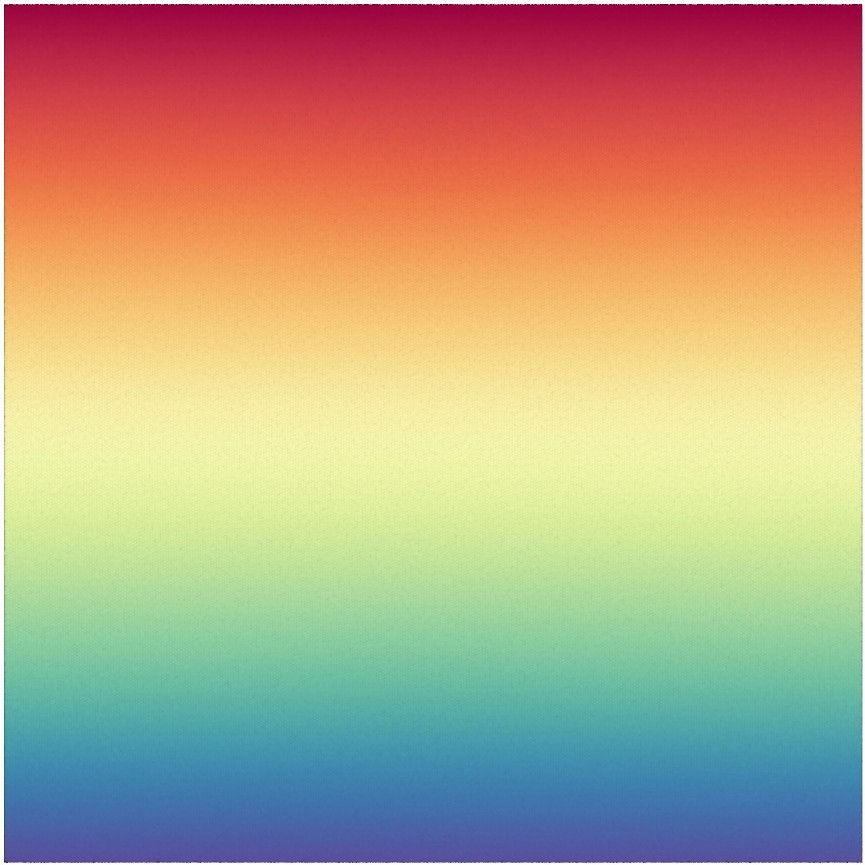
\includegraphics[width=\textwidth]{images/density/taylorgreen_t0.jpg}
    \caption{$t=0s$}
  \end{subfigure}
  \begin{subfigure}[t]{0.4\textwidth}
    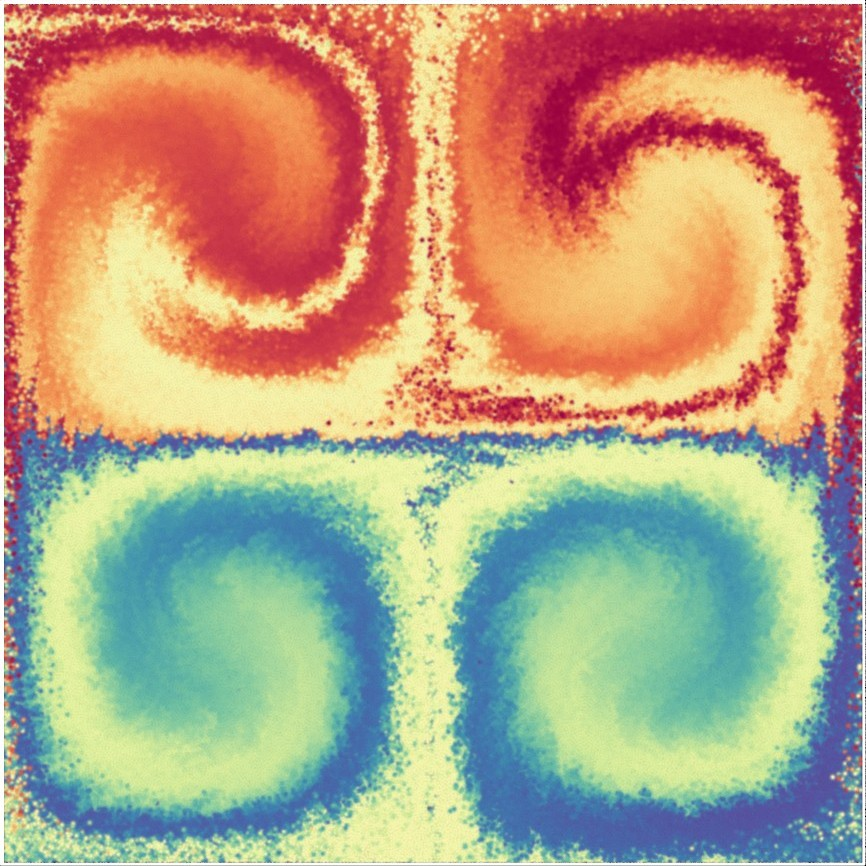
\includegraphics[width=\textwidth]{images/density/taylorgreen_t4_70.jpg}
    \caption{$t=4.7s$}
  \end{subfigure}
  \caption{$95 500$ colour coded particles are advected by a Taylor-Green vortex on a $[0;2\pi]$ domain, with four vertices each spinning in directions opposite to their respectivly adjacent vortices.}
  \label{fig:taylor-green-vortex}
\end{figure}

The rate at which the velocity of the Taylor-Green vortex on a periodic domain decays in relation to the viscosity of a fluid is analytically known to be in $\mathcal{O}br{e^{-\nu t}}$\autocite*{taylor-green-arxiv}. Despite this instance not exactly being a Taylor-Green vortex and the exact analytic solution not holding, the scenario still allows the comparison of decay of the average kinetic energy in the system for different initial samplings of the fluid, where a slower decay is more desireable in reaching lower effective viscosities. A $\frac{1}{N}E_{kin}(t)$ curve can be plotted for different initial sampling lattices and amounts of jitter in conjunction with uniform initial density, as seen in \autoref{fig:taylor-green-result}


\begin{figure}
  \centering
  \includegraphics*[width=\textwidth]{images/density/taylor-green-results.png}
  \caption*{\begin{tiny}$\nu=\nu_2=0, k=1000, \lambda=0.1, N=90500K, \vec{x}\in[0;2\pi]^2, v_{x_0} = 2\sin (x)\cos (y), v_{y,0} = -2\cos (x)\sin (y), \rho_0 = 1$ \texttt{SplitSPH}\end{tiny}}
  \caption{Time evolution of $E_{kin}$ in Taylor-Green vortex for varying amounts of initial jitter and initial sampling lattices. As the initial Jitter approaches a standard deviation of 5\% of the particle spacing, there is a continuous decrease in undesired viscosity. The hexagonal lattice being the most stable in many a sense is detrimental in this case, where to achieve low viscosities, a small jitter and a initial square-lattice sampling seem more effective.}
  \label{fig:taylor-green-result}
\end{figure}

\begin{samepage}


  \autoref{fig:taylor-green-result} suggests that viscosity does in fact decrease as the mass density varies more intensly, at least up to a reasonable amount of initial jitter.
  In order to empirically examine whether this is actually due to fewer rigid, crystalline structures forming, a metric for the degree of crystallinity or amourphousness of a material is required. For this, a metric from the study of two-dimensional melting in condensed matter physics may be borrowed: the Nelson-Halperin 2D bond orientational order parameter\autocite*{bond-orientational-parameter-pis-6} $\Psi_6$. It is defined as\autocite{nicer-psi-6-bond-orientational}:
  \begin{equation}
    \Psi_6^k = \frac{1}{6} \sum_{l\in\mathcal{N}(k)}e^{6i\Theta_{k,l}}
  \end{equation}
  where the sum is over the six nearest neighbours $k\neq l$ to the particle of index $k$, $\Theta_{k,l}$ is the angle between particles $k,l$ measured from an arbitrary, fixed axis and the index $i$ was avoided to not cause confusion with the imaginary unit in the exponent \autocite*{nicer-psi-6-bond-orientational}. Basically, crystals mostly form in hexagonal lattices in two dimensions since in this dimensionality, it is the unique closest packing - how close to crystalline a material is can therefore be measured by how close on average the angles between neighbouring particles are to forming a hexagon. The value $0 \leq \abs{\Psi_6} \leq 1$ is maximized for a hexagonal grid and decreases as the material becomes less 'well-packed'\autocite*{nicer-psi-6-bond-orientational}.

  If there was a relation between jittered masses, lower viscosity and preventing crystal structures, one would expect the average magnitude of the bond orientation parameter $\Psi_6^{avg} = \frac{1}{N}\sum_i \abs{\Psi_6^i}$ to decrease as the jitter increases and the material becomes more disorderly. To test this, $\Psi_6^{avg}$ was measured at $t=30$ for all of the configurations in \autoref{fig:taylor-green-result}, as long as possible after the initialization:

  \begin{center}
    \begin{tabular}{|c | c || c|}
      \hline
      Lattice   & Jitter $\sigma$ & $\Psi_6^{avg}$ \\ [0.5ex]
      \hline\hline
      Hexagonal & 0               & 0.522          \\\hline
      Hexagonal & 0.01h           & 0.511          \\\hline
      Hexagonal & 0.05h           & 0.459          \\\hline
      Square    & 0.01h           & 0.478          \\\hline
      Square    & 0.05h           & 0.444          \\\hline
    \end{tabular}
  \end{center}
\end{samepage}

As can be seen, irrespective of which lattice is used to sample the fluid, there are more defects, less order and therefore lower values of $\Psi_6^{avg}$ as the jitter increases, even long after the initial conditions should have no more bearing on the behaviour of the fluid.

In sources on melting of condensed matter in two dimensions, the hexatic phase is discussed, creating a middle ground between the solid and liquid phases and bearing a surface-level resemblance to structures as seen in \autoref{fig:natural-hexagons} - it might be interesting to draw from knowledge about these physical processes in order to combat undesired visocsity in SPH fluid simulation and reach higher Reynolds numbers, analysing for example the time evolution of translational and orientational order throughout a simulation and how masses and kernel support radii that vary per particle or resampling of fields can influence these phenomena - however those analyses are not conducted in this report.

Instead of focusing on $\Psi_6$ as a metric, the Vornoi tesselation of the particle configuration could also be analysed, counting for example the distribution of particles with five, six or seven nearest neighbours - generally, more amorphous structures that may better physically represent a fluid would be expected to less often have a hexagon as their associated Vornoi cell. On the other hand, especially for small kernel support radii, the SPH approximation quality might suffer from excessive particle disorder.


\chapter{Analysis}\label{chp:analysis}

Having derived the governing equations, discretized them, established initial conditions, boundary conditions and solvers that propagate solutions through time, the description of the implemented solvers has concluded and what is left to discuss is the impact of some design choices made along the way. In particular, the impact of non-uniform masses on the behaviour of the fluid will be discussed in the following, as well as the oscillation that results from having chosen density invariance as the source term for pressure computations. Lastly, the stability of the simulation is discussed in terms of the stiffness parameter $k$ that has been left unspecified, as well as time step size and viscosity.


\section{Impact of Jittered Masses on Viscosity and Structure}

A particularly interesting observation that ties the topic of lattices, random jitter and uniform densities together is the fact that for a uniform initial density combined with a jitter, the mass of the particles is necessarily non-uniform and varies pseudo-randomly. This actually appears to lead to defects in the formation of the crystalline structures that otherwise naturally form, as seen in \autoref{fig:natural-hexagons}, resulting instead in a more amorphous structure. This could have desirable effects, such as increasing isotropy or perhaps reducing undesired viscosity. Intuitively, a particle in a crystalline structure may be expected to require more energy to be moved along an arbitrary direction, than if it had settled into a less rigid structure.

To test this hypothesis, a scene very similar to the Taylor-Green vortex was used, where fluid is initialized at rest density using some lattice as described above, but given a varying degree of pseudo-random jitter in the initial positions. The fluid is contained in a box with no gravity, where all viscosities are in this case set to zero in order to measure only the undesired loss in kinetic energy inherent to the simulation method. The particles are initialized with a velocity that varies according to a sine and cosine function of initial positions $\vek{x}_i(t_0)$ such that four opposing vortices form in each of the four quadrants of a $[0;2\pi]^2$ domain, using in this case\autocite*{taylor-green-arxiv}:

\begin{equation}
  \vek{v}(t=0)_i = 2\begin{pmatrix}
    \sin(x_i) \cos(y_i) \\
    -\cos(x_i) \sin(y_i)
  \end{pmatrix}
\end{equation}
where $\vek{x}_i(t_0) = (x_i, y_i)^T$. The setting is visualized in \autoref{fig:taylor-green-vortex}, where colour-coded particles are advected.

\begin{figure}
  \centering
  \begin{subfigure}[t]{0.4\textwidth}
    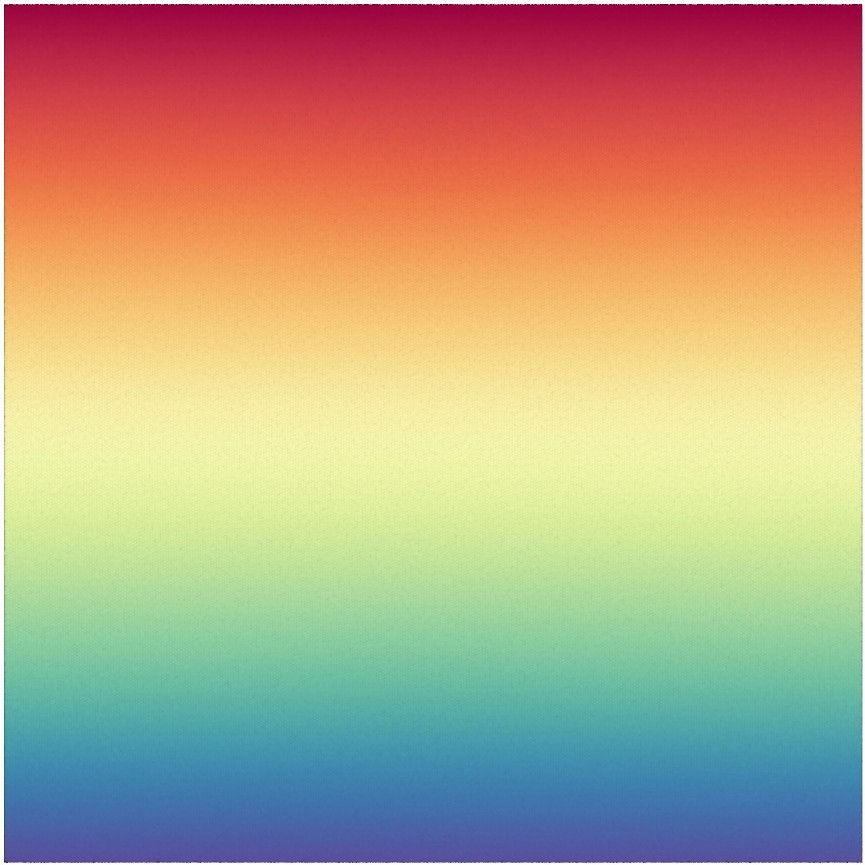
\includegraphics[width=\textwidth]{images/density/taylorgreen_t0.jpg}
    \caption{$t=0s$}
  \end{subfigure}
  \begin{subfigure}[t]{0.4\textwidth}
    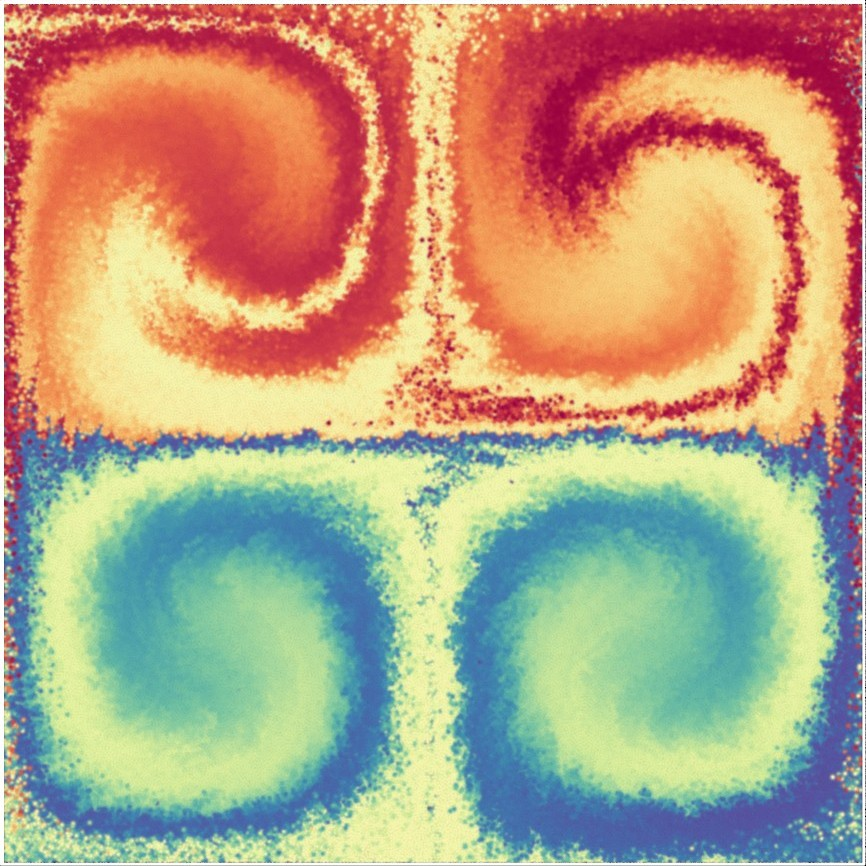
\includegraphics[width=\textwidth]{images/density/taylorgreen_t4_70.jpg}
    \caption{$t=4.7s$}
  \end{subfigure}
  \caption{$95 500$ colour coded particles are advected by a Taylor-Green vortex on a $[0;2\pi]$ domain, with four vertices each spinning in directions opposite to their respectively adjacent vortices.}
  \label{fig:taylor-green-vortex}
\end{figure}

The rate at which the velocity of the Taylor-Green vortex on a periodic domain decays in relation to the viscosity of a fluid is analytically known to be\autocite*{taylor-green-arxiv} in $\mathcal{O}\br{e^{-\nu t}}$. Despite the exact analytic solution not holding in this instance since periodic boundaries are not applied, the scenario still allows the comparison of decay of the average kinetic energy in the system for different initial samplings of the fluid, where a slower decay is more desirable in reaching lower effective viscosities. A $\frac{1}{N}E_{kin}(t)$ curve can be plotted for different initial sampling lattices and amounts of jitter in conjunction with uniform initial density as described in \autoref{sec:equilibrate-density}, which is shown in \autoref{fig:taylor-green-result}


\begin{figure}
  \centering
  \begin{tikzpicture}
    \begin{axis}[
      xlabel={Time $t$},
      ylabel={Average Kinetic Energy $\frac{1}{N}E_{kin}(t)$},
      legend pos=south west,
      legend style={font=\small, cells={anchor=west}}, % Make legend smaller and more compact
      grid=none,
      no markers,
      every axis plot/.append style={ultra thin},
      axis line style={-},
      tick align=outside,
      tick style={thin, black},
      clip=false,
      enlarge x limits=0, % remove padding
      enlarge y limits=0, % remove padding
      width=\textwidth
      ]

      \addplot [color=Spectral0] table [x=hex_0jitterx, y=hex_0jittery, col sep=comma] {taylor_avg_ekin_over_t.csv};
      \addlegendentry{Hexagonal Lattice, $\sigma=0h$}

      \addplot [color=Spectral1] table [x=hex_1jitterx, y=hex_1jittery, col sep=comma] {taylor_avg_ekin_over_t.csv};
      \addlegendentry{Hexagonal Lattice, $\sigma=0.01h$}

      \addplot [color=Spectral2] table [x=hex_5jitterx, y=hex_5jittery, col sep=comma] {taylor_avg_ekin_over_t.csv};
      \addlegendentry{Hexagonal Lattice, $\sigma=0.05h$}

      \addplot [color=Spectral3] table [x=reg_1jitterx, y=reg_1jittery, col sep=comma] {taylor_avg_ekin_over_t.csv};
      \addlegendentry{Square Lattice, $\sigma=0.01h$}

      \addplot [color=Spectral4] table [x=reg_5jitterx, y=reg_5jittery, col sep=comma] {taylor_avg_ekin_over_t.csv};
      \addlegendentry{Square Lattice, $\sigma=0.05h$}

    \end{axis}
  \end{tikzpicture}

  \caption*{\begin{tiny}$\nu=\nu_2=0, k=1000, h=0.033, \lambda=0.1, N=90500K, \vec{x}\in[0;2\pi]^2, v_{x_0} = 2\sin (x)\cos (y), v_{y,0} = -2\cos (x)\sin (y), \rho_0 = 1$ \texttt{SplitSPH}\end{tiny}}
  \caption{Time evolution of $\frac{1}{N}E_{kin}$ in Taylor-Green vortex for varying amounts of initial jitter and initial sampling lattices. As the initial Jitter approaches a standard deviation of 5\% of the particle spacing $h$, there is a continuous decrease in undesired viscosity. The hexagonal lattice being the most stable in many a sense is detrimental in this case, where to achieve low viscosities, a small jitter and an initial square-lattice sampling appear more effective.}
  \label{fig:taylor-green-result}
\end{figure}



\begin{samepage}


  \autoref{fig:taylor-green-result} suggests that viscosity does in fact decrease as the mass varies more intensely, at least up to a reasonable amount of initial jitter.
  In order to empirically examine whether this is actually due to fewer rigid, crystalline structures forming, a metric for the degree of crystallinity or amorphousness of a material, or in other words a structural order parameter, is required. For this, a metric from the study of two-dimensional melting in condensed matter physics may be borrowed: the Nelson-Halperin 2D bond orientational order parameter\autocite*{bond-orientational-parameter-pis-6} $\Psi_6$. It is defined as\autocite{nature-psi-6-bond-orientational}:
  \begin{equation}
    \Psi_6^k = \frac{1}{n_k} \sum_{l\in\mathcal{N}(k)}e^{6i\Theta_{k,l}}
  \end{equation}
  where the sum is over the $n_k$ nearest neighbours $k\neq l$ to the particle of index $k$ determined through a Delaunay triangulation, $\Theta_{k,l}$ is the angle between particles $k,l$ measured from an arbitrary, fixed axis and the usual particle index $i$ was avoided to not cause confusion with the imaginary unit in the exponent \autocite*{nature-psi-6-bond-orientational}. Generally, the $\Psi_x$ metric shows how close to perfect $x$-atic symmetry the local environment is, which is why the hexatic $\Psi_6$ metric was chosen for this two-dimensional case where the hexagon is the unique closest packing and six nearest neighbours are indeed the most frequent result of a Delaunay triangulation of the particle positions for all simulation runs. The value $0 \leq \abs{\Psi_6} \leq 1$ is maximized for a hexagonal grid and decreases as the material becomes less ordered\autocite*{nature-psi-6-bond-orientational}, where magnitude expresses regularity or how 'well-packed' the arrangement is\autocite*{nicer-psi-6-bond-orientational}, while the complex number itself also encodes a phase or orientation of the structure.

  If there was a relation between jittered masses, lower viscosity and preventing crystal structures, one would expect the average magnitude of the bond orientation parameter $\Psi_6^{avg} = \frac{1}{N}\sum_i \abs{\Psi_6^i}$ to decrease as the jitter increases and the material becomes more disorderly. To test this, $\Psi_6^{avg}$ was measured at $t=30$ for all the configurations in \autoref{fig:taylor-green-result}, long after the initialization, with results shown in table \ref{tbl:hexatic-order}.

  \begin{figure}[H]
    \begin{center}
      \begin{tabular}{|c | c | c || c|}
        \hline
        Lattice   & Time & Jitter $\sigma$ & $\Psi_6^{avg}$ \\
        \hline\hline
        Hexagonal & t=0  & 0               & 0.973          \\\hline
        Hexagonal & t=30 & 0               & 0.522          \\\hline
        Hexagonal & t=30 & 0.01h           & 0.511          \\\hline
        Hexagonal & t=30 & 0.05h           & 0.459          \\\hline
        Square    & t=30 & 0.01h           & 0.478          \\\hline
        Square    & t=30 & 0.05h           & 0.444          \\\hline
      \end{tabular}
      \caption{The average bond orientational parameter $\Psi_6^{avg}$ is shown for different initial samplings and amounts of jitter. The $t=0$ entry highlights how a hexagonal structure maximizes this value, while increasing jitter results in lower values, even at $t=30$.}
      \label{tbl:hexatic-order}
    \end{center}
  \end{figure}
\end{samepage}


As can be seen, irrespective of which lattice is used to sample the fluid, there are more defects, less order and therefore lower values of $\Psi_6^{avg}$ as the jitter increases, even long after the initial conditions should have no more bearing on the behaviour of the fluid. This further suggests that the combination of jitter and solving for uniform density could indeed make the discretization more isotropic and help decrease unwelcome viscosity. On the other hand, especially for small kernel support radii, the SPH approximation quality might suffer from excessive particle disorder.

Just to further drive home the point that order decreases as particle masses vary, the Voronoi tessellations of the particle positions from the same simulation runs can be analysed instead of $\Psi_6$. Then, particles the Vornoi cells of which form a polygon with six vertices, more than six or less than six vertices can be coloured respectively and plotted, as seen in \autoref{fig:jitter-vornoi-tesselation}. This again suggests that jittered masses lead to more defects in otherwise locally ordered structures.

\begin{figure}
  \begin{subfigure}[t]{0.49\textwidth}
    \includegraphics[width=\textwidth]{images/density/hex_0jitter_vornoi.png}
    \caption{$\sigma=0$}
  \end{subfigure}
  \begin{subfigure}[t]{0.49\textwidth}
    \includegraphics[width=\textwidth]{images/density/hex_5jitter_vornoi.png}
    \caption{$\sigma=0.05h$}
  \end{subfigure}
  \caption{The result of the Vornoi tessellation of the simulations of the Taylor-Green vortex are shown for a hexagonal initial sampling at $t=30$ with the specified jitter (all parameters are the same as in \autoref{fig:taylor-green-result}). Each particle that has a Voronoi cell with more than six vertices is coloured red, ones with fewer neighbours are coloured green. While for  $\sigma=0$, there are 61759 particles that have hexagonal Voronoi cells, for $\sigma=0.05h$ jitter there are only 52845 such particles, as can be seen observed in the increased amount of coloured dots in the right figure. This further suggests that pseudo-randomly varying particle masses create a less ordered and possibly more isotropic structure down the line.}
  \label{fig:jitter-vornoi-tesselation}
\end{figure}

In sources on melting of condensed matter in two dimensions, the hexatic phase is frequently examined, creating a continuous middle ground between the solid and liquid phases and bearing a surface-level resemblance to the structures seen in \autoref{fig:natural-hexagons} - it might be interesting to draw from knowledge about these physical processes in order to combat undesired viscosity in SPH fluid simulation and reach higher effective Reynolds numbers, analysing for example the time evolution of translational and orientational order throughout a simulation and how masses and kernel support radii that vary per particle or resampling of fields can influence these phenomena - however those analyses are not conducted in this report.


\newpage
\section{Oscillation Frequency and Error as a Function of Stiffness}\label{sec:oscillations}
By choosing a density invariance term in the formulation of the fluid solvers instead of the velocity divergence, the fluid can be expected to oscillate about its rest density for the non-iterative solvers \texttt{SplitSPH} and \texttt{EOSSPH} instead of exhibiting volume drift.


The iterative solver behaves somewhat similarly, but does not oscillate about the rest density in a sinusoidal fashion since incompressibility is more strongly enforced with a density error threshold that the average density does not significantly exceed, resulting in peaks of the oscillations in density being cut off. To make the \texttt{IterSPH} solver more comparable, a fixed amount of iterations can be used, $l=l_{min}=l_{max}=3$ and $l=2$ respectively in this case, which makes the oscillation regular but disables any error thresholds or guarantees.

One can analyse the behaviour of this oscillating error using a simple column of water in a tall, rectangular container, since it is known that this configuration would ideally result in a perfectly still fluid that does not oscillate. The width of the container has little bearing on the magnitude of the error, which is why a narrow and tall configuration is preferred in order to analyse the same effect using fewer particles and therefore less computation time. Both the amplitude and the frequency of this oscillation can be found to depend on the stiffness parameter $k$ that governs incompressibility in the equation of state. In this section, the influence of $k$ on the magnitude of the error and the frequency of the oscillation are analysed. The setting and the oscillation are shown in \autoref{fig:oscillating-column}

\begin{figure}[h]
  \centering
  \begin{subfigure}[t]{0.09\textwidth}
    
\includegraphics[width=\textwidth]{images/oscillate/000.jpg}
    \caption{\small{$t=0.0s$}}
  \end{subfigure}%
  \begin{subfigure}[t]{0.09\textwidth}
    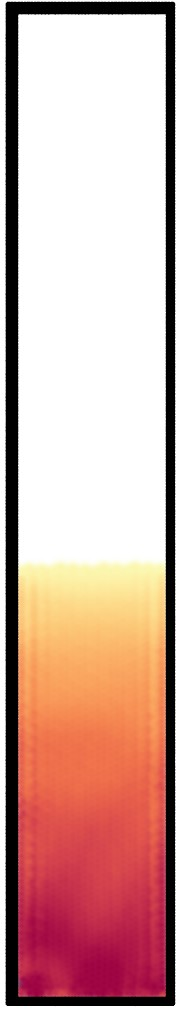
\includegraphics[width=\textwidth]{images/oscillate/020.jpg}
    \caption{\small{$t=0.2s$}}
  \end{subfigure}%
  \begin{subfigure}[t]{0.09\textwidth}
    
\includegraphics[width=\textwidth]{images/oscillate/030.jpg}
    \caption{\small{$t=0.3s$}}
  \end{subfigure}%
  \begin{subfigure}[t]{0.09\textwidth}
    
\includegraphics[width=\textwidth]{images/oscillate/040.jpg}
    \caption{\small{$t=0.4s$}}
  \end{subfigure}%
  \begin{subfigure}[t]{0.09\textwidth}
    
\includegraphics[width=\textwidth]{images/oscillate/050.jpg}
    \caption{\small{$t=0.5s$}}
  \end{subfigure}%
  \begin{subfigure}[t]{0.09\textwidth}
    
\includegraphics[width=\textwidth]{images/oscillate/060.jpg}
    \caption{\small{$t=0.6s$}}
  \end{subfigure}%
  \begin{subfigure}[t]{0.09\textwidth}
    
\includegraphics[width=\textwidth]{images/oscillate/070.jpg}
    \caption{\small{$t=0.7s$}}
  \end{subfigure}%
  \begin{subfigure}[t]{0.09\textwidth}
    
\includegraphics[width=\textwidth]{images/oscillate/080.jpg}
    \caption{\small{$t=0.8s$}}
  \end{subfigure}%
  \begin{subfigure}[t]{0.09\textwidth}
    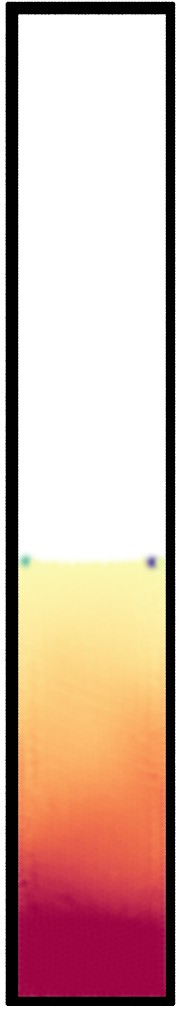
\includegraphics[width=\textwidth]{images/oscillate/090.jpg}
    \caption{\small{$t=0.9s$}}
  \end{subfigure}%
  \begin{subfigure}[t]{0.09\textwidth}
    
\includegraphics[width=\textwidth]{images/oscillate/100.jpg}
    \caption{\small{$t=1.0s$}}
  \end{subfigure}
  \caption*{\begin{tiny}$k=100, \nu=0.01, \nu_2=0, h=0.02, \lambda=0.1, N=1572, \rho_0 = 1, \Delta t = 0.0002s$ \texttt{SplitSPH}\end{tiny}}
  \caption{A half-filled, tall, rectangular tube is shown with the density of the fluid being colour-coded. For the very small stiffness parameter $k=100$ shown here, major compressions occur and a clearly visible, slow oscillation sets in.}
  \label{fig:oscillating-column}
\end{figure}

The effect can be thought of as an oscillation due to the fact that particles at the top of the column are still in free fall when the bottom particles first experience contact forces - the stiffer the fluid, the faster the shock within it propagates and the quicker the particles at the top of the column are accelerated back up, where gravity takes over and the cycle continues, albeit with smaller and smaller amplitude.

In order to conduct the analysis, the measured density according to \autoref{eq:density-sph} can be averaged across all particles to obtain $\rho_{avg}(t) = \frac{1}{N}\sum_i \rho_i(t)$, and the rest density subtracted to obtain the average density error $\Delta \rho(t) = \rho_{avg}(t)-\rho_0$, which ideally oscillates about zero. This is done for a simulation running with a specified, fixed time step $\Delta t$; the CFL-condition is not used in favour of obtaining a regular sampling of the $\Delta \rho(t)$-Curve which can be more easily subjected to a discrete Fourier transform to analyse the frequency of the oscillation. In the following, a time step size of $\Delta t = 0.0002s$ is used, which is a conservative estimate of the $\Delta t$ required by the CFL condition. This means that $\Delta \rho(t)$ is sampled at $5000Hz$ and the frequency:
\begin{equation}
  f_{peak}=\argmax_{f}\mathcal{F}\br{\Delta \rho(t)} = \argmax_{f}\Delta\rho'(f)
\end{equation}
with maximum contribution to the spectrum of the oscillation is plotted against $k$, neglecting the zero-frequency $f_0$ which is plotted in a separate graph and expresses the magnitude of the total error. This is done for $2s\leq t\leq 12s$, where the first two seconds of simulated time are discarded in order to minimize the impact of the initial configuration.

\begin{figure}[hbt]
  \begin{tikzpicture}
    \begin{axis}[
        xlabel={Stiffness $k$},
        ylabel={Peak oscillation frequency $f_{peak} (Hz)$},
        legend pos=north west,
        legend style={font=\small, cells={anchor=west}}, % Make legend smaller and more compact
        grid=none,
        no markers,
        every axis plot/.append style={ultra thin},
        axis line style={-},
        tick align=outside,
        tick style={thin, black},
        clip=false,
        enlarge x limits=0, % remove padding
        enlarge y limits=0, % remove padding
        width=\textwidth,
        height=0.7\textwidth,
        % xmode=log,
        % ymode=log,
      ]

      \addplot [color=Spectral2, thick] table [x=k, y=EOSSPHhighvis, col sep=comma] {k_to_freq.csv};
      \addlegendentry{\texttt{EOSSPH}, $\nu=10^{-2}$}
      \addplot [color=Spectral3, dashed] table [x=k, y=EOSSPHlowvis, col sep=comma] {k_to_freq.csv};
      \addlegendentry{\texttt{EOSSPH}, $\nu=10^{-3}$}

      \addplot [color=black, thick, dotted] table [x=k, y=SplitSPHhighvis, col sep=comma] {k_to_freq.csv};
      \addlegendentry{\texttt{SplitSPH}, $\nu=10^{-2}$}
      % \addplot [color=Spectral5, dashed] table [x=k, y=SplitSPHlowvis, col sep=comma] {k_to_freq.csv};
      % \addlegendentry{\texttt{SplitSPH}, $\nu=10^{-3}$}

      \addplot [color=Spectral6, thick] table [x=k, y=IterSPHhighvis2, col sep=comma] {k_to_freq.csv};
      \addlegendentry{\texttt{IterSPH}, $l=2,\nu=10^{-2}$}
      % \addplot [color=Spectral7, dashed] table [x=k, y=IterSPHlowvis2, col sep=comma] {k_to_freq.csv};
      % \addlegendentry{\texttt{IterSPH}, $l=2,\nu=10^{-3}$}

      \addplot [color=Spectral8, thick] table [x=k, y=IterSPHhighvis, col sep=comma] {k_to_freq.csv};
      \addlegendentry{\texttt{IterSPH}, $l=3,\nu=10^{-2}$}
      % \addplot [color=Spectral10, dashed] table [x=k, y=IterSPHlowvis, col sep=comma] {k_to_freq.csv};
      % \addlegendentry{\texttt{IterSPH}, $l=3,\nu=10^{-3}$}

      \addplot [color=red] table [x=k, y=prediction, col sep=comma] {k_to_freq.csv};
      \addlegendentry{Prediction $l=3$ }
      \addplot [color=red, dashed] table [x=k, y=prediction2, col sep=comma] {k_to_freq.csv};
      \addlegendentry{Prediction $l=2$ }

    \end{axis}
  \end{tikzpicture}
  \caption*{\begin{tiny}$\nu_2=0.001, h=0.02, \Delta t = 0.0002s, N=1572, \rho_0 = 1, \gamma_1=1, \gamma_2=0.5$, Hexagonal sampling with $\sigma=0.015h$\end{tiny}}
  \caption{The frequency $f_{peak}$ with maximum contribution to the oscillation of the function $\Delta\rho (t)$ is plotted against the stiffness parameter $k$ that governs incompressibility. The frequency of oscillation continuously increases as $k$ increases. The curves of the \texttt{EOSSPH} and \texttt{SplitSPH} simulations all overlap and so do all curves that differ only in viscosity, so only a selection of such curves was plotted.}
  \label{fig:freq-peak-k}
\end{figure}

The results of the frequency analysis are shown in \autoref{fig:freq-peak-k}.
This graph shows that as the stiffness $k$ increases, so does the frequency of the oscillation. The graph closely resembles a square root function, which might be explained by the stiffness being linked to the \emphasis{numerical speed of sound} $c$, which governs the frequency of the oscillations\autocite*{speed-of-sound-k}, through the Newton-Laplace equation that states\autocite*{speed-of-sound}:
\begin{equation}\label{eq:newton-laplace}
  c = \sqrt{\frac{\Delta p}{\Delta\rho}}
\end{equation}
meaning that for the equation of state in \autoref{eq:state-equation} for which $\Delta p \propto k\Delta\rho$ and if the oscillation frequency is indeed proportional to the numerical speed of sound ($f_{peak} \propto c$), then:
\begin{equation}
  f_{peak}
  \propto c
  = \sqrt{\frac{\Delta p}{\Delta\rho}}
  \propto \sqrt{\frac{k \Delta\rho}{\Delta\rho}}
  = \sqrt{k}
\end{equation}
and therefore $f_{peak} \propto \sqrt{k}$, which would explain the shape of the curve.

The graph also clearly shows that the oscillation is \textit{not affected} by viscosity, with simulations that differ in $\nu$ by an order of magnitude exactly overlapping, and that operator splitting \textit{also does not affect} the result at all. This further evidences that the oscillation frequency depends on the numerical speed of sound and not any of the other factors mentioned. The only solver with a differing curve is the iterative solver: for this solver, one would expect the numerical speed of sound to be higher, since there are multiple iterations per time step that may propagate information, or accelerations, from neighbouring particle to neighbouring particle - this makes intuitive sense, since the iterative solver achieves a higher effective incompressibility, which has been shown to be linked to the numerical speed of sound in \autoref{eq:newton-laplace}.


One could speculate that within some low bound of $l_{iter}$, where repeated neighbourhood calculations are not necessary, the number of iterations could have a nearly linear relationship with the stiffness $k$, the square root of which was assumed above to be proportional to the frequency of oscillation - if this were true, one would expect the iterative solver with $l_{iter}=2$ to have a higher frequency of oscillation by a factor of $\sqrt{l_{iter}}=\sqrt{2}$ and similarly for $l=3$.
To test this hypothesis, the average of the four curves using a single-iteration solver as seen in \autoref{fig:freq-peak-k} was taken (\texttt{EOSSPH}, \texttt{SplitSPH} for $\nu=10^{-2}, \nu-10^{-3}$ respectively), a square root function fitted to this average using the Levenberg-Marquardt algorithm for least squares regression\footnote{Implemented in SciPy Optimize: Curve Fit \url{https://docs.scipy.org/doc/scipy/reference/generated/scipy.optimize.curve_fit.html}} and then multiplied by $\sqrt{l_{iter}}$ to yield the red line and dashed red line shown in \autoref{fig:freq-peak-k} as the \textit{Prediction}. These curves describe what would be expected to happen if the hypotheses made in this section were true, meaning:
\begin{enumerate}
  \item $f_{peak}\propto\sqrt{k}$
  \item  $k\propto l_{iter}$
\end{enumerate}
and matches the experimental values for both the $l=2$ and the $l=3$ iterative solvers remarkably well, suggesting that stiffness may indeed be almost linear in the number of iterations for such solvers, at least up to some small, fixed number of iterations.

\horizontalspacer


The total density error across time can be expressed by the zero-frequency $f_0$ of the discrete Fourier transform of $\Delta\rho (t)$ as shown in \autoref{fig:error-to-k}, where:
\begin{equation}
  f_0 = \int_{2s}^{10s} \Delta\rho (t) \,dt
\end{equation}
Note that $\Delta\rho (t)$ should oscillate about zero, so the integral should be zero if the solver perfectly enforces incompressibility, greater than zero if some compression occurs and negative if somehow the measured average density across particles and time is below rest density.

Here, the data shows that a greater stiffness coefficient $k$ results in less density error, which makes sense since compressions for higher $k$ result in greater pressure forces that correct the compression.

The graph also shows how increasing the stiffness $k$ yields diminishing returns, further motivating the use of iterative solvers as a way to improve simulation quality, since simply increasing the stiffness used in a single iteration per time step might become unfeasible. The iterative solver achieves a much smaller value of $f_0$ across all coefficients $k$, with higher iteration counts further decreasing the error, but once again an increase in iteration count appears to yield diminishing returns.

In this instance, the single-iteration solvers with and without operator splitting again show the same behaviour, with viscosity once more playing no role in the oscillation for the measured range of parameters. Operator splitting, while perhaps effective in reducing some kinds of errors and improving robustness and stability, does not have an impact on the type of error under consideration in this scenario.


At some point, when increasing $k$, instability might occur if the time step size $\Delta t$ is not simultaneously decreased, making the simulation more computationally expensive - this is analysed in the following section.


\begin{figure}[hbt]
  \begin{tikzpicture}
    \begin{axis}[
        xlabel={Stiffness $k$},
        ylabel={Zero Frequency $f_{0}$},
        legend pos=north east,
        legend style={font=\small, cells={anchor=west}}, % Make legend smaller and more compact
        grid=none,
        no markers,
        every axis plot/.append style={ultra thin},
        axis line style={-},
        tick align=outside,
        tick style={thin, black},
        clip=false,
        enlarge x limits=0, % remove padding
        enlarge y limits=0, % remove padding
        width=\textwidth,
        height=0.7\textwidth,
        % xmode=log,
        % ymode=log,
      ]

      \addplot [color=Spectral0, thick] table [x=k, y=EOSSPHhighvis, col sep=comma] {k_to_error.csv};
      \addlegendentry{\texttt{EOSSPH}, $\nu=10^{-2}$}
      \addplot [color=Spectral2, dashed] table [x=k, y=EOSSPHlowvis, col sep=comma] {k_to_error.csv};
      \addlegendentry{\texttt{EOSSPH}, $\nu=10^{-3}$}

      \addplot [color=Spectral4, thick] table [x=k, y=SplitSPHhighvis, col sep=comma] {k_to_error.csv};
      \addlegendentry{\texttt{SplitSPH}, $\nu=10^{-2}$}
      \addplot [color=Spectral6, dashed] table [x=k, y=SplitSPHlowvis, col sep=comma] {k_to_error.csv};
      \addlegendentry{\texttt{SplitSPH}, $\nu=10^{-3}$}


      \addplot [color=Spectral7, thick] table [x=k, y=IterSPHhighvis2, col sep=comma] {k_to_error.csv};
      \addlegendentry{\texttt{IterSPH}, $l=2,\nu=10^{-2}$}
      \addplot [color=Spectral8, dashed] table [x=k, y=IterSPHlowvis2, col sep=comma] {k_to_error.csv};
      \addlegendentry{\texttt{IterSPH}, $l=2,\nu=10^{-3}$}

      \addplot [color=Spectral9, thick] table [x=k, y=IterSPHhighvis, col sep=comma] {k_to_error.csv};
      \addlegendentry{\texttt{IterSPH}, $l=3,\nu=10^{-2}$}
      \addplot [color=Spectral10, dashed] table [x=k, y=IterSPHlowvis, col sep=comma] {k_to_error.csv};
      \addlegendentry{\texttt{IterSPH}, $l=3,\nu=10^{-3}$}

    \end{axis}
  \end{tikzpicture}
  \caption*{\begin{tiny}$\nu_2=0.001, h=0.02, \Delta t = 0.0002s, N=1572, \rho_0 = 1, \gamma_1=1, \gamma_2=0.5$, Hexagonal sampling with $\sigma=0.015h$\end{tiny}}
  \caption{The zero frequency $f_0$ or integral of the function $\Delta\rho (t)$ is plotted against the stiffness parameter $k$ that governs incompressibility. As the stiffness increases, the total error sharply decreases. The viscosity and whether operator splitting is applied has no impact on the single-iteration solvers \texttt{EOSSPH} and \texttt{SplitSPH}, the curves of which all overlap. The \texttt{IterSPH} solver with achieves a lower total error across all $k$, with higher iteration counts resulting in lower errors but seemingly yielding diminishing returns.}
  \label{fig:error-to-k}
\end{figure}

\newpage

\section{Stability as a Function of Viscosity, Stiffness and Time Step Size}
The setting described in \autoref{sec:oscillations}, where a column of water at rest is simulated, can also be used to analyse the stability of the simulation. Once again, the fact that the water ought to be at rest and therefore the analytic solution is trivially known can be used to measure an error $\epsilon$ relative to that solution for each of the solvers presented in \autoref{chp:solvers}. It has already been discussed that higher stiffness $k$ can lead to better simulation accuracy, but it has not yet been shown that a choice of $k$ that is too large for a given time step size $\lambda$ can lead to unstable behaviour with erratically moving particles and unphysical behaviour. Ideally, the average kinetic energy of the fluid particles $E_{kin}(t) = \frac{1}{N}\sum_i m_i \dist{\vek{v}_i(t)}^2$ is at zero, or very close to it, for the resting water column shown in \autoref{fig:oscillating-column}. Instabilities can be detected by the kinetic energy being considerably higher than expected and repeatedly spiking, which is measured in the following using the logarithm of the average time integral of kinetic energy of the particles, or assuming a potential energy of zero, the logarithm of the average action:
\begin{equation}\label{eq:action-log-error}
  \epsilon = \log_{10}\br{\int_{10s}^{20s} E_{kin}(t) \,dt}
\end{equation}
where the first 10 seconds are discarded to make sure that any movement due to unfortunate initial conditions and the oscillations measured in \autoref{sec:oscillations} have subsided, the state of the particles is somewhat equilibrated, and instabilities are responsible for any remaining, significant amounts of kinetic energy. The time integration in \autoref{eq:action-log-error} is implemented using the trapezoidal rule and the logarithm is taken to account for an unstable simulation potentially having multiple orders of magnitude more kinetic energy than a stable simulation in this scenario. The scenario for one set of parameters and varying solvers is shown in \autoref{fig:stability-increasing}, while the results of the analysis are shown in \autoref{fig:stability-k-lambda}.


\begin{figure}[h]
  \centering
  \begin{subfigure}[t]{0.1\textwidth}
    \centering
    \includegraphics*[width=\textwidth]{images/stability/eos.jpg}
    \caption{\small{\texttt{EOSSPH}}}
  \end{subfigure}
  \hspace*{0.1\textwidth}
  \begin{subfigure}[t]{0.1\textwidth}
    \centering
    \includegraphics*[width=\textwidth]{images/stability/split.jpg}
    \caption{\small{\texttt{SplitSPH}}}
  \end{subfigure}
  \hspace*{0.1\textwidth}
  \begin{subfigure}[t]{0.1\textwidth}
    \centering
    \includegraphics*[width=\textwidth]{images/stability/iter.jpg}
    \caption{\small{\texttt{IterSPH}}}
  \end{subfigure}

  \caption*{\begin{tiny}$\lambda=0.1, \nu=0.0001, \nu_2=0.001, h=0.02, N=1572, \rho_0 = 1, \gamma_1=1, \gamma_2=0.5$, Hexagonal sampling with $\sigma=0.015h$\end{tiny}}
  \caption{The exact same setting with the same parameters is shown at $t=5s$ for different solvers, showcasing how operator splitting can increase stability and the iterative solver further improves this. The magnitudes of velocities are colour-coded.}
  \label{fig:stability-increasing}
\end{figure}


\begin{figure}
  \centering
  \begin{subfigure}[t]{\textwidth}
    \centering
    \begin{tikzpicture}
      \begin{groupplot}[
          group style={
              group size=2 by 3,
              vertical sep=2cm,
              horizontal sep=2cm,
            },
          colormap name=Spectral_r,
          % colormap/viridis, 
          point meta min=-1.9,
          point meta max=2.1,
          view={0}{90},
          xlabel={$k$},
          ylabel={$\lambda$},
          zlabel={$\epsilon$},
          width=0.45\textwidth,
          height=0.45\textwidth,
        ]
        \nextgroupplot[
          title={\texttt{EOSSPH}}
        ]

        \addplot3 [
          contour filled,
        ] table {500.0 0.1 -1.775406581727304
500.0 0.325 -1.774586966838677
500.0 0.55 -1.774586966838677
500.0 0.775 -1.774586966838677
500.0 1.0 -1.774586966838677

750.0 0.1 -1.0878262651867756
750.0 0.325 -1.5754976317756555
750.0 0.55 -1.5754976317756555
750.0 0.775 -1.5754976317756555
750.0 1.0 -1.5754976317756555

1000.0 0.1 0.264343272412918
1000.0 0.325 1.1789164093276245
1000.0 0.55 1.5611023545911076
1000.0 0.775 1.347344268713195
1000.0 1.0 1.6559787819070602

1250.0 0.1 0.3461347056438925
1250.0 0.325 1.2782060111110884
1250.0 0.55 1.6633369289893745
1250.0 0.775 1.4517300660877828
1250.0 1.0 1.9622149802043296

1500.0 0.1 0.3989528205702097
1500.0 0.325 1.3463315307193444
1500.0 0.55 1.7450584697134934
1500.0 0.775 1.5413034002108208
1500.0 1.0 2.070669817702054

};

        \addplot3 [
          contour gnuplot={
              contour dir=z,
              levels={-2,-1.5,-1,-0.5,0,0.5,1,1.5,2},
              labels over line,
              draw color = black,
            },
          thick,
        ] table {500.0 0.1 -1.775406581727304
500.0 0.325 -1.774586966838677
500.0 0.55 -1.774586966838677
500.0 0.775 -1.774586966838677
500.0 1.0 -1.774586966838677

750.0 0.1 -1.0878262651867756
750.0 0.325 -1.5754976317756555
750.0 0.55 -1.5754976317756555
750.0 0.775 -1.5754976317756555
750.0 1.0 -1.5754976317756555

1000.0 0.1 0.264343272412918
1000.0 0.325 1.1789164093276245
1000.0 0.55 1.5611023545911076
1000.0 0.775 1.347344268713195
1000.0 1.0 1.6559787819070602

1250.0 0.1 0.3461347056438925
1250.0 0.325 1.2782060111110884
1250.0 0.55 1.6633369289893745
1250.0 0.775 1.4517300660877828
1250.0 1.0 1.9622149802043296

1500.0 0.1 0.3989528205702097
1500.0 0.325 1.3463315307193444
1500.0 0.55 1.7450584697134934
1500.0 0.775 1.5413034002108208
1500.0 1.0 2.070669817702054

};
        \nextgroupplot[
          title={\texttt{EOSSPH}},
          view={60}{30},
          x dir=reverse,
          zmin=-1.9,
          zmax=2.1,
          % zlabel={\Epsilon},
        ]
        \addplot3 [
          surf,
          faceted color=black,
        ] table {500.0 0.1 -1.775406581727304
500.0 0.325 -1.774586966838677
500.0 0.55 -1.774586966838677
500.0 0.775 -1.774586966838677
500.0 1.0 -1.774586966838677

750.0 0.1 -1.0878262651867756
750.0 0.325 -1.5754976317756555
750.0 0.55 -1.5754976317756555
750.0 0.775 -1.5754976317756555
750.0 1.0 -1.5754976317756555

1000.0 0.1 0.264343272412918
1000.0 0.325 1.1789164093276245
1000.0 0.55 1.5611023545911076
1000.0 0.775 1.347344268713195
1000.0 1.0 1.6559787819070602

1250.0 0.1 0.3461347056438925
1250.0 0.325 1.2782060111110884
1250.0 0.55 1.6633369289893745
1250.0 0.775 1.4517300660877828
1250.0 1.0 1.9622149802043296

1500.0 0.1 0.3989528205702097
1500.0 0.325 1.3463315307193444
1500.0 0.55 1.7450584697134934
1500.0 0.775 1.5413034002108208
1500.0 1.0 2.070669817702054

};

				% -----------------------------------------------------------------------------------------------
      
        \nextgroupplot[
          title={\texttt{SplitSPH}}
        ]
        \addplot3 [
          contour filled,
        ] table {500.0 0.1 -1.8767772764572803
500.0 0.325 -1.8767772764572803
500.0 0.55 -1.8767772764572803
500.0 0.775 -1.8767772764572805
500.0 1.0 -1.8767772764572805

750.0 0.1 -0.3789489823565821
750.0 0.325 -0.34902458912763246
750.0 0.55 -0.34902458912763246
750.0 0.775 -0.34902458912763246
750.0 1.0 -0.34902458912763246

1000.0 0.1 -0.031326103139639266
1000.0 0.325 0.7029563610938275
1000.0 0.55 1.0375172646519517
1000.0 0.775 1.2558846092107683
1000.0 1.0 1.3978417037016113

1250.0 0.1 0.08853083786483268
1250.0 0.325 0.8935064048810112
1250.0 0.55 1.2264769730234093
1250.0 0.775 1.4545908600522692
1250.0 1.0 1.678435080159394

1500.0 0.1 0.16427613556411932
1500.0 0.325 0.9709248573056103
1500.0 0.55 1.3311304420778043
1500.0 0.775 1.5986730017099273
1500.0 1.0 1.8574607923137691

};
        \addplot3 [
          contour gnuplot={
              contour dir=z,
              levels={-2,-1.5,-1,-0.5,0,0.5,1,1.5,2},
              labels over line,
              draw color = black,
            },
          thick,
        ] table {500.0 0.1 -1.8767772764572803
500.0 0.325 -1.8767772764572803
500.0 0.55 -1.8767772764572803
500.0 0.775 -1.8767772764572805
500.0 1.0 -1.8767772764572805

750.0 0.1 -0.3789489823565821
750.0 0.325 -0.34902458912763246
750.0 0.55 -0.34902458912763246
750.0 0.775 -0.34902458912763246
750.0 1.0 -0.34902458912763246

1000.0 0.1 -0.031326103139639266
1000.0 0.325 0.7029563610938275
1000.0 0.55 1.0375172646519517
1000.0 0.775 1.2558846092107683
1000.0 1.0 1.3978417037016113

1250.0 0.1 0.08853083786483268
1250.0 0.325 0.8935064048810112
1250.0 0.55 1.2264769730234093
1250.0 0.775 1.4545908600522692
1250.0 1.0 1.678435080159394

1500.0 0.1 0.16427613556411932
1500.0 0.325 0.9709248573056103
1500.0 0.55 1.3311304420778043
1500.0 0.775 1.5986730017099273
1500.0 1.0 1.8574607923137691

};
        \nextgroupplot[
          title={\texttt{SplitSPH}},
          view={60}{30},
          x dir=reverse,
          zmin=-1.9,
          zmax=2.1,
          % zlabel={\Epsilon},
        ]
        \addplot3 [
          surf,
          faceted color=black,
        ] table {500.0 0.1 -1.8767772764572803
500.0 0.325 -1.8767772764572803
500.0 0.55 -1.8767772764572803
500.0 0.775 -1.8767772764572805
500.0 1.0 -1.8767772764572805

750.0 0.1 -0.3789489823565821
750.0 0.325 -0.34902458912763246
750.0 0.55 -0.34902458912763246
750.0 0.775 -0.34902458912763246
750.0 1.0 -0.34902458912763246

1000.0 0.1 -0.031326103139639266
1000.0 0.325 0.7029563610938275
1000.0 0.55 1.0375172646519517
1000.0 0.775 1.2558846092107683
1000.0 1.0 1.3978417037016113

1250.0 0.1 0.08853083786483268
1250.0 0.325 0.8935064048810112
1250.0 0.55 1.2264769730234093
1250.0 0.775 1.4545908600522692
1250.0 1.0 1.678435080159394

1500.0 0.1 0.16427613556411932
1500.0 0.325 0.9709248573056103
1500.0 0.55 1.3311304420778043
1500.0 0.775 1.5986730017099273
1500.0 1.0 1.8574607923137691

};

				% -----------------------------------------------------------------------------------------------
        
        \nextgroupplot[
          title={\texttt{IterSPH}}
        ]
        \addplot3 [
          contour filled,
        ] table {500.0 0.1 -1.3109136128321328
500.0 0.325 -1.312367656925387
500.0 0.55 -1.312367656925387
500.0 0.775 -1.312367656925387
500.0 1.0 -1.312367656925387

750.0 0.1 -1.3218067085152172
750.0 0.325 -1.3418091251446016
750.0 0.55 -1.3418091251446016
750.0 0.775 -1.3418091251446016
750.0 1.0 -1.3418091251446016

1000.0 0.1 -1.795557589416037
1000.0 0.325 -1.7072450783133748
1000.0 0.55 -1.7072450783133748
1000.0 0.775 -1.7072450783133748
1000.0 1.0 -1.7072450783133748

1250.0 0.1 -1.886149451359508
1250.0 0.325 -1.5657018240198515
1250.0 0.55 -1.5657018240198515
1250.0 0.775 -1.5657018240198515
1250.0 1.0 -1.5657018240198515

1500.0 0.1 -1.280796894067701
1500.0 0.325 -1.4199502191727416
1500.0 0.55 -1.4199502191727416
1500.0 0.775 -1.4199502191727418
1500.0 1.0 -1.4199502191727418

};

        \addplot3 [
          contour gnuplot={
              contour dir=z,
              levels={-2,-1.5,-1,-0.5,0,0.5,1,1.5,2},
              labels over line,
              draw color = black,
            },
          thick,
        ] table {500.0 0.1 -1.3109136128321328
500.0 0.325 -1.312367656925387
500.0 0.55 -1.312367656925387
500.0 0.775 -1.312367656925387
500.0 1.0 -1.312367656925387

750.0 0.1 -1.3218067085152172
750.0 0.325 -1.3418091251446016
750.0 0.55 -1.3418091251446016
750.0 0.775 -1.3418091251446016
750.0 1.0 -1.3418091251446016

1000.0 0.1 -1.795557589416037
1000.0 0.325 -1.7072450783133748
1000.0 0.55 -1.7072450783133748
1000.0 0.775 -1.7072450783133748
1000.0 1.0 -1.7072450783133748

1250.0 0.1 -1.886149451359508
1250.0 0.325 -1.5657018240198515
1250.0 0.55 -1.5657018240198515
1250.0 0.775 -1.5657018240198515
1250.0 1.0 -1.5657018240198515

1500.0 0.1 -1.280796894067701
1500.0 0.325 -1.4199502191727416
1500.0 0.55 -1.4199502191727416
1500.0 0.775 -1.4199502191727418
1500.0 1.0 -1.4199502191727418

};

        \nextgroupplot[
          title={\texttt{IterSPH}},
          view={60}{30},
          x dir=reverse,
          zmin=-1.9,
          zmax=2.1,
          % zlabel={\Epsilon},
        ]
        \addplot3 [
          surf,
          faceted color=black,
        ] table {500.0 0.1 -1.3109136128321328
500.0 0.325 -1.312367656925387
500.0 0.55 -1.312367656925387
500.0 0.775 -1.312367656925387
500.0 1.0 -1.312367656925387

750.0 0.1 -1.3218067085152172
750.0 0.325 -1.3418091251446016
750.0 0.55 -1.3418091251446016
750.0 0.775 -1.3418091251446016
750.0 1.0 -1.3418091251446016

1000.0 0.1 -1.795557589416037
1000.0 0.325 -1.7072450783133748
1000.0 0.55 -1.7072450783133748
1000.0 0.775 -1.7072450783133748
1000.0 1.0 -1.7072450783133748

1250.0 0.1 -1.886149451359508
1250.0 0.325 -1.5657018240198515
1250.0 0.55 -1.5657018240198515
1250.0 0.775 -1.5657018240198515
1250.0 1.0 -1.5657018240198515

1500.0 0.1 -1.280796894067701
1500.0 0.325 -1.4199502191727416
1500.0 0.55 -1.4199502191727416
1500.0 0.775 -1.4199502191727418
1500.0 1.0 -1.4199502191727418

};
      \end{groupplot}
    \end{tikzpicture}

  \end{subfigure}
  \begin{subfigure}[t]{\textwidth}
    \centering
    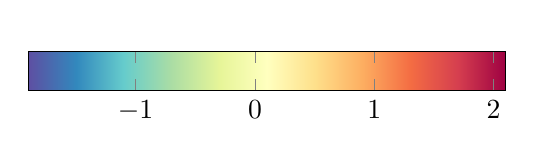
\begin{tikzpicture}
      \begin{axis}[
          hide axis,
          scale only axis,
          height=0pt,
          width=0pt,
          colormap name=Spectral_r,
          colorbar horizontal,
          point meta min=-1.9,
          point meta max=2.1,
          colorbar style={
              width=0.5\textwidth,
            }]
        \addplot [draw=none] coordinates {(0,0)};
      \end{axis}
    \end{tikzpicture}

  \end{subfigure}
  \caption{The error $\epsilon$ (\autoref{eq:action-log-error}) in the kinetic energy of the resting water column is plotted for different parameters of time step size $\lambda\in[0,1]$ and stiffness $k\in[500,1500]$ for $5\times 5$ datapoints. Each row shows one solver, where the left column are contour plots and the right column shows the same values in 3D for better visual clarity. The mapping from values to colours is shown in the bar at the bottom.}
  \label{fig:stability-k-lambda}
\end{figure}



The figure reveals a couple of interesting facts about the solvers in the chosen range of parameters. Firstly, it can be observed that in this scenario, the iterative solver vastly outperforms all other solvers in terms of stability and robustness, being stable across the entire range of tested parameters. There appears to be trough along the $k=1000$ line, while no discernable gradient in $\lambda$-direction can be observed. This means that all tested time step sized lead to roughly equally stable results, while one stiffness in particular results in slightly more stable simulations. This could be an indication that an optimized stiffness $k$, as is often derived for iterative solvers, is indeed important for optimal behaviour of the solver. Reducing the time step size on the other hand may not be as effective at improving accuracy in a scenario where relatively large time steps are tolerated, further motivating the use of a time step size closer to the largest stable value.

The \texttt{EOSSPH} and \texttt{SplitSPH} solvers behave as one might expect, with less stable behaviour as the stiffness $k$ and the time step size $\lambda$ are increased. This leads to the aforementioned conclusion that in order to achieve a desired level of both incompressibility and stability, $k$ should be increased until the incompressibility requirement is met and $\lambda$ decreased until the simulation is stable. \autoref{fig:stability-k-lambda} also shows that operator splitting helps improve stability and robustness by shifting the stable region of parameters in the positive $\lambda$-direction: whereas the \texttt{EOSSPH} solver has a steep gradient along the $k$-direction, with impractically low stiffnesses being drastically more stable, a more distinct second gradient along the $\lambda$-direction can be observed for the \texttt{SplitSPH} solver. This means that even for large values of $k$ a relatively small decrease in time step size can help significantly improve the stability of the simulation. For the \texttt{EOSSPH} solver one would expect the same to be true, but for much smaller time step sizes, which in turn increase the computational cost of the simulation.

\horizontalspacer

The same analysis can be made for varying viscosity $\nu$ and stiffness $k$. Once again, the iterative solver produces uninteresting data since it is stable across the entire range of parameters. The results for the two remaining solvers are shown in \autoref{fig:stability-k-nu}.


\begin{figure}[h]
  \centering
  \begin{subfigure}[t]{\textwidth}
    \centering
    \begin{tikzpicture}
      \begin{groupplot}[
          group style={
              group size=2 by 1,
              vertical sep=2cm,
              horizontal sep=2cm,
            },
          colormap name=Spectral_r,
          % colormap/viridis, 
          point meta min=-1.9,
          point meta max=2.1,
          view={0}{90},
          xlabel={$k$},
          ylabel={$\nu$},
          zlabel={$\epsilon$},
          width=0.45\textwidth,
          height=0.45\textwidth,
        ]
        \nextgroupplot[
          title={\texttt{EOSSPH}}
        ]

        \addplot3 [
          contour filled,
        ] table {500.0 0.0001 -1.775406581727304
            500.0 0.000575 -2.32132244869146
            500.0 0.00105 -2.72838334712473
            500.0 0.001525 -2.2153678376274346
            500.0 0.002 -2.353160080473529

            750.0 0.0001 -1.0878262651867756
            750.0 0.000575 -2.47644702914891
            750.0 0.00105 -2.815872847958961
            750.0 0.001525 -2.1609065301458084
            750.0 0.002 -2.187307968996441

            1000.0 0.0001 0.264343272412918
            1000.0 0.000575 -2.3625359371724493
            1000.0 0.00105 -2.216981147177807
            1000.0 0.001525 -2.2962975386348528
            1000.0 0.002 -2.469890546086413

            1250.0 0.0001 0.3461347056438925
            1250.0 0.000575 -0.08891009169294693
            1250.0 0.00105 -2.7797606338486998
            1250.0 0.001525 -2.527561905744824
            1250.0 0.002 -2.426099096775281

            1500.0 0.0001 0.3989528205702097
            1500.0 0.000575 0.1323516710959186
            1500.0 0.00105 0.013973700343225141
            1500.0 0.001525 -0.013803633754411246
            1500.0 0.002 -0.08659161795614237

          };

        \addplot3 [
          contour gnuplot={
              contour dir=z,
              levels={-2,-1.5,-1,-0.5,0,0.5,1,1.5,2},
              labels over line,
              draw color = black,
            },
          thick,
        ] table {500.0 0.0001 -1.775406581727304
            500.0 0.000575 -2.32132244869146
            500.0 0.00105 -2.72838334712473
            500.0 0.001525 -2.2153678376274346
            500.0 0.002 -2.353160080473529

            750.0 0.0001 -1.0878262651867756
            750.0 0.000575 -2.47644702914891
            750.0 0.00105 -2.815872847958961
            750.0 0.001525 -2.1609065301458084
            750.0 0.002 -2.187307968996441

            1000.0 0.0001 0.264343272412918
            1000.0 0.000575 -2.3625359371724493
            1000.0 0.00105 -2.216981147177807
            1000.0 0.001525 -2.2962975386348528
            1000.0 0.002 -2.469890546086413

            1250.0 0.0001 0.3461347056438925
            1250.0 0.000575 -0.08891009169294693
            1250.0 0.00105 -2.7797606338486998
            1250.0 0.001525 -2.527561905744824
            1250.0 0.002 -2.426099096775281

            1500.0 0.0001 0.3989528205702097
            1500.0 0.000575 0.1323516710959186
            1500.0 0.00105 0.013973700343225141
            1500.0 0.001525 -0.013803633754411246
            1500.0 0.002 -0.08659161795614237

          };

        % -----------------------------------------------------------------------------------------------

        \nextgroupplot[
          title={\texttt{SplitSPH}}
        ]
        \addplot3 [
          contour filled,
        ] table {500.0 0.0001 -1.8767772764572803
            500.0 0.000575 -2.3416484055223985
            500.0 0.00105 -2.5639797994737044
            500.0 0.001525 -2.1294955716798696
            500.0 0.002 -2.4178874158520314

            750.0 0.0001 -0.3789489823565821
            750.0 0.000575 -0.38952183595799644
            750.0 0.00105 -0.43842090302420045
            750.0 0.001525 -0.6347736181966993
            750.0 0.002 -0.7508543560061871

            1000.0 0.0001 -0.031326103139639266
            1000.0 0.000575 -0.07242829559226019
            1000.0 0.00105 -0.11023873875331318
            1000.0 0.001525 -0.12104401573951722
            1000.0 0.002 -0.14704307953599297

            1250.0 0.0001 0.08853083786483268
            1250.0 0.000575 0.0598088358013705
            1250.0 0.00105 0.032324896958478365
            1250.0 0.001525 -0.0011433828547922202
            1250.0 0.002 -0.011763766196926767

            1500.0 0.0001 0.16427613556411932
            1500.0 0.000575 0.12395010079299895
            1500.0 0.00105 0.10754724916022108
            1500.0 0.001525 0.07121548036732889
            1500.0 0.002 0.05102281432300632

          };
        \addplot3 [
          contour gnuplot={
              contour dir=z,
              levels={-2,-1.5,-1,-0.5,0,0.5,1,1.5,2},
              labels over line,
              draw color = black,
            },
          thick,
        ] table {500.0 0.0001 -1.8767772764572803
            500.0 0.000575 -2.3416484055223985
            500.0 0.00105 -2.5639797994737044
            500.0 0.001525 -2.1294955716798696
            500.0 0.002 -2.4178874158520314

            750.0 0.0001 -0.3789489823565821
            750.0 0.000575 -0.38952183595799644
            750.0 0.00105 -0.43842090302420045
            750.0 0.001525 -0.6347736181966993
            750.0 0.002 -0.7508543560061871

            1000.0 0.0001 -0.031326103139639266
            1000.0 0.000575 -0.07242829559226019
            1000.0 0.00105 -0.11023873875331318
            1000.0 0.001525 -0.12104401573951722
            1000.0 0.002 -0.14704307953599297

            1250.0 0.0001 0.08853083786483268
            1250.0 0.000575 0.0598088358013705
            1250.0 0.00105 0.032324896958478365
            1250.0 0.001525 -0.0011433828547922202
            1250.0 0.002 -0.011763766196926767

            1500.0 0.0001 0.16427613556411932
            1500.0 0.000575 0.12395010079299895
            1500.0 0.00105 0.10754724916022108
            1500.0 0.001525 0.07121548036732889
            1500.0 0.002 0.05102281432300632

          };
      \end{groupplot}
    \end{tikzpicture}

  \end{subfigure}
  \caption*{\begin{tiny}$\lambda=0.1, \nu_2=10^{-3}, h=0.02, N=1572, \rho_0 = 1, \gamma_1=1, \gamma_2=0.5$, Hexagonal sampling with $\sigma=0.015h$\end{tiny}}
  \caption{The error $\epsilon$ (\autoref{eq:action-log-error}) is plotted for different parameters of time step size $\lambda\in[0,1]$ and viscosity $\nu\in[10^{-4}, 2\cdot10^{-3}]$ for $5\times 5$ datapoints. The mapping from values to colours is the same as in \autoref{fig:stability-k-lambda}.}
  \label{fig:stability-k-nu}
\end{figure}


This graph reveals that for the \texttt{EOSSPH} solver, an increase in viscosity can improve stability, at least up to a certain value of $\nu$, while very inviscid fluids are more challenging to simulate stably. More interestingly this does not seem to apply as much to the solver with operator splitting, which shows an error gradient exclusively in the $k$-direction. This might be due to the fact that the viscosity in the tested parameter range is not large enough for inaccurate viscous forces to cause instability, which leaves only the pressure forces as a possible reason for instability. These pressure forces correct a predicted density when operator splitting is used, where increased viscosity affects the predicted density, but appears to have less influence on the instabilities resulting from inaccurately correcting these predicted densities - although there are too few data points to be conclusive. It might be interesting to further examine this behaviour by checking if the opposite is true for operator splitting that integrates pressure forces first and viscosity afterwards, to check if for such a solver stiffness becomes less relevant for stability if the viscosity is sufficiently high.

\chapter{Conclusion and Future Work}

In this report, the Navier-Stokes equations have been derived, discretized, initial conditions and boundary conditions discussed and three variations of a solver for the system of partial differential equations have been presented, each building up from a simple solver using an equation of state, through the concept of operator splitting towards an iterative solver with superior stability and incompressibility guarantees. Parameters that affect the stability, numerical viscosity and the quality of the initial sampling of the continuous fields into discrete particles have been analysed.

The generality of the SPH scheme as a method of discretizing and interpolating fields was highlighted, decoupling it from preconceptions about the more specific implementations that commonly use SPH to simulate fluids, such as the density invariant source terms and even Lagrangian frameworks not being related to SPH by necessity but rather through choice. Gaussian-like kernels in particular, which are often taken for granted in SPH literature, were appreciated and possible reasons for their widespread use were given. An uncommon form of an iterative solver that more directly shows the connection between equation-of-state based solvers and more elaborate iterative solvers commonly in use was given, proving that the hurdle towards implementing a solver that can uphold incompressibility might not be as high as it seems.

A particular emphasis was placed on discussing how a field can be discretized to yield initial conditions that prevent aliasing artefacts and how the lattice that a field is sampled with, whether particles of uniform masses or densities are sampled and if a regular or pseudorandomly jittered configuration is chosen can influence the simulation quality in conjunction. This is a section of the report in that could use a more thorough investigation into what causes numerical viscosity and what parameters could positively affect this behaviour.

The frequency of oscillations observed when using the absolute density to enforce the continuity equation was analysed and some relatively speculative claims where made that also warrant further investigation, such as the exact nature of the relation between stiffness, speed of sound, oscillation frequency and the number of iterations of a solver. This might be an area of particular interest, since unwelcome oscillations can be seen as a major flaw in many SPH-based fluid solvers.

All in all, there are many angles from which the observations laid out in this report could be more thoroughly theoretically underpinned and empirically validated or taken as motivation to investigate a perhaps less vigorously researched branch of improvements to fluid simulation with Smoothed particle hydrodynamics, and the possibilities for future work in this field seem endless.




\printbibliography[
  heading=bibintoc,
  title={Bibliography}
]
\end{document}